%%\PassOptionsToPackage{table}{xcolor}
\documentclass[10pt]{article}
%
%%%%%%%%%%%%%%%%%%%%%%%%%%%%%%%%%%%%
%% Common preamble
%%%%%%%%%%%%%%%%%%%%%%%%%%%%%%%%%%%%
% PAGE
\usepackage{fullpage} % uncomment this when changing to jour/conf style
\usepackage{verbatim} 
% FONTS
%%\usepackage{lmodern} % enhanced version of computer modern
%%\usepackage[T1]{fontenc} % for hyphenated characters and textsc in section title
%%\usepackage{microtype} % some compression
\usepackage{times}
\usepackage{setspace} % For double line spacing
\doublespacing
% MATH
\usepackage{amssymb}
\usepackage{mathtools} % contains amsmath which comes with align
\usepackage{amsthm} % newtheorem stuff
\usepackage{bm} % for bold math (use $\boldsymbol{}$)
% COLOR
\usepackage[table,usenames,dvipsnames]{xcolor}
%%
% REFERENCING
\usepackage[square,sort&compress,numbers]{natbib} %sorts bibs when they are collectively cited
\usepackage[colorlinks=true,pdfborder={0 0
0},citecolor=RoyalBlue,linkcolor=black,urlcolor=Magenta]{hyperref}
\usepackage{cleveref} %%% IMPORTANT: cleveref comes before \newtheorem commands
   \crefname{figure}{Figure}{Figures}
   \crefname{table}{Table}{Tables}
   \crefname{theorem}{Theorem}{Theorems}
   \crefname{lemma}{Lemma}{Lemmas}
   \crefname{claim}{Claim}{Claims}
   \crefname{section}{Section}{Sections}
   \crefname{observation}{Observation}{Observations}
   \crefname{note}{Note}{Notes}
%%
% TABLES
\usepackage{multirow}
\usepackage{booktabs} % provides toprule, bottomrule, midrule
\usepackage{array} % new implementation of tabular & array with lots of enhancements

%%
% FIGURES
\usepackage{graphicx}
\graphicspath{./figs}
\usepackage{grffile} % to set right names of files
%%
% CAPTIONS
\usepackage{caption}
\usepackage{subcaption} % supersedes subfigure & subfloat. try using options
%%
% LISTS
\usepackage{enumitem} %\begin{itemize}[leftmargin=*]
%% inline
\newlist{inline}{enumerate*}{1}
\setlist[inline]{before=\unskip{: }, itemjoin={{; }}, itemjoin*={{; and }}, label={(\roman*)}}
% ALGO
\usepackage[ruled,linesnumbered]{algorithm2e}
%% comments & todo
\renewcommand*{\thesection}{S\arabic{section}}
\renewcommand*{\thesubsection}{S\arabic{section}.\arabic{subsection}}
\renewcommand*{\thefigure}{S\arabic{figure}}    
\renewcommand*{\thetable}{S\arabic{table}}    
\newcommand{\asd}{\alpha_s}
\newcommand{\afm}{\alpha_{\ell}}
\newcommand{\ald}{\alpha_{\ell d}}
\newcommand{\mooreRange}{r_\mathrm{M}}
\newcommand{\consume}{\mathrm{Pop}}
\newcommand{\locality}{\mathrm{L}}
\newcommand{\export}{\mathrm{Export}}
\newcommand{\import}{\mathrm{Import}}
\newcommand{\process}{\mathrm{Proc}}
\newcommand{\produce}{\mathrm{Prod}}
\newcommand{\veg}{\mathrm{V}}
\newcommand{\temp}{\mathrm{T}}
\newcommand{\similarity}{\mathcal{S}}
\newcommand{\kmax}{k_{\max}}
\newcommand{\infest}{\rho}
\usepackage{xr}
\externaldocument[M:]{mcnitt_tuta}


\newcommand{\aacomment}[1]{({\color{magenta}AA: #1})}
\newcommand{\jmcomment}[1]{({\color{blue}JM: #1})}
\usepackage[colorinlistoftodos]{todonotes}
\newcommand{\TODO}[1]{\todo[inline,color=red!10,size=\small]{#1}}
%% COMMANDS
\newcommand{\comp}[1]{\overline{#1}}  %{\widetilde{#1}}
\DeclareMathOperator{\Var}{Var}
\DeclareMathOperator{\Cov}{Cov}
\DeclareMathOperator{\bigo}{O}
\DeclareMathOperator{\bigom}{\Omega}
\DeclareMathOperator{\davg}{d_{avg}}
\DeclareMathOperator*{\argmax}{arg\,max}
\DeclareMathOperator*{\argmim}{arg\,min}
% Note: \deg is already defined. If not
% \newcommand{\deg}{\mathrm{o}}
\newcommand{\expect}{\mathbb{E}}
%
\newcommand{\ceil}[1]{\left\lceil #1 \right\rceil}
\newcommand{\floor}[1]{\left\lfloor #1 \right\rfloor}
%
\newcommand{\reals}{\mathbb{R}}
\newcommand{\field}{\mathbb{F}}
\newcommand{\integers}{\mathbb{Z}}
%
\newtheorem{theorem}{Theorem}[]{\bfseries}{\itshape} 
\newtheorem{lemma}[theorem]{Lemma}{\bfseries}{\itshape}
\newtheorem{claim}[theorem]{Claim}{\bfseries}{\itshape}
\theoremstyle{definition}
\newtheorem{definition}[theorem]{Definition} % {\bfseries}{\itshape}
\newtheorem{observation}[theorem]{Observation} % {\bfseries}
\newtheorem{condition}[theorem]{Condition} % {\bfseries}{\itshape}
\newtheorem{note}[theorem]{Note} % {\bfseries}{\itshape}
% ROMAN NUMERALS
\makeatletter
\newcommand{\rmnum}[1]{\romannumeral #1}
\newcommand{\Rmnum}[1]{\expandafter\@slowromancap\romannumeral #1@}
\newcommand{\tuta}{\emph{T.~absoluta}}
\makeatother
% TWO VERSIONS
%% \usepackage{etoolbox}
%% \newtoggle{withappendix}
%% \toggletrue{withappendix} % comment this if you want journal version
%% Usage: iftoggle{withappendix}{}{}
%%
%% math operator
%% \DeclareMathOperator{\sgn}{sgn}
% CODEBOX
%% \usepackage[framemethod=tikz]{mdframed}
%% \newmdenv[linecolor=black!10,innerlinewidth=0pt, roundcorner=4pt,innerleftmargin=6pt,
%% font=\ttfamily,innerrightmargin=6pt,innertopmargin=6pt,
%% innerbottommargin=6pt,backgroundcolor=black!10]{codeblock}
%%%%%%%%%%%%%%%%%%%%%%%%%%%%%%%%%%%%
%% preamble ends
%% from now on, draft specific
%%%%%%%%%%%%%%%%%%%%%%%%%%%%%%%%%%%%
\usepackage{authblk}
%% \RequirePackage[l2tabu, orthodox]{nag}
\title{Supplementary material: Assessing the Multi-pathway Threat from an Invasive Agricultural
Pest: \emph{Tuta~absoluta} in Asia}
\author[1]{Joseph~McNitt}
\author[2]{Young~Yun~Chungbaek}
\author[2]{Henning~Mortveit}
\author[2]{Madhav~Marathe}
\author[3]{Mateus~Ribeiro~de~Campos}
\author[3]{Nicolas~Desneux}
\author[4,5,6]{Thierry~Br\'{e}vault}
\author[7]{Rangaswamy Muniappan}
\author[2]{Abhijin~Adiga}
\affil[1]{Epic Systems Corporation, United States}
\affil[2]{Biocomplexity Institute \& Initiative, University of Virginia}
\affil[3]{French National Institute for Agricultural Research}
\affil[4]{BIOPASS, CIRAD-IRD-ISRA-UCAD, Dakar, Senegal}
\affil[5]{CIRAD, UPR AIDA, F-34398 Montpellier, France}
\affil[6]{Universit\'{e} de Montpellier, CIRAD, Montpellier, France}
\affil[7]{Feed the Future Integrated Pest Management Innovation Lab,
Virginia Tech}
\date{}

\begin{document}
\maketitle

\section{Data}
\label{sec:data}
Table~\ref{tab:data} lists all publicly available datasets incorporated in
our model and analysis. Table~\ref{tab:countryData} provides country-specific data sources,
literature and reports used in the model and for validation. They are further tagged
based on the information they provide for different aspects of the model.
Table~\ref{tab:bgdData} provides incidence reports from Bangladesh.

%%
\rowcolors{2}{white}{gray!15} % For this to work, put \PassOptionsToPackage{table}{xcolor} before \documentclass
\newcommand{\mrow}[1]{\multirow{2}{*}{\parbox{1cm}{#1}}}
\begin{table}[ht]
    \caption{Global data sets used for model construction. \label{tab:data}}
    \centering
\begin{tabular}{ccc}
    \hline
 {Data} & {Source} &  {Spatial or temporal resolution} \\\hline
Temperature &
WorldClim~\cite{hijmans2005very} &
2.5 arc min., monthly.  \\
%%
Precipitation &
GPCC~\cite{precip} & 2.5 arc deg., monthly.\\

Humidity &NASA \cite{humidity}&1 arc deg., monthly. \\

%%
NDVI &NEO \cite{ndvi}& 0.1 arc deg., monthly. \\
%%
Country Production & FAO \cite{faostatProduction} &country, yearly.\\
%%
Shape files of study region & ADC Worldmap \cite{ADCW2018} &
country/province/district.\\
%%
Cell Production &Mapspam \cite{spam}&5 arc min., yearly. Gives vegetable and potato data.\\
%%
Consumption&FAO \cite{faostatConsumption}&country, yearly. \\
%%
Population & Landscan\cite{pop} & 5 arc min. \\
%%
Cities & MAXMIND \cite{maxmind}& city resolution\\
%%
Distance between cities & Google API \cite{distance-matrix}&city
resolution\\\hline
\end{tabular}
\end{table}
%% 		& Tomato production & & & FAOSTAT  \\	
%% 		& Vegetable production distribution & & & SPAM  &5 min. $\times$ 5 min. & \\	
%% 		& Production seasonality & & & &Country level, Monthly &    \\
%%         \hline
%% 	    & Tomato consumption & & & FAO & 
%%         Country, Annual & 2011 \\	 
%% 		& Population & & & Landscan & 0.008333 $\times$ 0.008333 degrees &   \\
%%         & Per Capita Income & & & FAO\aacomment{check}
%% 		& Country & 2013 \\
%%         \hline
%% 	    & Tomato import/exports & & & FAOSTAT &Country, Annual& 2013 \\
%% 		& Cities and their population & & & MAXMIND &City/town & 2017  \\
%% 	    & City distances & & & Google Maps, Distance matrix API & City & 2017  \\
%%         \hline
%% 	    & \tuta{} incidence reports & \\
%% 		\hline
    %% \newline
    %% $^\dagger$The appropriate references are provided in the Supplementary
    %% Information.
\begin{table}[!h]
\caption{Country-specific data obtained from reports, peer-reviewed
articles and experts' inputs.
\label{tab:countryData}}
\centering
\rowcolors{3}{gray!15}{white} % For this to work, put \PassOptionsToPackage{table}{xcolor} before \documentclass
\begin{tabular}{*{8}{c}}
\toprule
\mrow{Country} & \mrow{Seasons} & \mrow{Production} & \mrow{Consumption} &
\multicolumn{2}{c}{Domestic trade} & \mrow{Processing}& \mrow{International trade} \\
 & & & & Markets & Flows & & \\
\midrule
Bangladesh & \cite{bbs2017} & \cite{bbs2017} & \cite{faostat} & \cite{bbs2017} & -- &
\cite{weinberger2005vegetable,bbs2017} & \cite{EIIndia2015}\\
Cambodia & \cite{sokhen2004vegetable,genova2006postharvest,buntong2013} &
\cite{sokhen2004vegetable,genova2006postharvest}
&\cite{sokhen2004vegetable}&\cite{sokhen2004vegetable}&\cite{sokhen2004vegetable}&
--&\cite{moustier2007,sokhen2004vegetable}\\
Indonesia & \cite{grubben1989,arsanti2015} & \cite{grubben1989,arsanti2015} &
\cite{faostat} & --&-- &-- & \cite{faostat}\\
Laos & \cite{kethonga2004} & \cite{kethonga2004} & \cite{kethonga2004} &
\cite{kethonga2004} & \cite{kethonga2004} & -- &
\cite{moustier2007,kethonga2004} \\
Malaysia &-- & \cite{malaysiaMOA,hengky2016} &\cite{faostat} &-- &-- & -- &
\cite{faostat} \\
Myanmar & -- & \cite{kraas2006megacity,SanSanYi2008} & \cite{Moe2013} &
&\cite{kraas2006megacity} \\
Philippines & \cite{psa2017,batt2011} &  \cite{psa2017} & \cite{concepcion2009} &
\cite{concepcion2011} &  & & {ignored~\cite{concepcion2011}} \\
Singapore & -- & \cite{faostat} & imp.-exp. & city & ignored \\
Thailand & \cite{itharattana1996} & \cite{mict2013,vanitAnunchai2006,itharattana1996}
&\cite{vanitAnunchai2006} &\cite{vanitAnunchai2006,itharattana1996} &
\cite{itharattana1996} & \cite{mict2013}\\
Vietnam & \cite{Vien2003,wijk2007,huong2013} & \cite[Table~16]{wijk2007}
(2003) &
\cite[Table~23]{wijk2007} & \cite{moustier2007,wijk2007,cadilhon2006} & \cite{moustier2007,wijk2007,cadilhon2006} &
\cite{wijk2007,jica2012vietnam} &
\cite{moustier2007,wijk2007} \\
\bottomrule
\end{tabular}
\end{table}
%%

\begin{table}[!h]
\caption{Data of \tuta{} infestation for Bangladesh (source: Bangladesh
Agricultural Research Institute) and neighbouring region of India. \label{tab:bgdData}}
\centering
\rowcolors{1}{white}{gray!15} % For this to work, put \PassOptionsToPackage{table}{xcolor} before \documentclass
\begin{tabular}{*{3}{c}}
\toprule
Location & Coordinates & Month of first detection of \tuta{} \\
\midrule
Chaklarhat, Panchagarh district & $26.19^\circ$ N, $88.43^\circ$ E & May 2016 \cite{hossain2016first} \\
Umiam~\cite{sankarganesh2017}, 
BARI Research Field, Gazipur district & $23.99^\circ$ N, $90.42^\circ$ E & January 2017 \\
RARS, Akbarput, Moulvibazar district & $24.25^\circ$ N, $91.45^\circ$ E & February 2017 \\
Lalakhal, Jointiapur, Sylhet district & $25.07^\circ$ N, $92.09^\circ$ E & February 2017 \\
Palashbari, Gaibandha district & $25.15 ^\circ$ N, $89.23 ^\circ$ E & March 2017 \\
Battara, Bogra district & $24.48^\circ$ N, $89.25^\circ$ E & February 2017 \\
Barura, Comilla district & $23.22^\circ$ N, $91.06^\circ$ E & March 2017 \\
Patengali, Jessore district & $23.09 ^\circ$ N, $89.10 ^\circ$ E & March
2017 \\ \hline
Umiam, Meghalaya India &  & January 2017 \cite{sankarganesh2017} \\
\bottomrule
\end{tabular}
\end{table}

%% \begin{figure}[ht]\label{baselineMyanmar}
%% \centering
%% \begin{subfigure}[b]{.47\textwidth}
%% \centering
%% 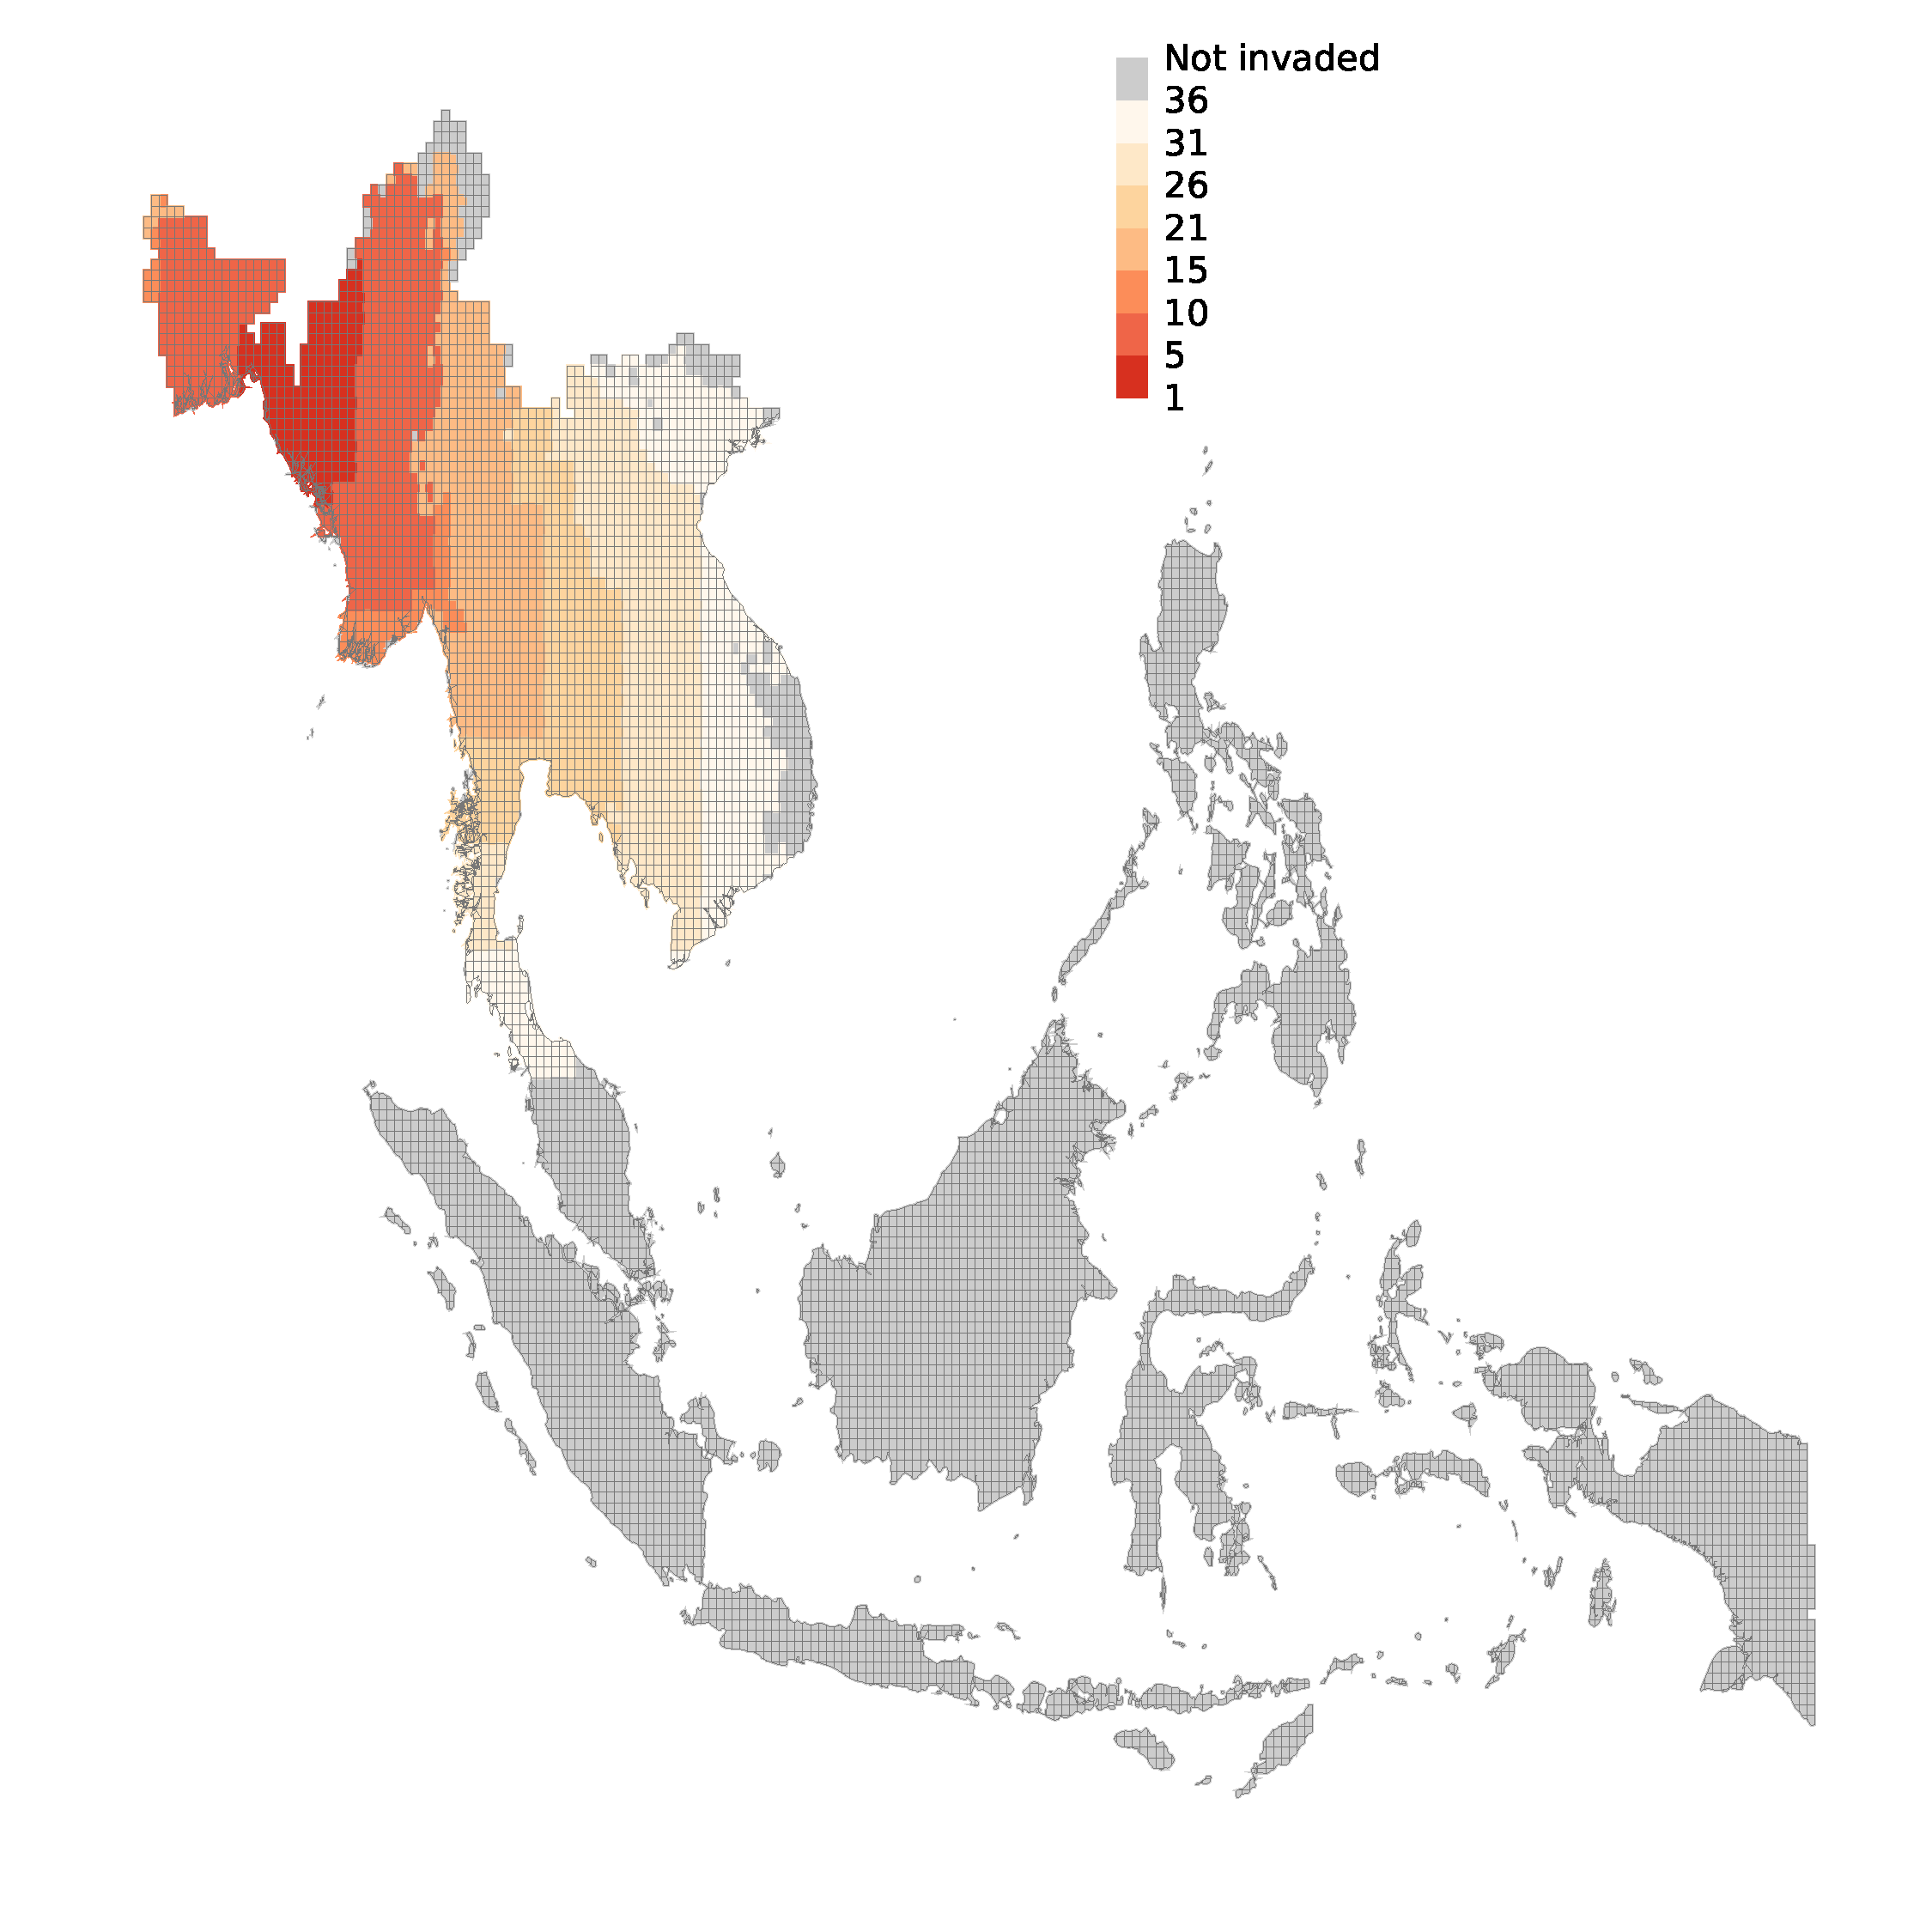
\includegraphics[width=\textwidth]{figs/plot_Myanmar2.pdf}
%% \caption{Moore neighborhood of 2, baseline model}
%% \end{subfigure}
%% \end{figure}
%

%% \begin{figure}[ht]
%%         \centering
%% \begin{subfigure}[b]{.45\textwidth}
%%         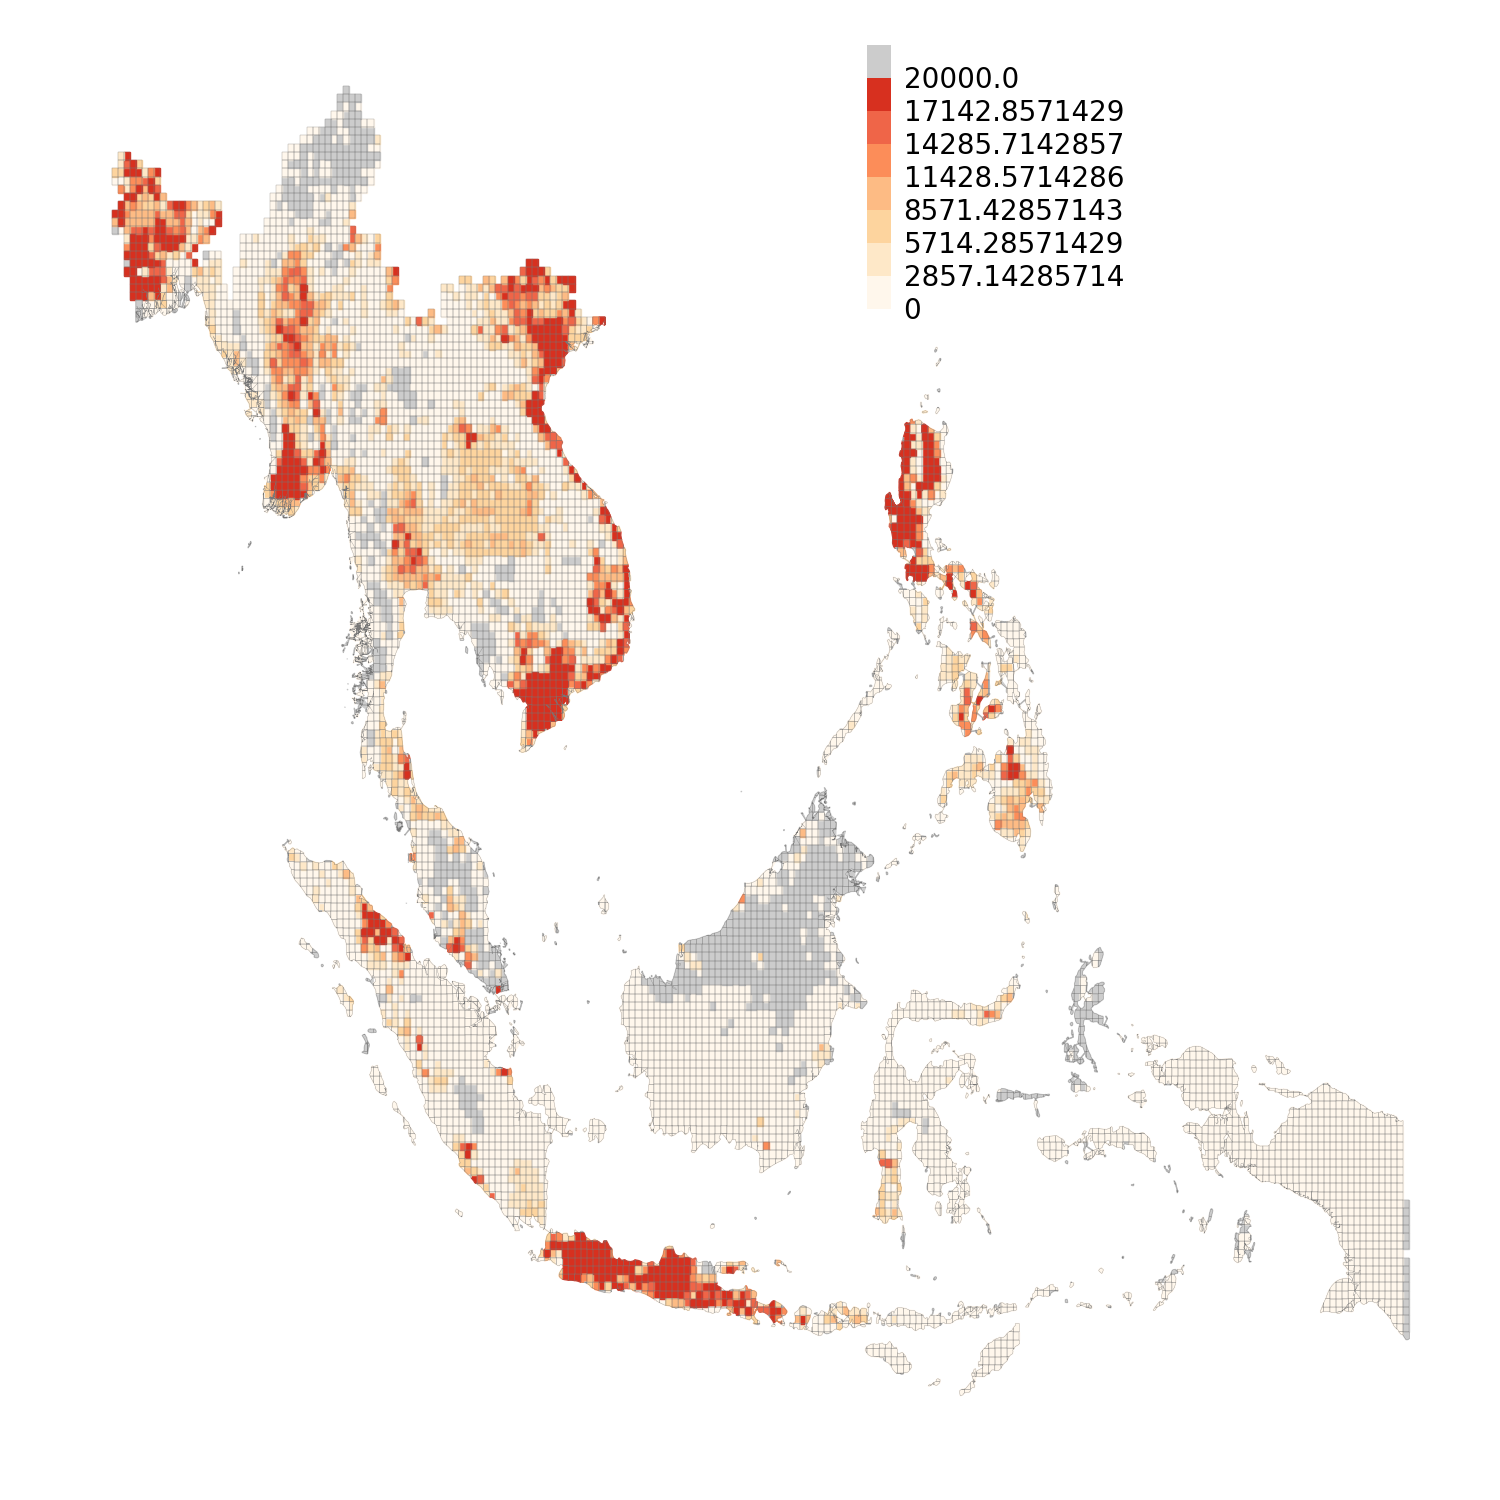
\includegraphics[width=\textwidth]{figs/mapspam_raw.png}
%%         \caption{ Mapspam Vegetable Production}
%% 
%% \end{subfigure}
%% %
%% \begin{subfigure}[b]{.45\textwidth}
%%         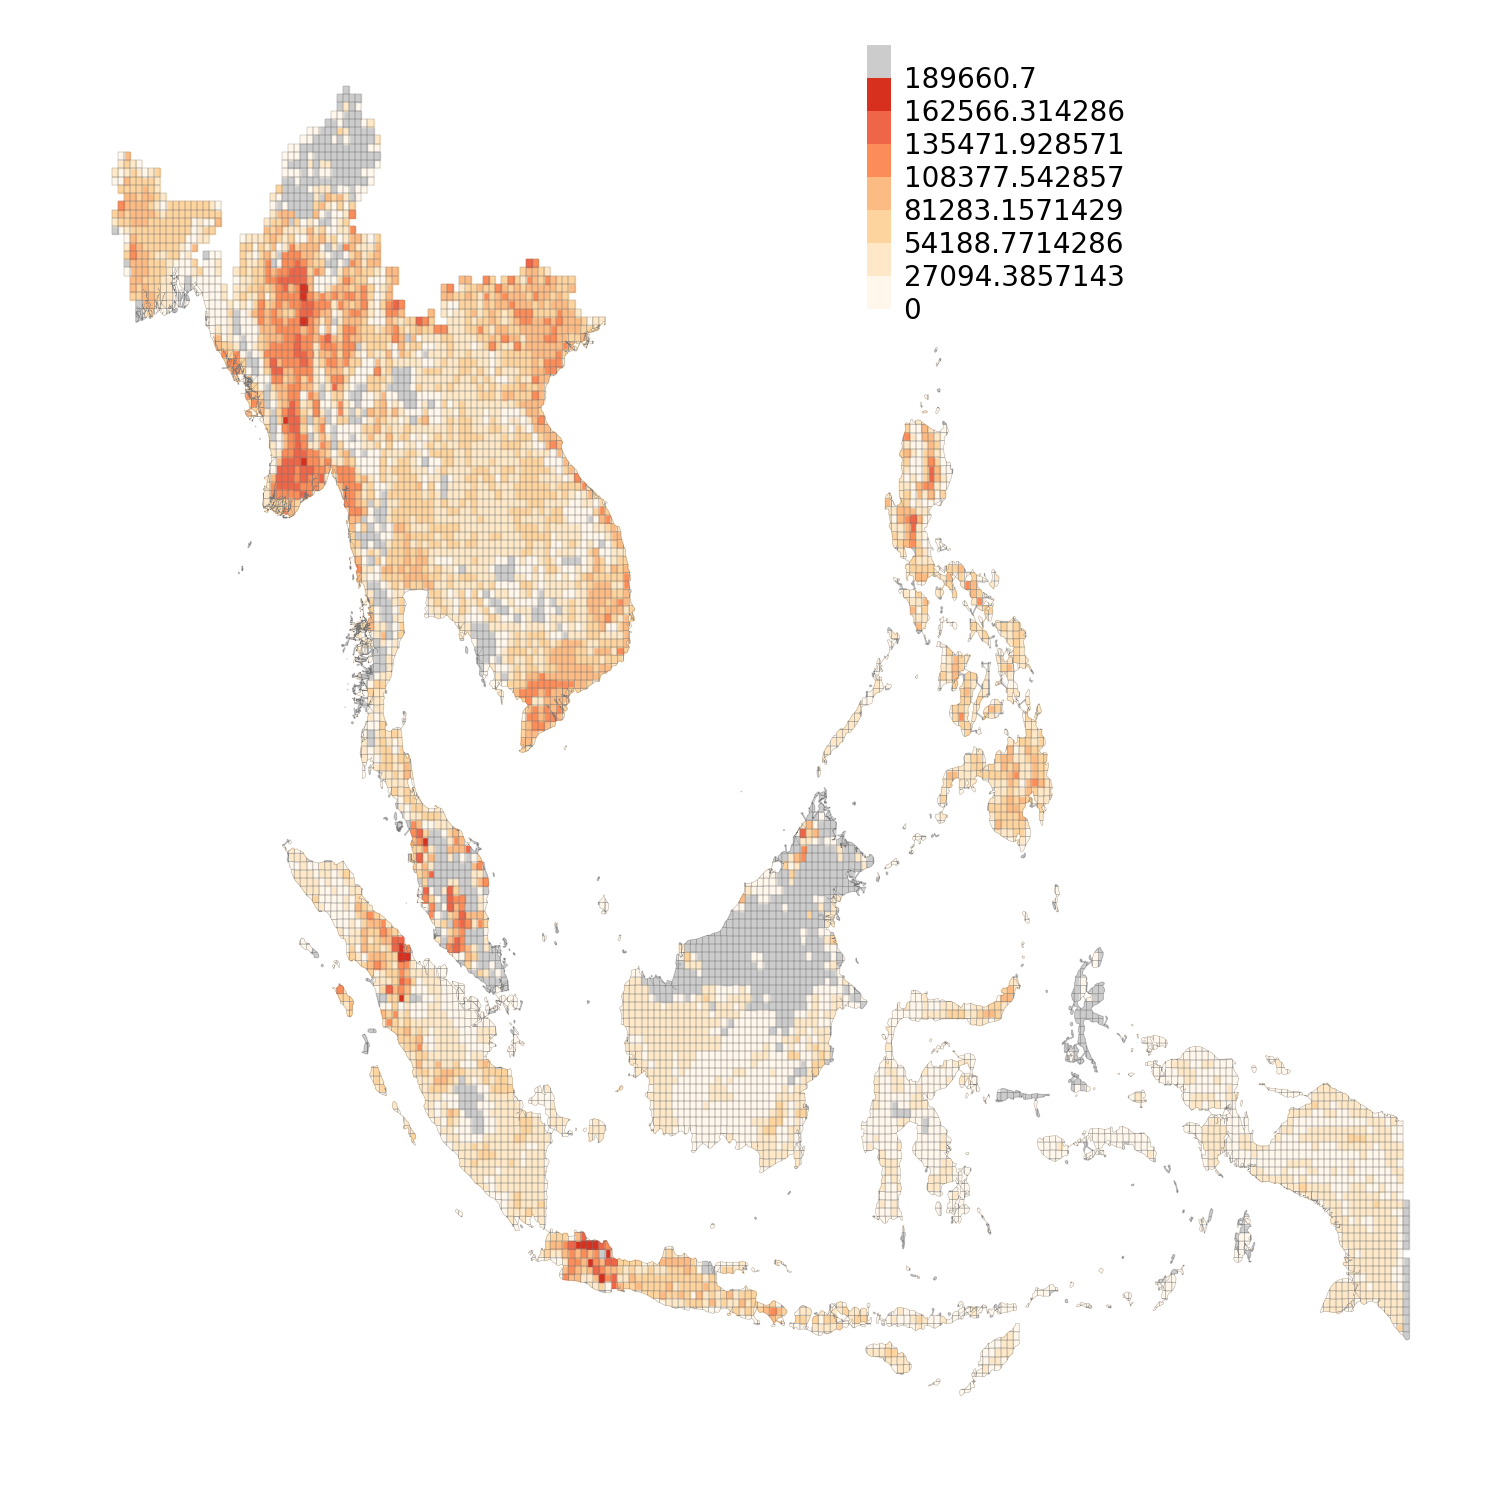
\includegraphics[width=\textwidth]{figs/mapspam_yield.png}
%%         \caption{Mapspam Vegetable Yield}
%% \end{subfigure}
%% \caption{}
%% \end{figure}
%
%% \begin{figure}[ht]
%% 
%% \begin{subfigure}[b]{.45\textwidth}
%%         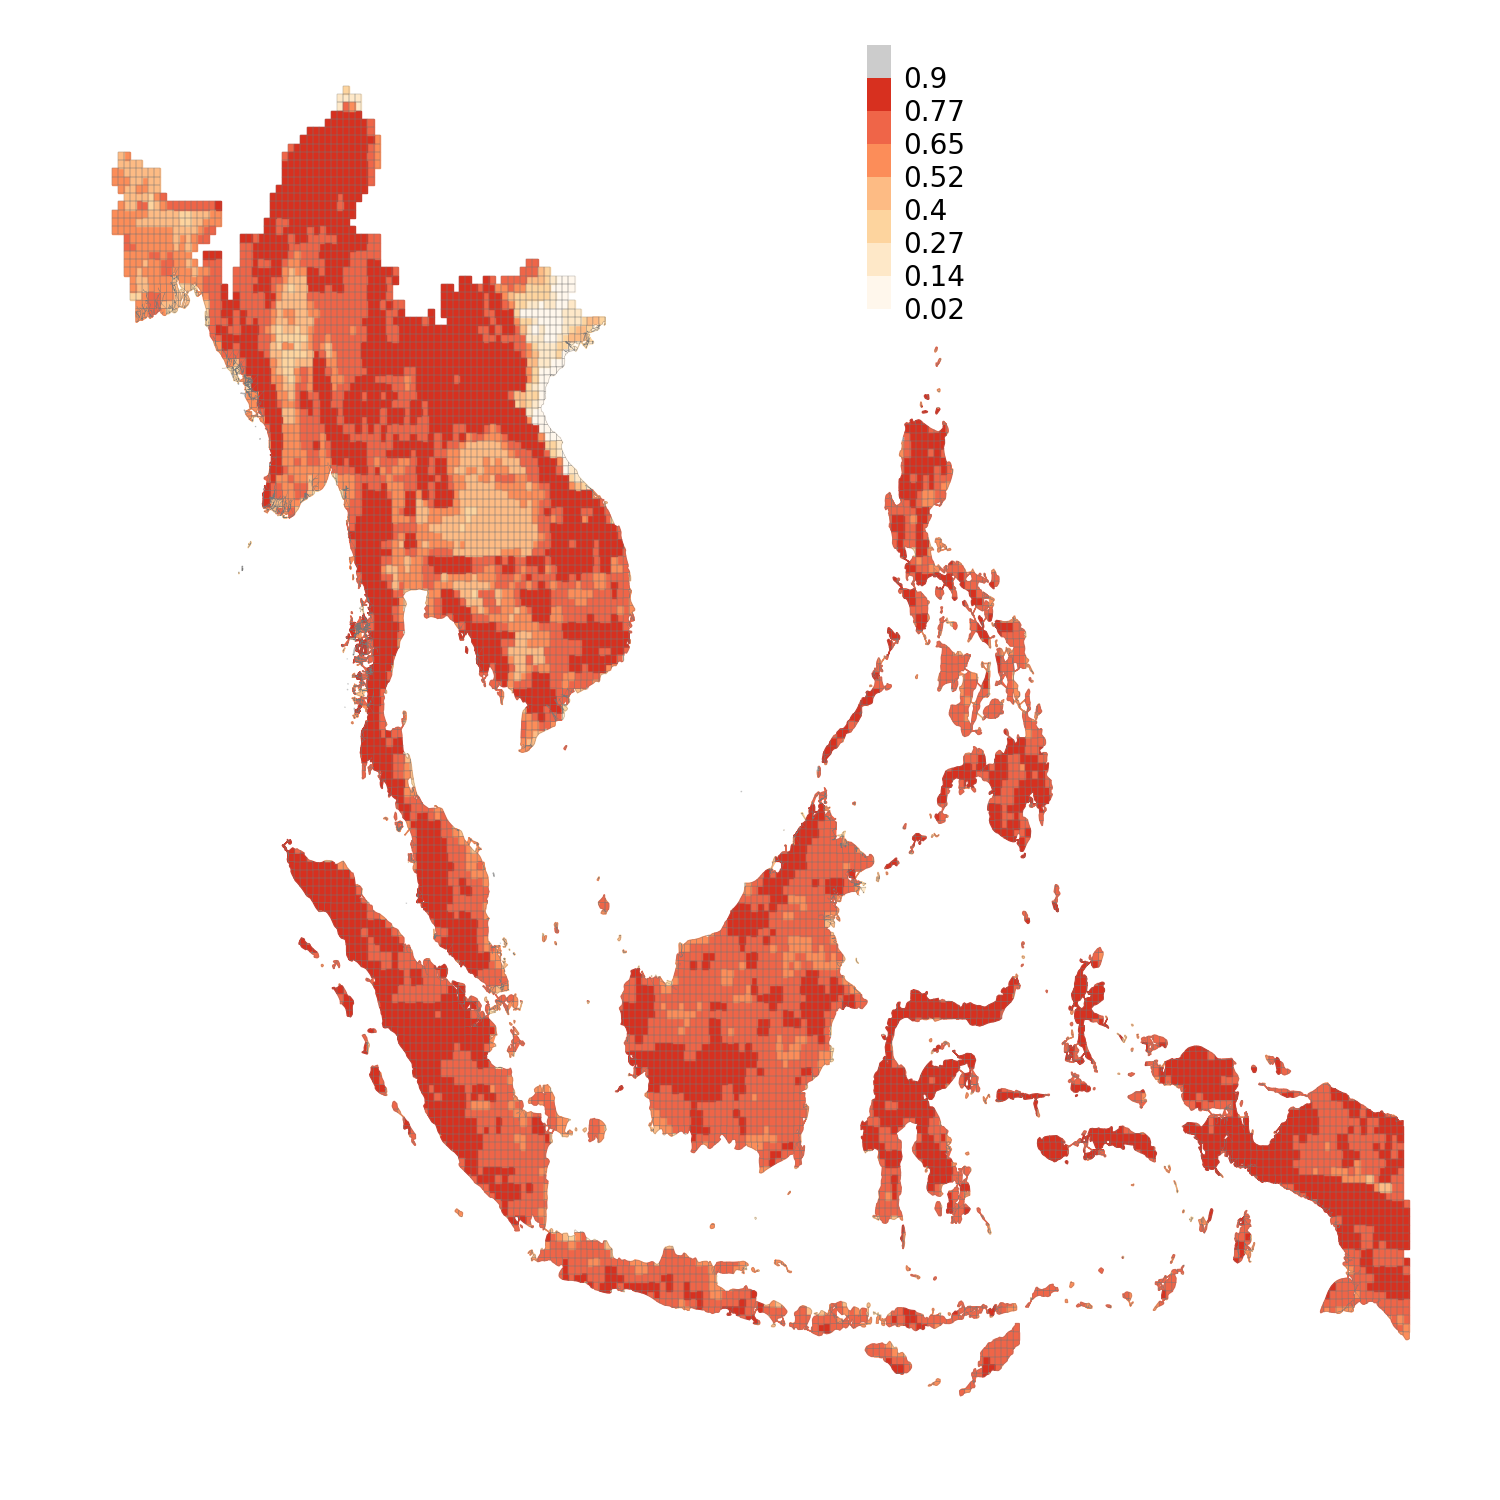
\includegraphics[width=\textwidth]{figs/heatmap_ndvi0.png}
%%         \caption{NDVI Jan.}
%% \end{subfigure}
%% %
%% \begin{subfigure}[b]{.45\textwidth}
%%         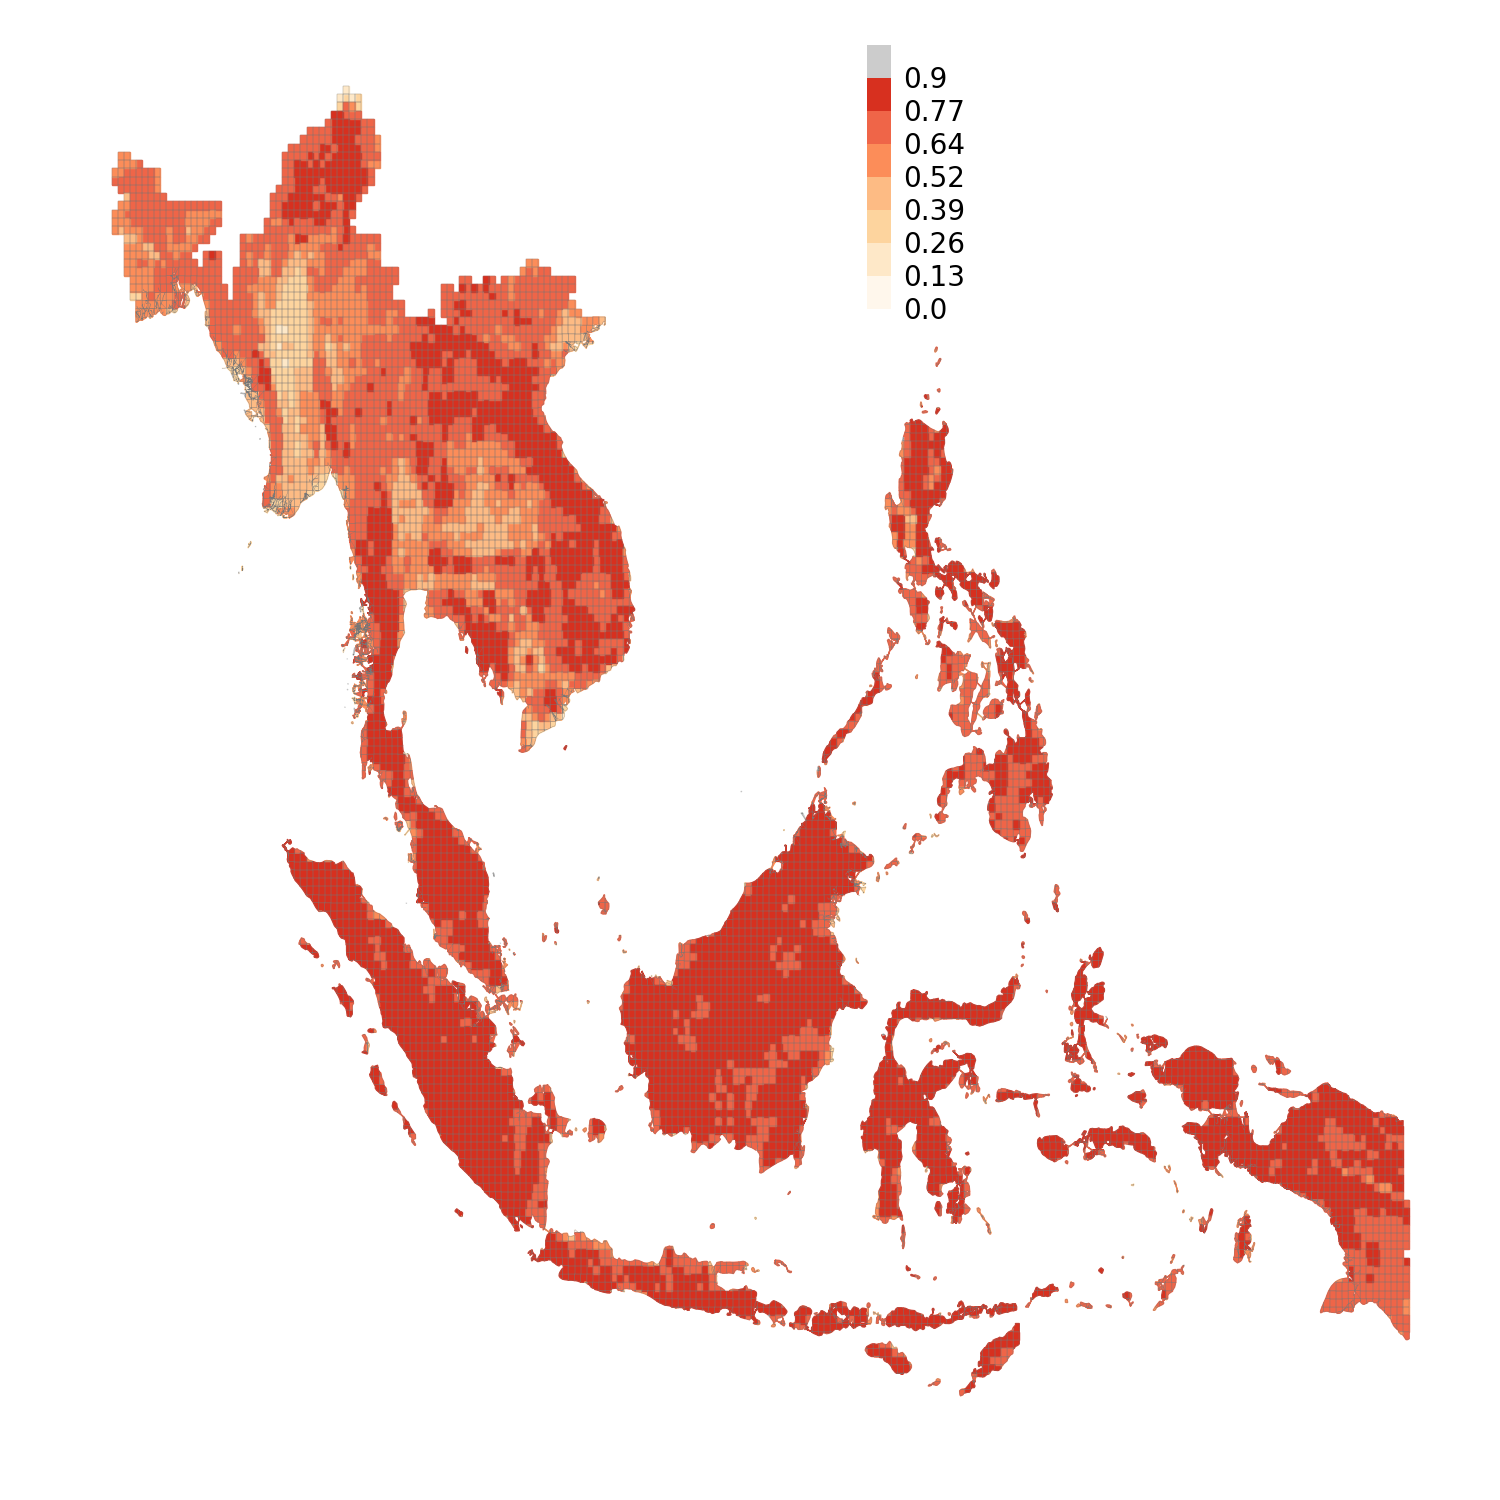
\includegraphics[width=\textwidth]{figs/heatmap_ndvi3.png}
%%         \caption{NDVI Apr.}
%% \end{subfigure}
%% %
%% \begin{subfigure}[b]{.45\textwidth}
%%         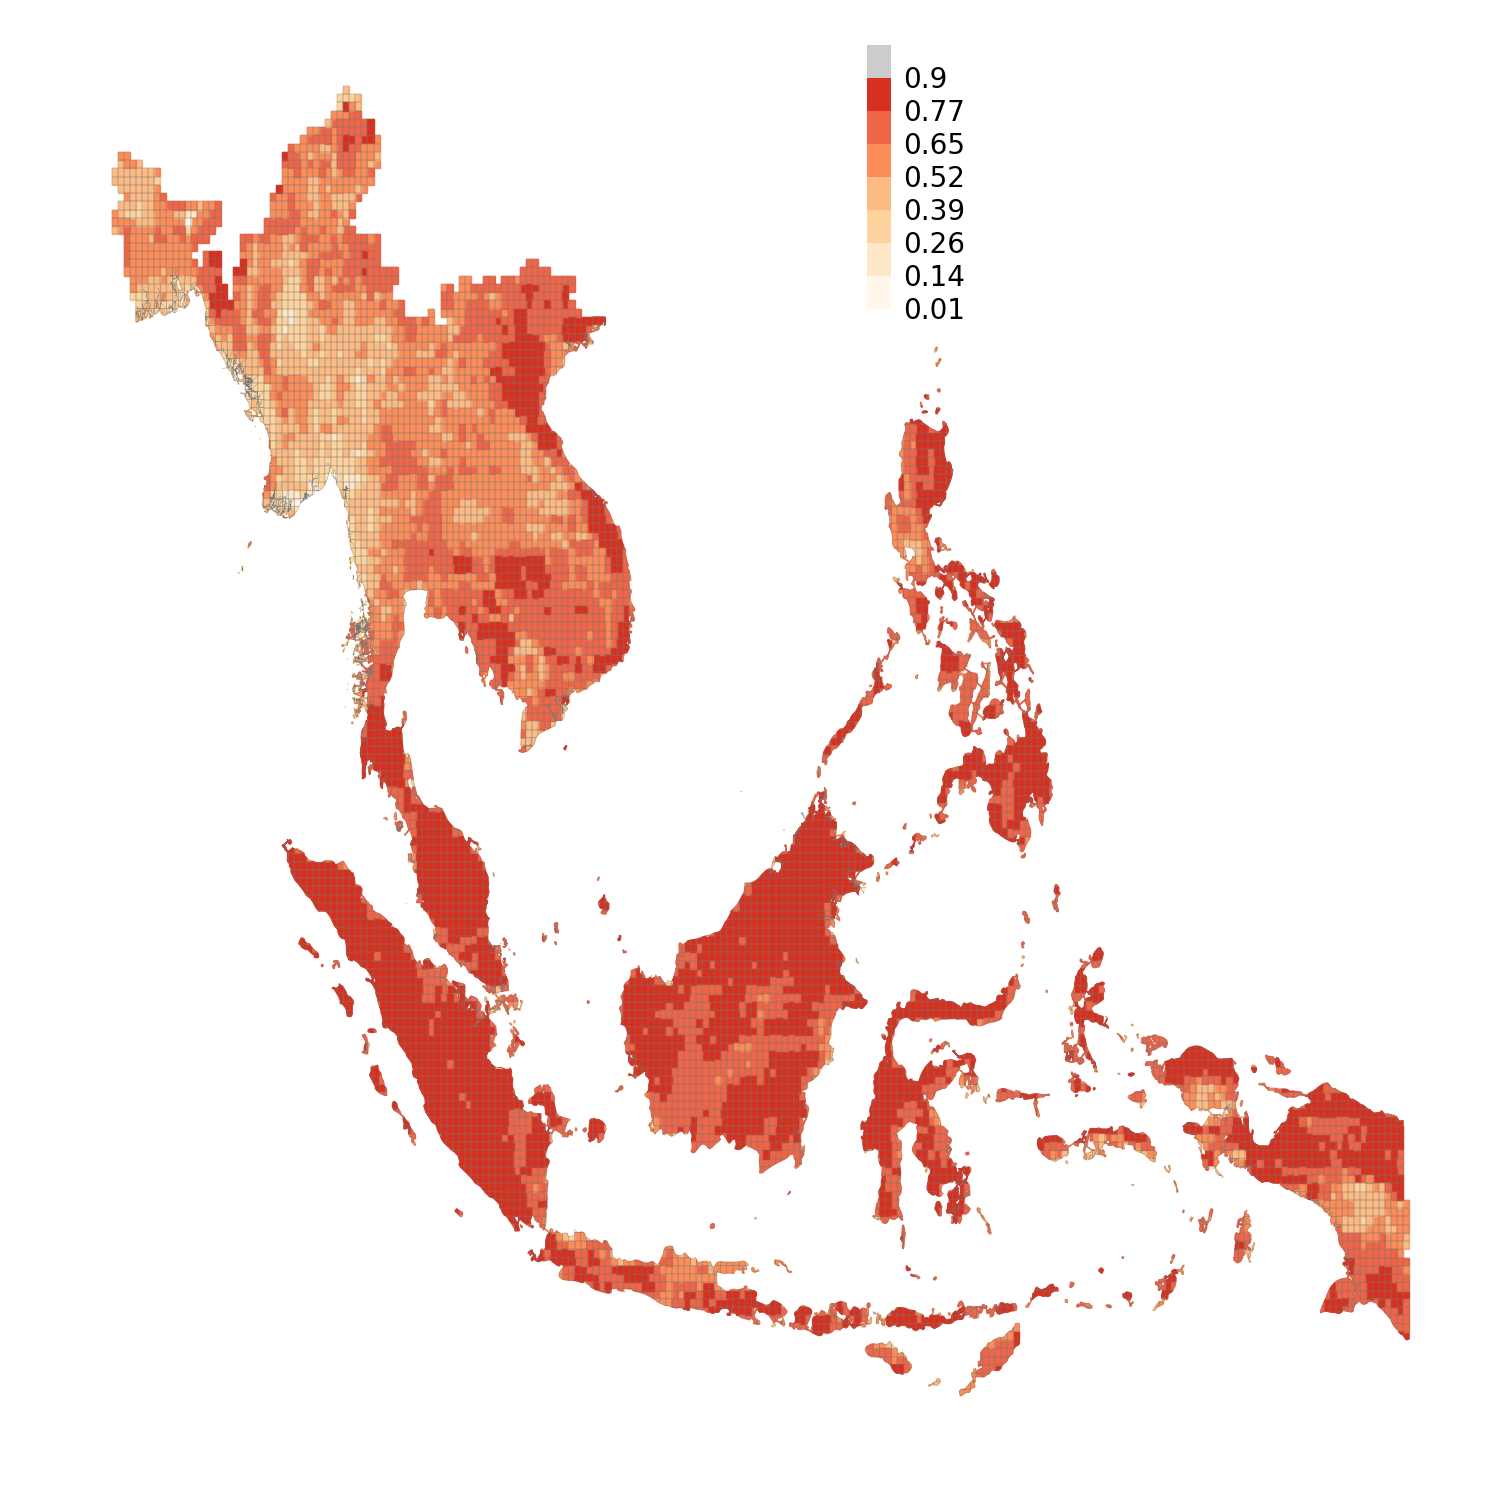
\includegraphics[width=\textwidth]{figs/heatmap_ndvi6.png}
%%         \caption{NDVI July}
%% \end{subfigure}
%% %
%% \begin{subfigure}[b]{.45\textwidth}
%%         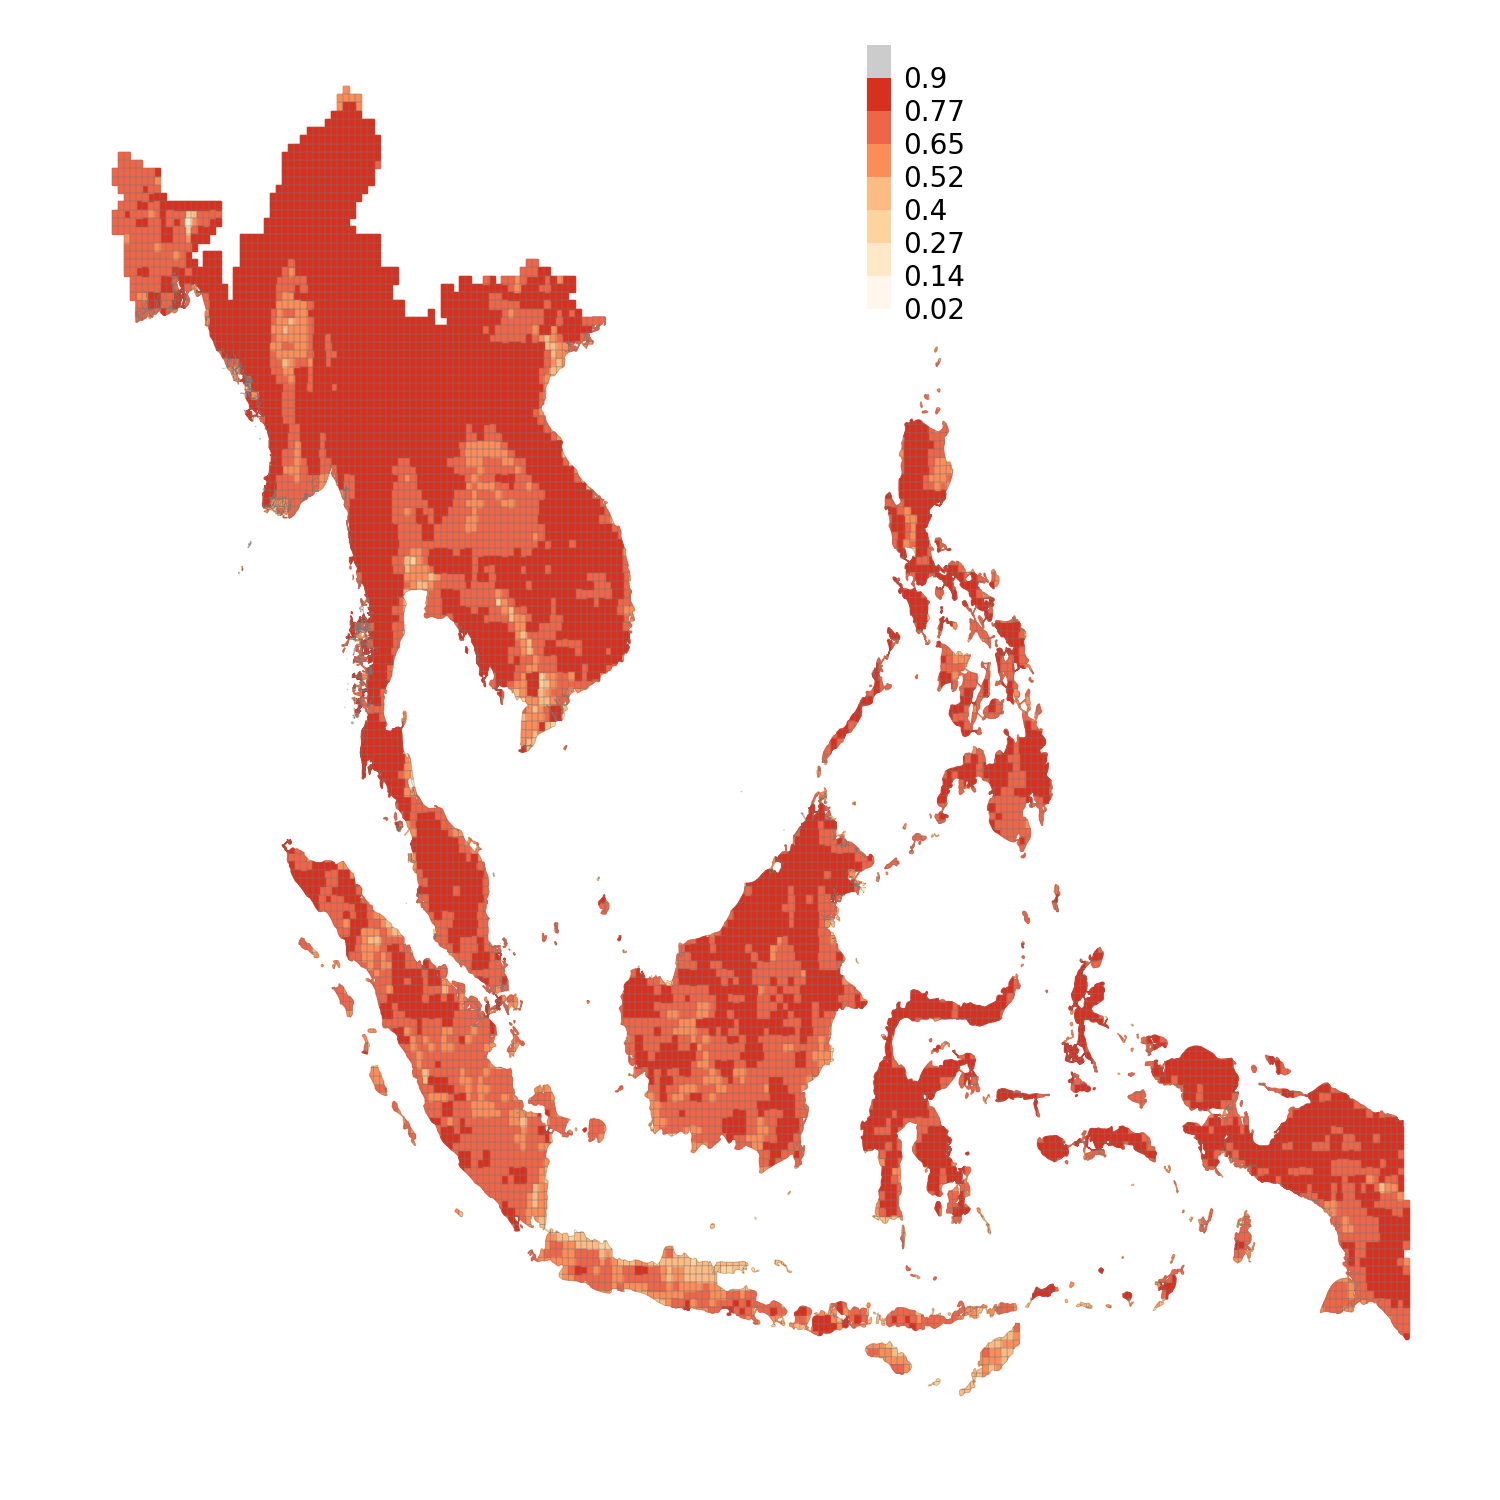
\includegraphics[width=\textwidth]{figs/heatmap_ndvi9.png}
%%         \caption{NDVI Oct.}
%% \end{subfigure}
%% 
%% \end{figure}
%
%% \begin{figure}[ht]
%% \begin{subfigure}[b]{.45\textwidth}
%%         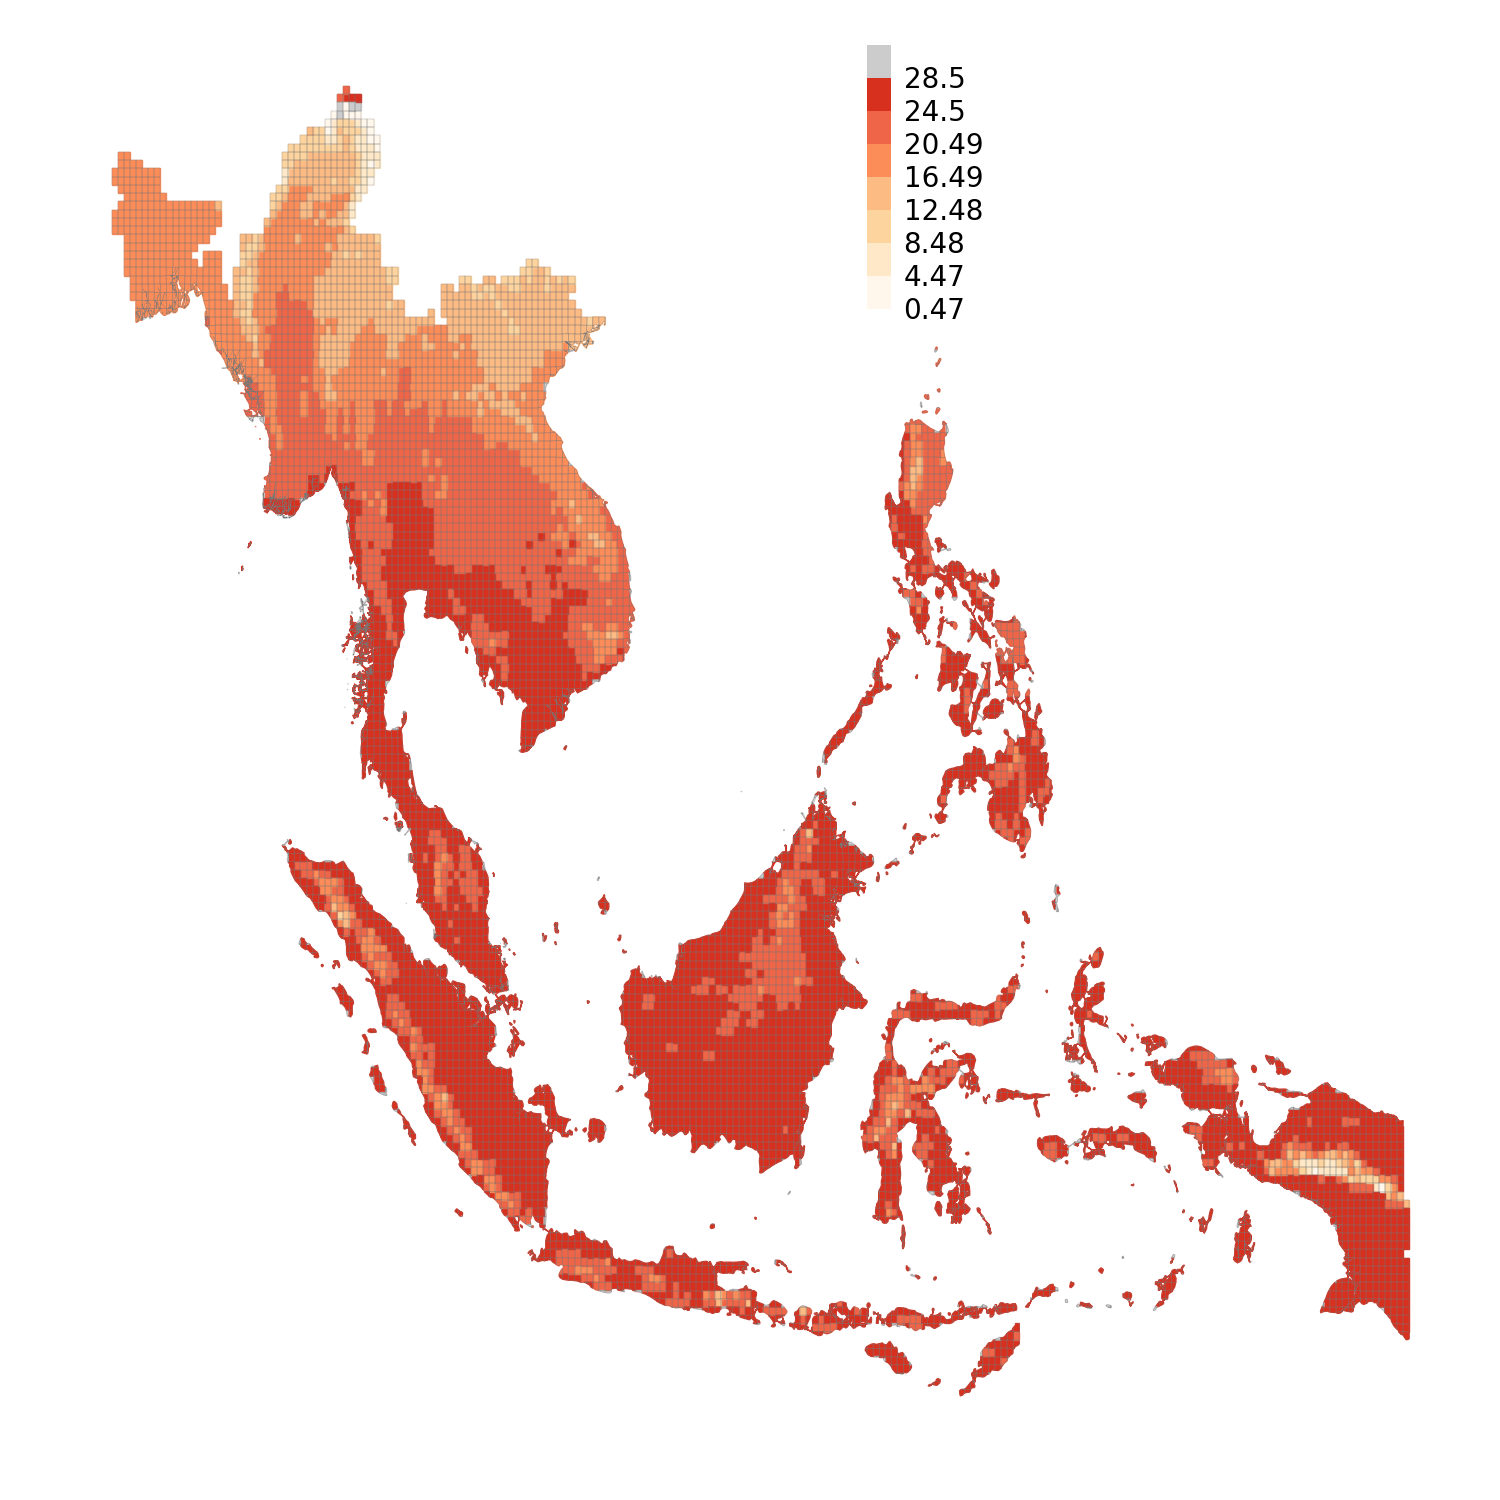
\includegraphics[width=\textwidth]{figs/heatmap_temp0.png}
%%         \caption{Temp Jan.}
%% \end{subfigure}
%% %
%% \begin{subfigure}[b]{.45\textwidth}
%%         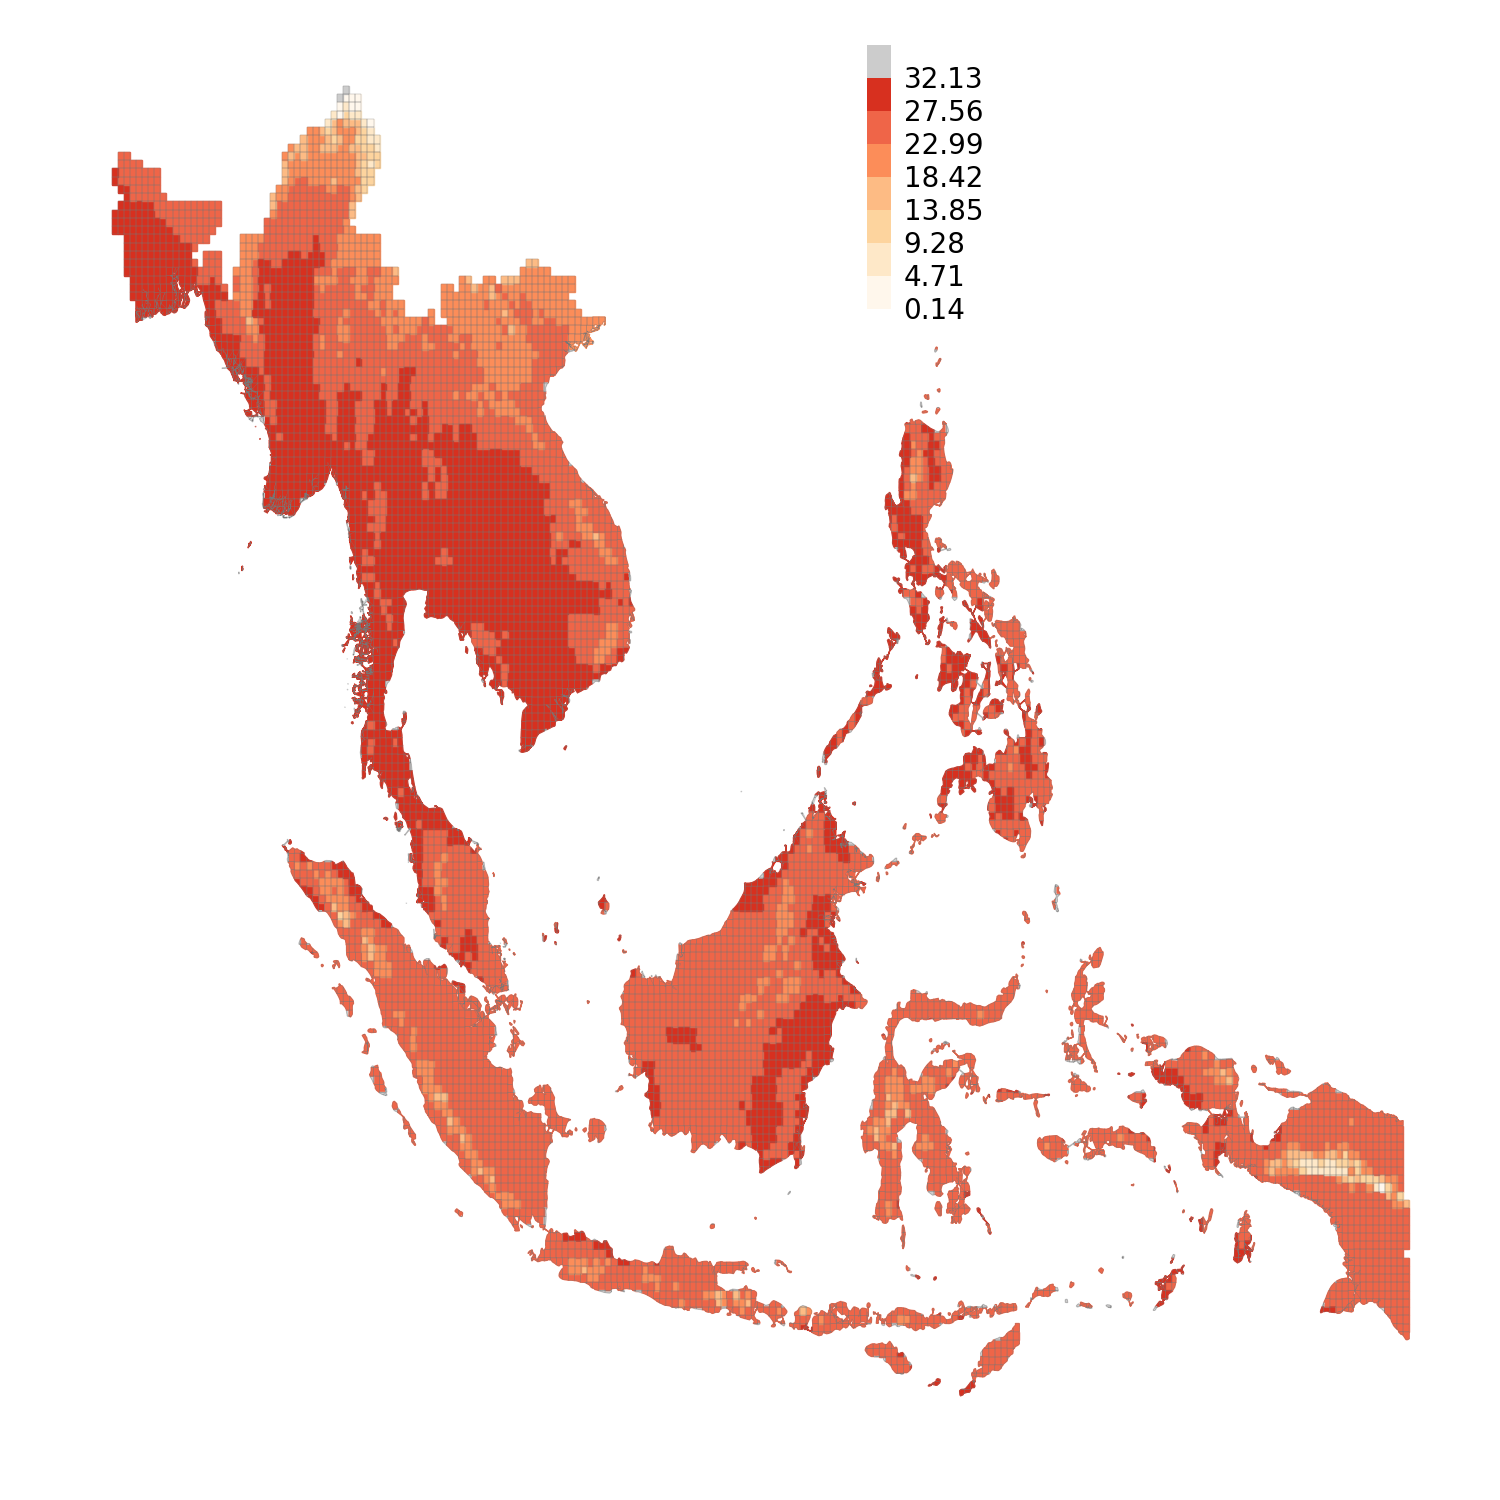
\includegraphics[width=\textwidth]{figs/heatmap_temp3.png}
%%         \caption{Temp Apr.}
%% \end{subfigure}
%% %
%% \begin{subfigure}[b]{.45\textwidth}
%%         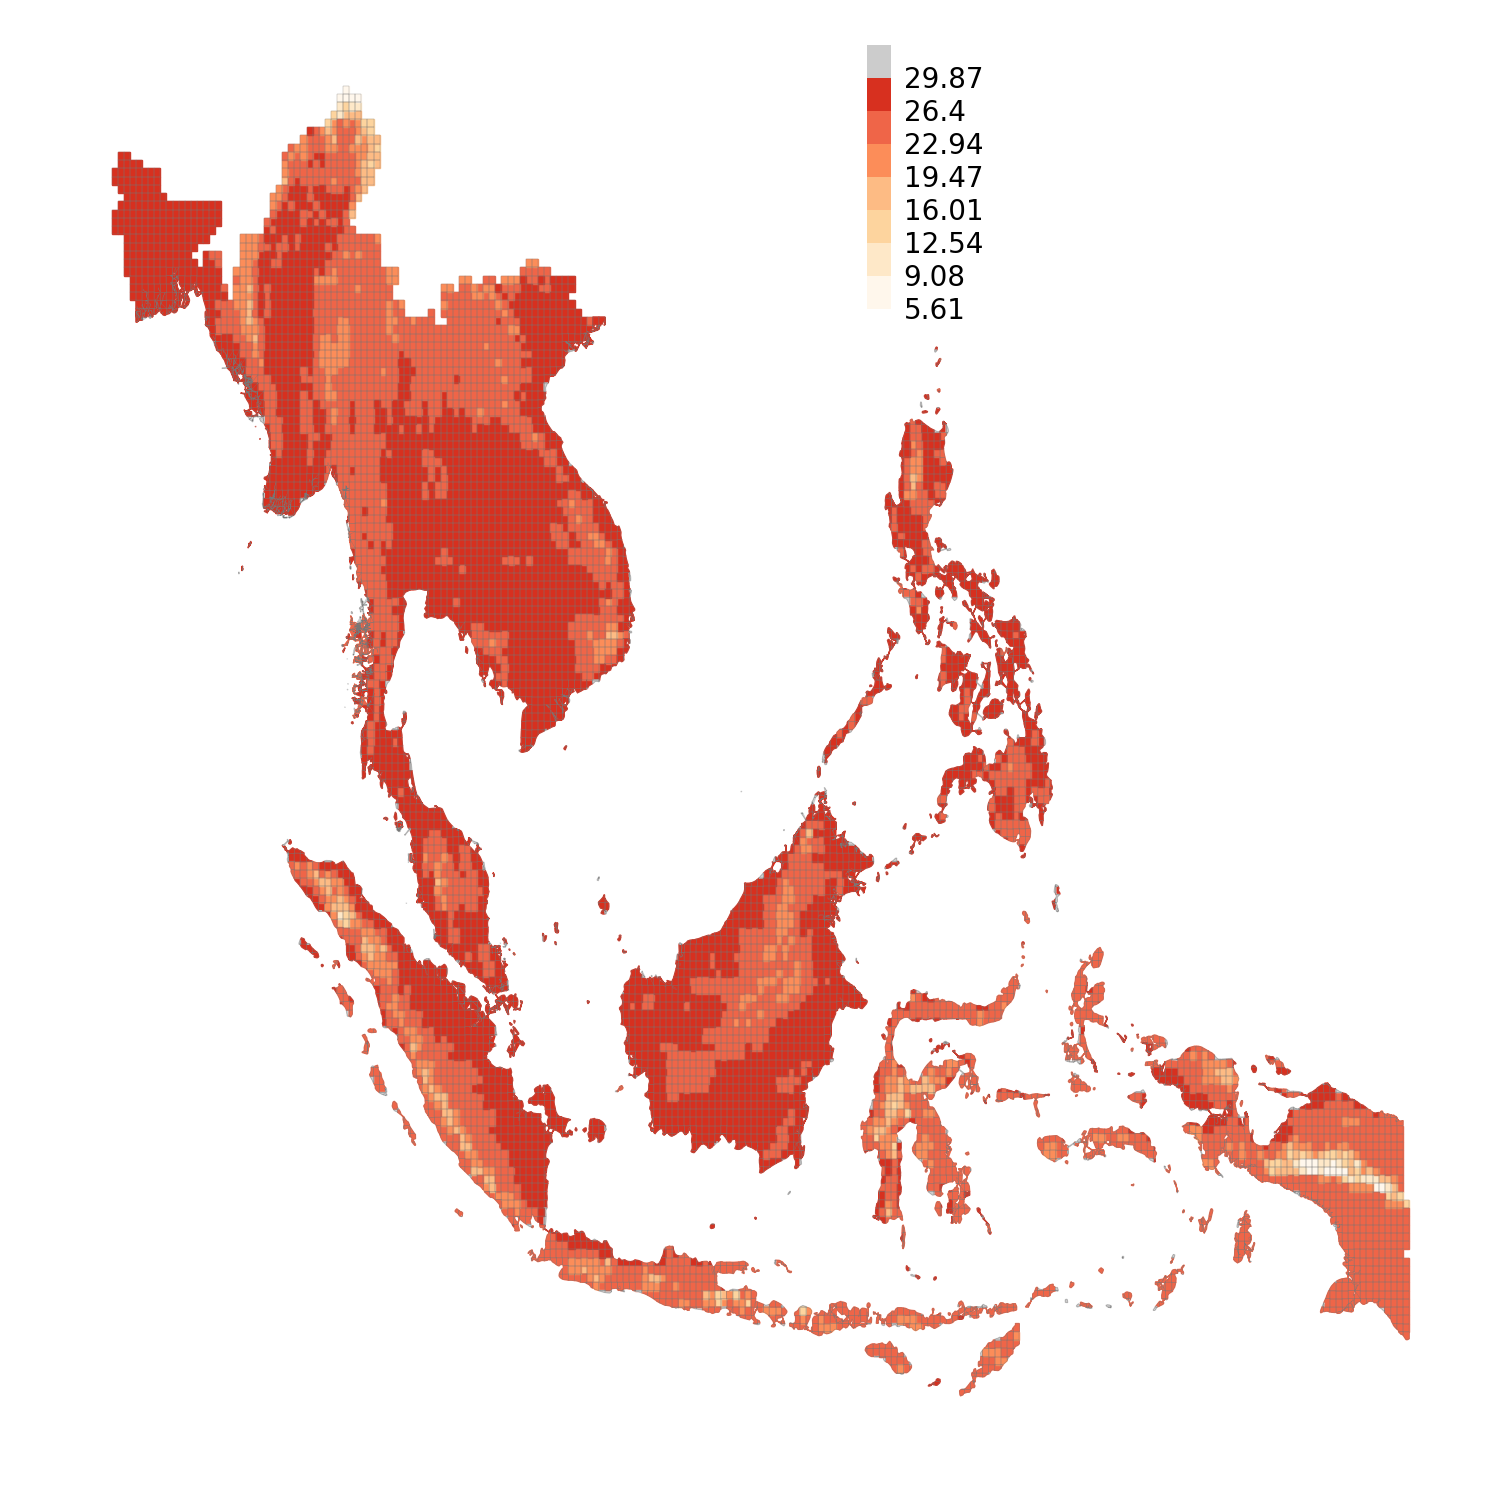
\includegraphics[width=\textwidth]{figs/heatmap_temp6.png}
%%         \caption{Temp July}
%% \end{subfigure}
%% %
%% \begin{subfigure}[b]{.45\textwidth}
%%         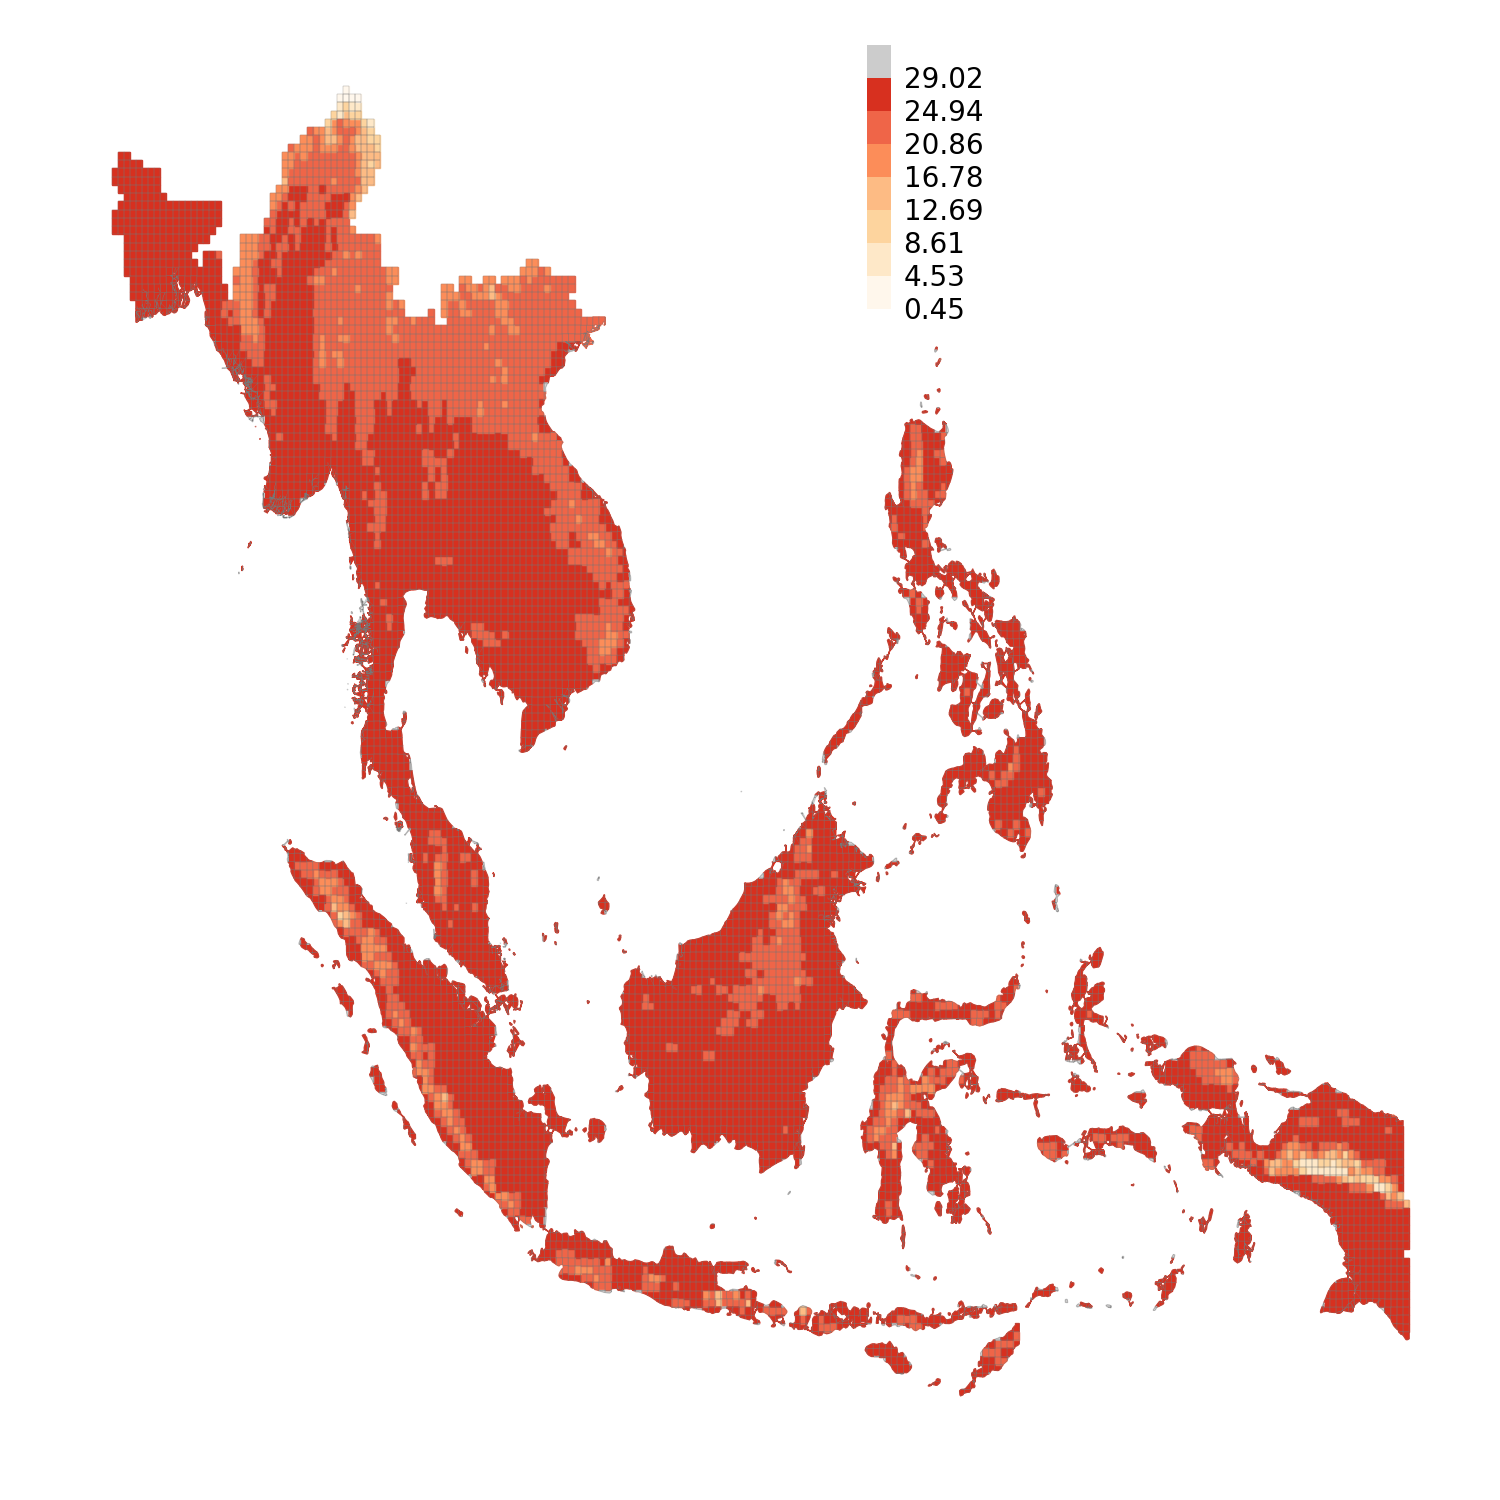
\includegraphics[width=\textwidth]{figs/heatmap_temp9.png}
%%         \caption{Temp Oct.}
%% \end{subfigure}
%% \caption{Data Plots}
%% \end{figure}
%% 
%%
 
%% \begin{figure}[ht]
%%     \centering
%% \begin{subfigure}[b]{.32\textwidth}
%%     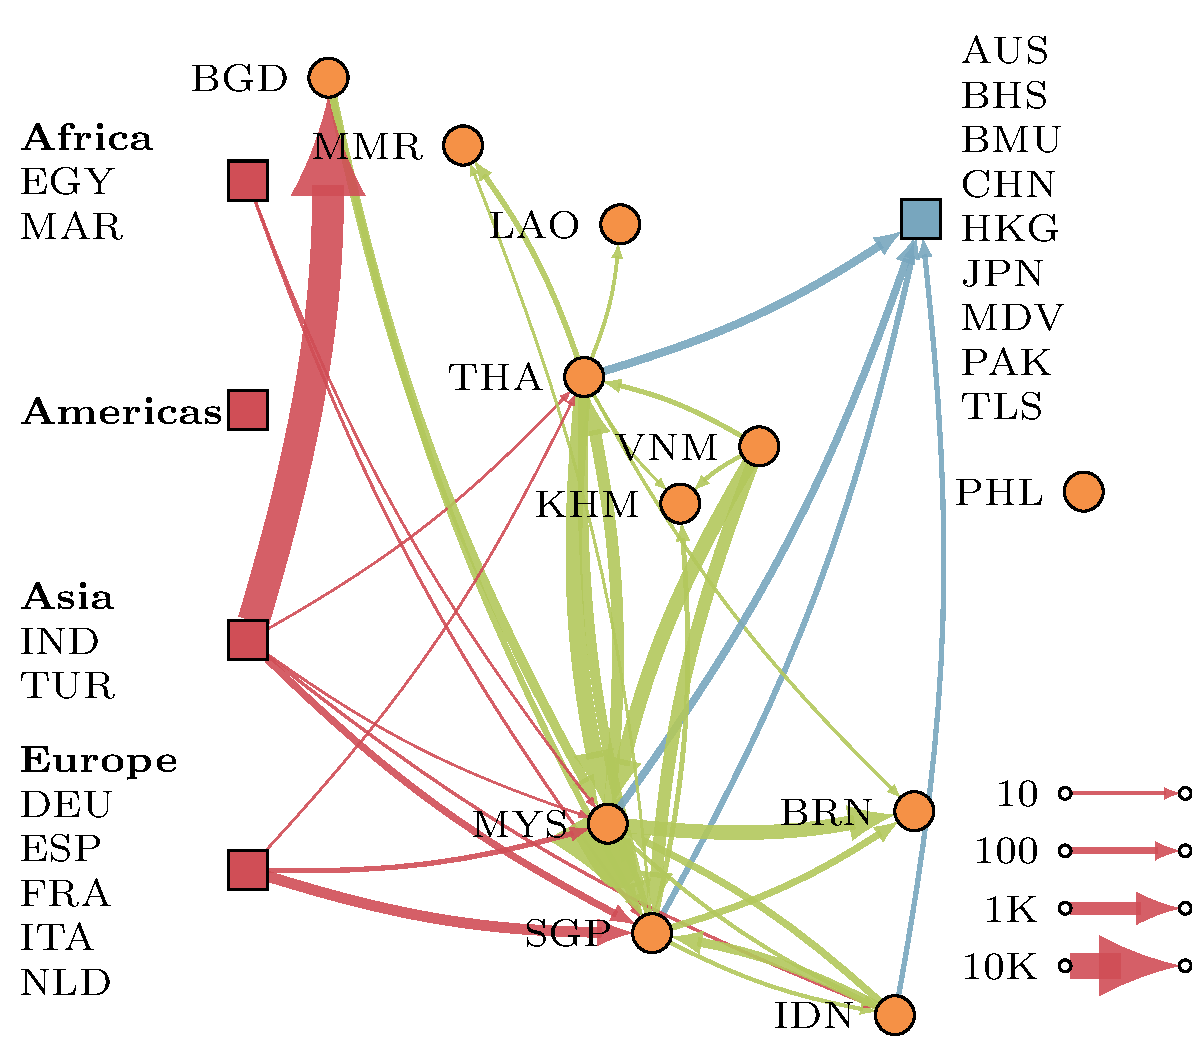
\includegraphics[width=\textwidth]{../international_trade/results/network_plots/sea_2013_tomato.pdf}
%%     \caption{Tomato}
%% \end{subfigure}
%% %%
%% \begin{subfigure}[b]{.32\textwidth}
%%     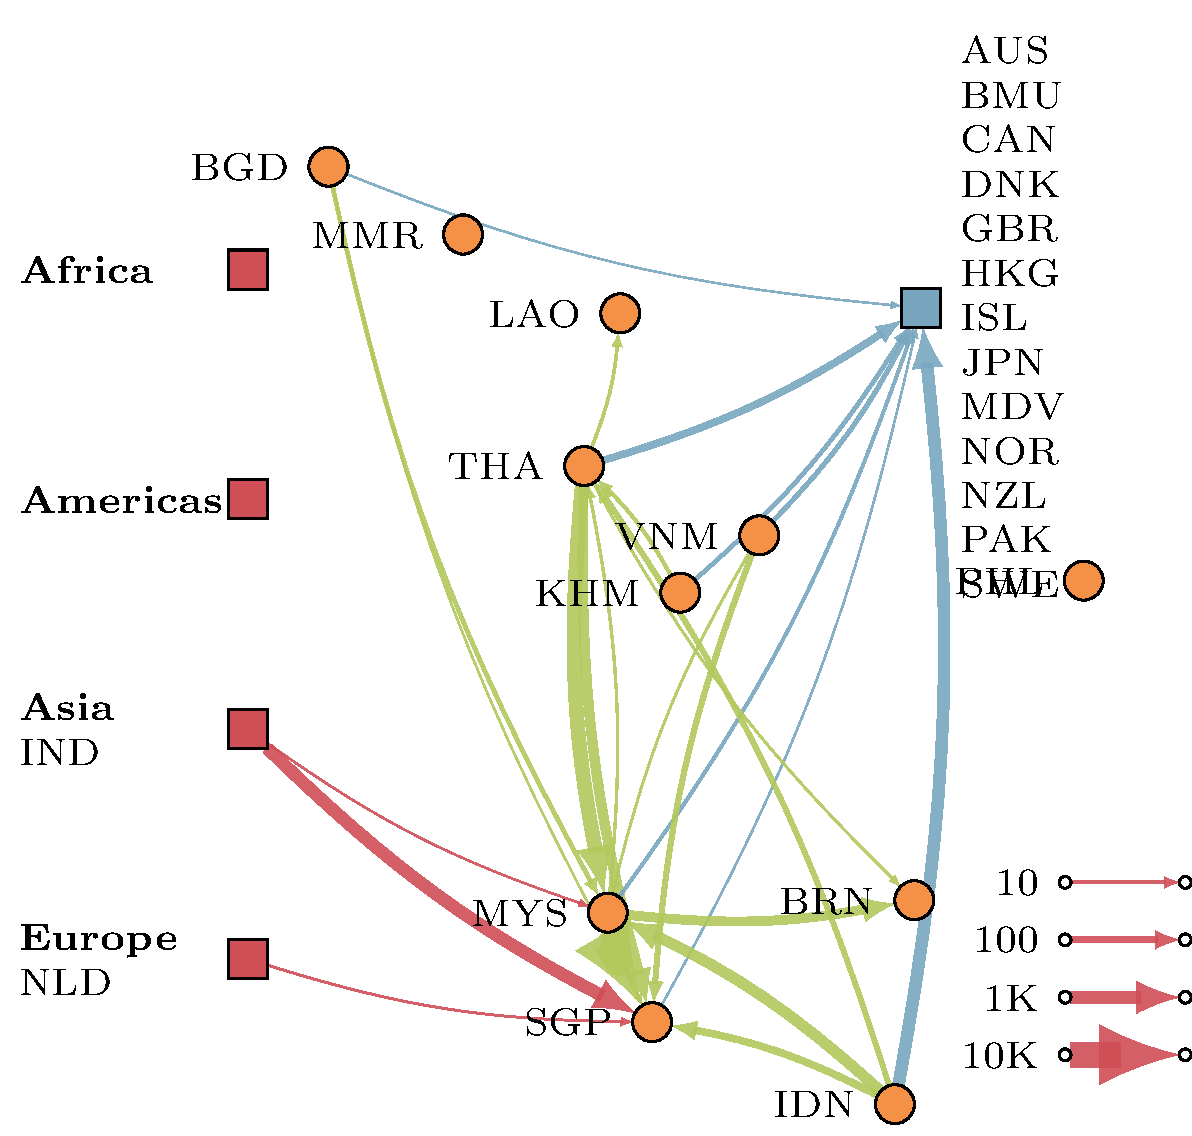
\includegraphics[width=\textwidth]{../international_trade/results/network_plots/sea_2013_eggplant.pdf}
%%     \caption{Eggplants}
%% \end{subfigure}
%%     %%
%% \begin{subfigure}[b]{.45\textwidth}
%%     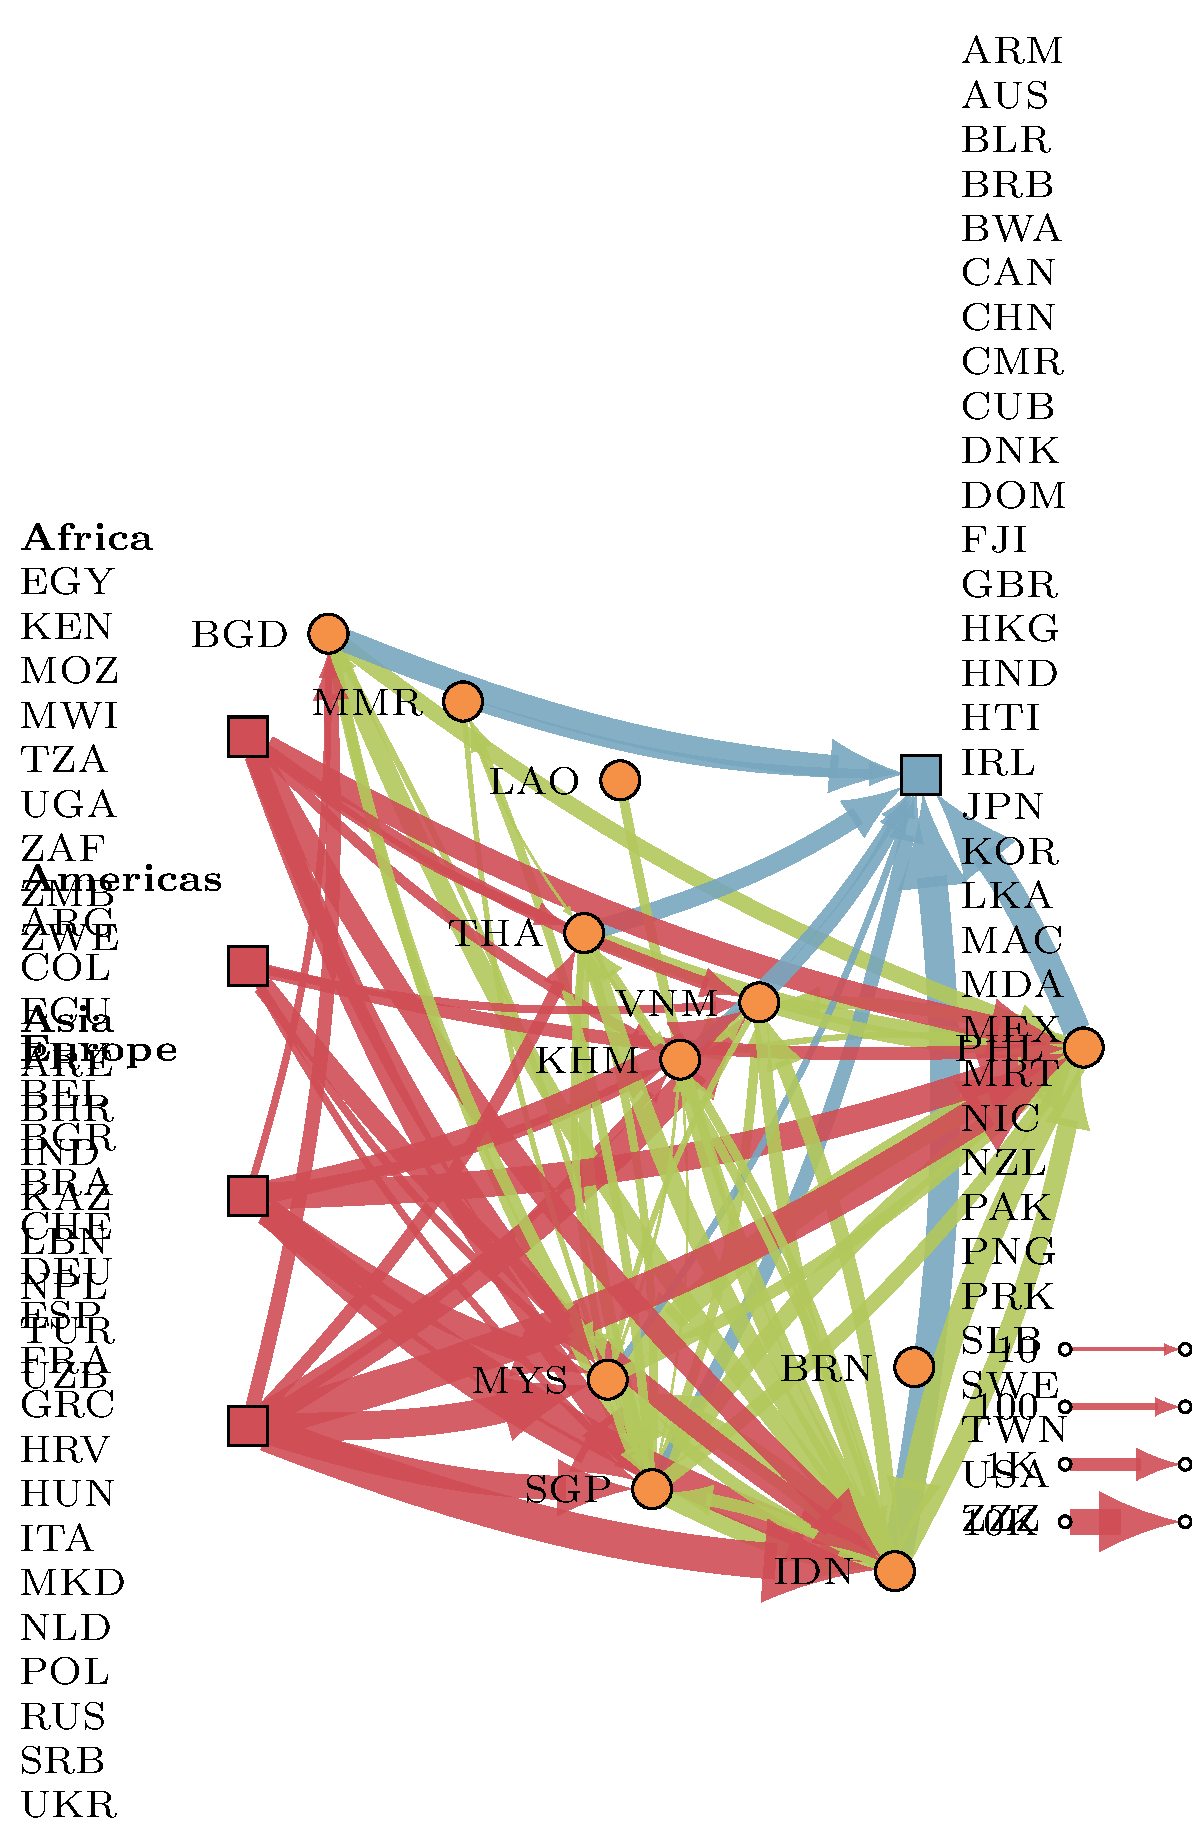
\includegraphics[width=\textwidth]{../international_trade/results/network_plots/sea_2013_tobacco.pdf}
%%     \caption{Tobacco 2013}
%% \end{subfigure}
    %%
%% \begin{subfigure}[b]{.45\textwidth}
%%     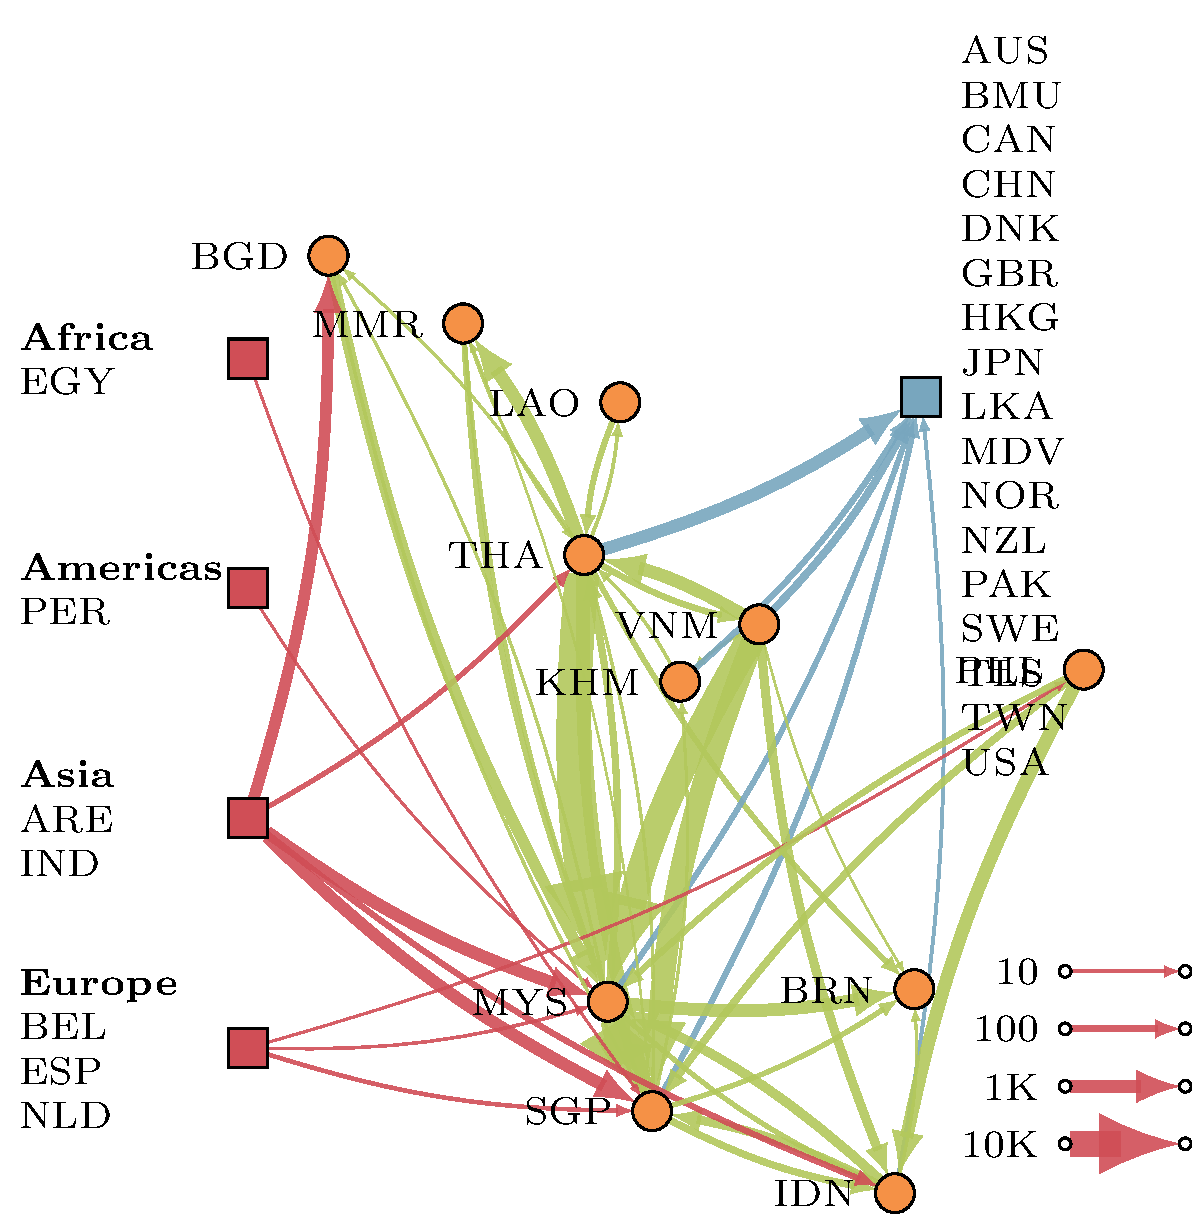
\includegraphics[width=\textwidth]{../international_trade/results/network_plots/sea_2013_pepper.pdf}
%%     \caption{Peppers 2013}
%% \end{subfigure}
    %%
%% \begin{subfigure}[b]{.32\textwidth}
%%     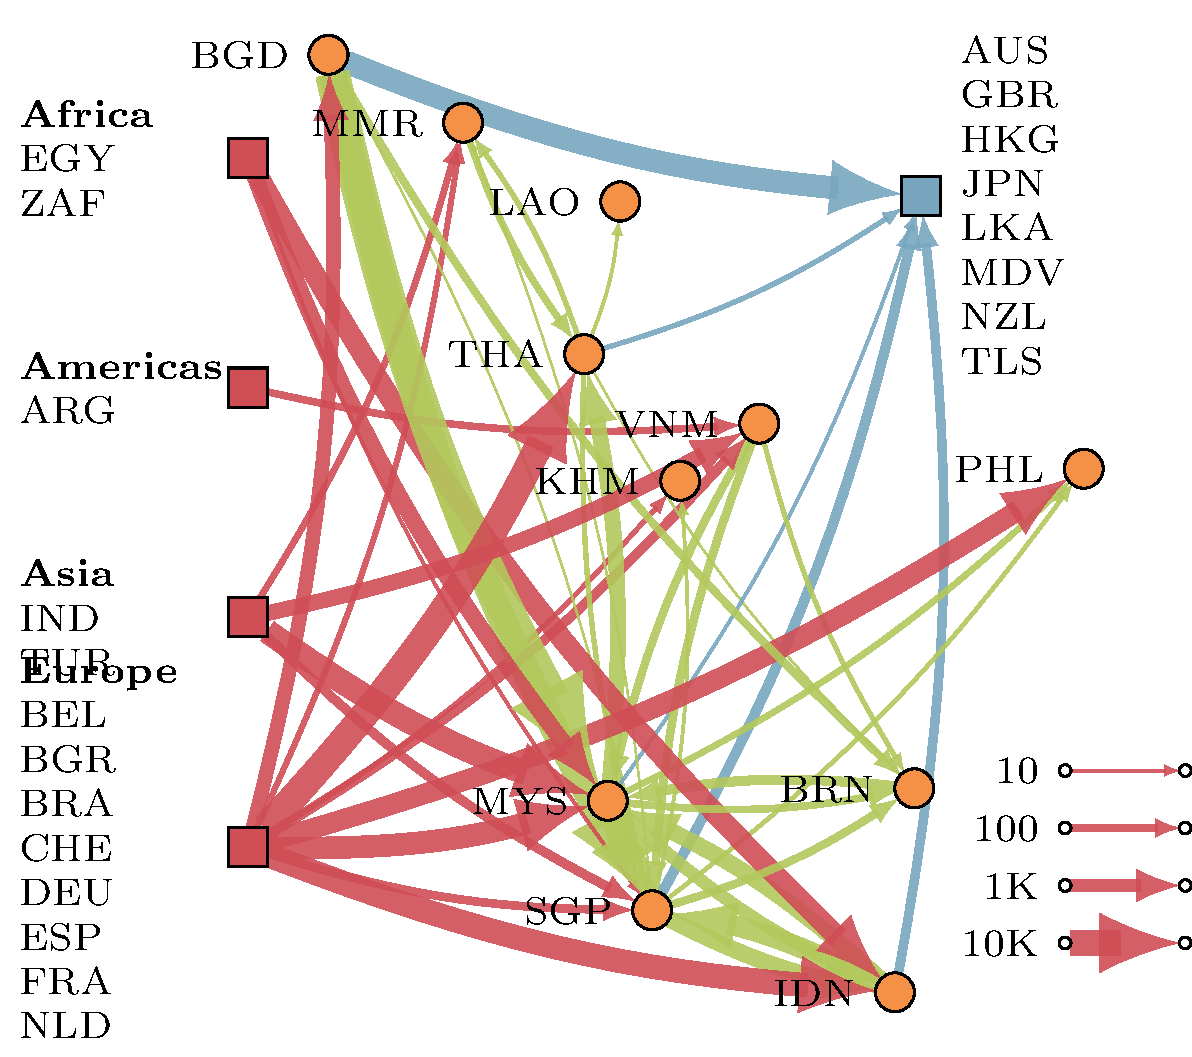
\includegraphics[width=\textwidth]{../international_trade/results/network_plots/sea_2013_potato.pdf}
%%     \caption{Potato}
%% \end{subfigure}
%% \caption{Trade networks for considered hosts of \tuta{} (year 2013).}
%% \end{figure}
%%
%%
\section{Multi-pathway Model}
\subsection{Locality construction}\label{sec:locality}
In the model, \emph{localities} are centres of consumption or production.
From the perspective of consumption, we selected cities with population
greater than a certain population threshold (as per~\cite{maxmind}) in the
entire study region. The number and size of localities is controlled by
population threshold and locality radius parameters. We considered a range
of threshold values, and chose~$250,000$ as the threshold for the model
with the main criterion for the choice being coverage of population and
knowledge of major wholesale markets
(Figure~\ref{fig:localityConstruction}). Then, we added major production
centres if their population did not meet the threshold. The locality radius
was chosen to be~$100$km since local production in an urban area was
within 50--60km from the city centre for several countries in this
region~\cite{buntong2013,sokhen2004vegetable,wijk2007}. To obtain long
distance trade flows, the travel times between pairs of cities were
computed using Google API~\cite{googleapi}.
%%
\begin{figure}[t]
\centering
\begin{subfigure}[b]{.47\textwidth}
    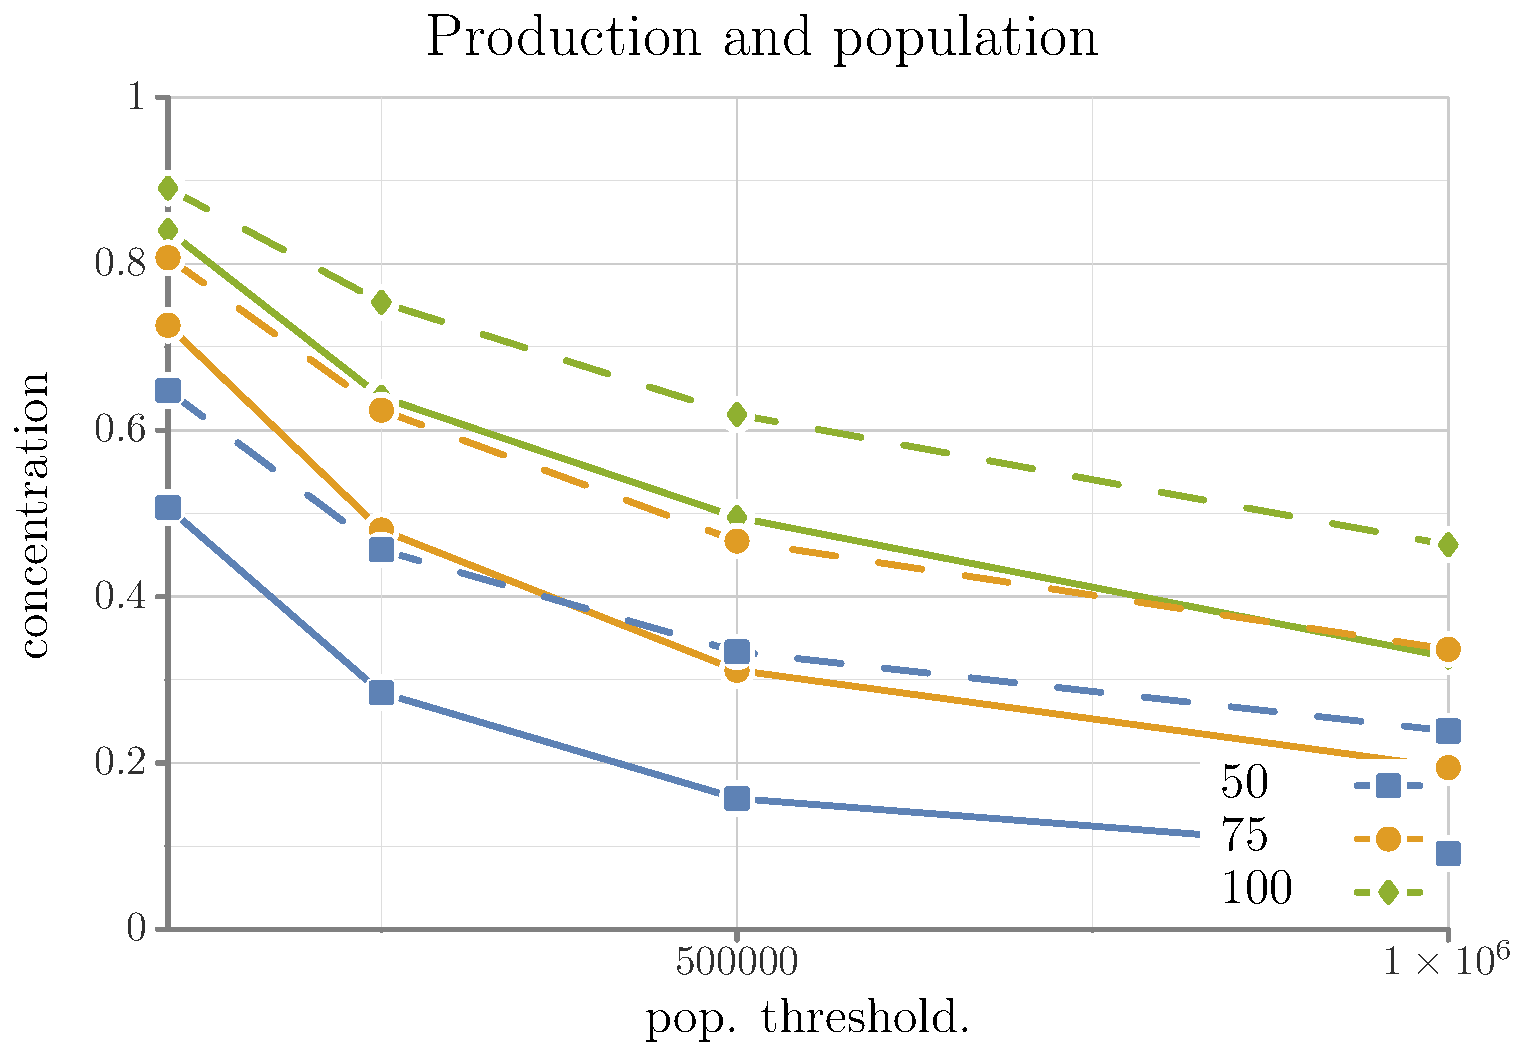
\includegraphics[width=\textwidth]{../cellular_automata/results/cities/concentration_with_popthresh.pdf}
\caption{}
\end{subfigure}
%%
\begin{subfigure}[b]{.47\textwidth}
    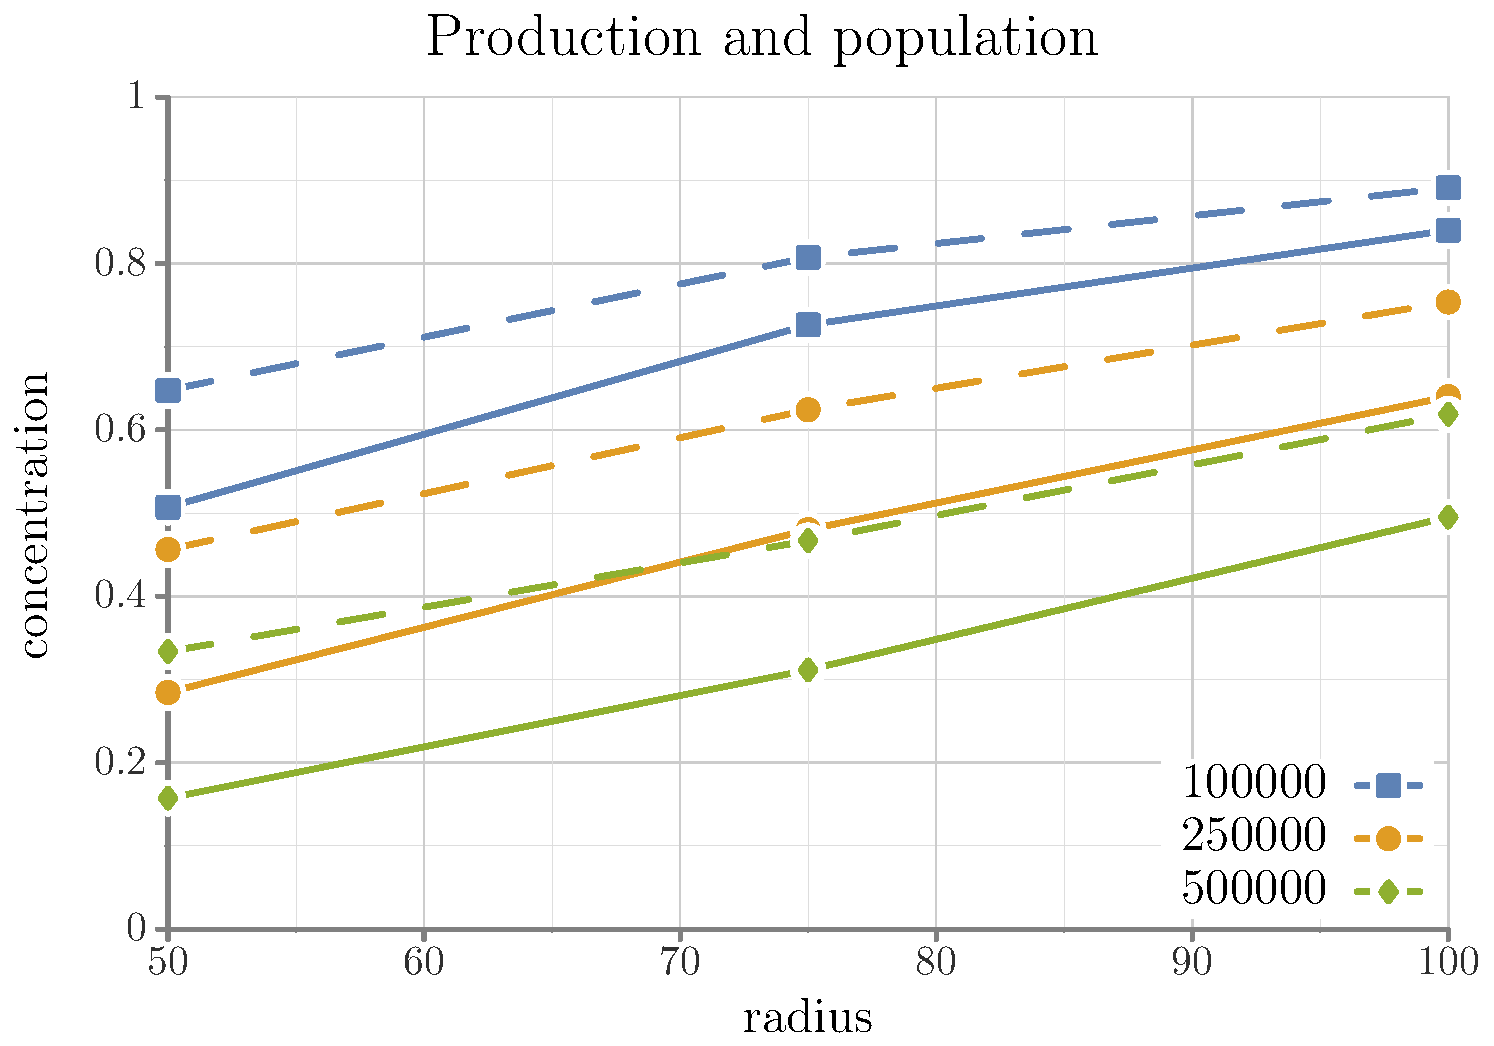
\includegraphics[width=\textwidth]{../cellular_automata/results/cities/concentration_with_radius.pdf}
\caption{}
\end{subfigure}
\caption{\textbf{Locality construction.} The number of localities and the
locality area is controlled by population threshold and locality radius. We
analysed the effect of these parameters on the amount of production and
population captured in the region. Setting a threshold of 250,000 and
radius of 100km, 80\% of the production and population is covered by
localities. \label{fig:localityConstruction}}
\end{figure}
%%
%% 
%% \begin{table}[!ht]
%% \caption{Market distances\label{tab:marketDist}}
%% \centering
%% \rowcolors{1}{white}{gray!15} % For this to work, put \PassOptionsToPackage{table}{xcolor} before \documentclass
%% \begin{tabular}{*{4}{c}}
%% \toprule
%% {city} & \parbox{3cm}{max. distance (kms) reported} & country & source \\
%% \midrule
%% Phnom Penh & 65 & Cambodia & \cite{buntong2013,sokhen2004vegetable} \\
%% Hanoi & 50 & Vietnam & \cite{wijk2007} \\
%% Vientiane & 50 & Laos & \cite{kethonga2004} \\
%% West Java & & Indonesia & \cite{kethonga2004} \\
%% \bottomrule
%% \end{tabular}
%% \end{table}
%%

\subsection{Seasonal production}\label{sec:prod} 
We estimated monthly production volume of tomato, eggplant and potato for
each cell using production data available at the country/state/province
level and the Spatial Production Allocation Model~\cite{spam}. The latter
uses a generalised cross-entropy approach to allocate crop production in
administrative units into individual pixels, through judicious
interpretation of all accessible evidence such as production statistics,
farming systems, satellite image, crop biophysical suitability, crop price,
local market access and prior knowledge. The monthly production volume was
estimated in two steps: (i)~Estimation of cell-level annual production, and
(ii)~disaggregation of annual production to monthly production.

\paragraph{Annual production.} From SPAM~\cite{spam}, we obtained annual
production estimates for each cell.  However, there are several issues with
directly using this data. Firstly, these are estimates for the year~$2005$,
and secondly, tomato and eggplant production estimates are not available.
Instead, total vegetable production volume is available. Also, for
countries where data was available, we did not find any correlation between
reported tomato (eggplant) production and total SPAM vegetable production
for that region. Therefore, for each country, we obtained the most recent
production data available (2013 or later) at the highest spatial resolution
(region/province/country) (Table~S1). The production of a particular
vegetable type at a cell was computed as follows:
%%
\[\frac{\text{Total production in the region}}{\text{Total SPAM production
    for cells in the region}}\times \text{SPAM production in the cell} \;.\]
%%
For tomato and eggplant, we used vegetable production as the surrogate.
There were also cases where no data was available (Cambodia, Myanmar and
Laos for example). In such cases, for potato, we used SPAM data as is. For
tomato and eggplant, the SPAM value for vegetables was scaled by a scaling
factor which was determined as follows. For countries where data was
available, we computed the ratio of total tomato production and total SPAM
vegetable production for the country. The median value ($\approx0.05$) was
used as the scaling factor. The same procedure was used for eggplant. 

\paragraph{Monthly production.} In order to estimate the seasonal production rates of tomatoes, we
considered quarterly production data from Philippines~\cite{psa2017} for the 16
regions of the country and studied its relationship between precipitation,
elevation and temperature. We first assigned average monthly precipitation,
temperature and elevation data to the cells by latitude and longitude.
Next, for each region, we obtained the seasonal relative tomato production
(or production rate). This was obtained by dividing each of the quarterly
production volume by total annual production volume. We conducted a linear
regression with the product rate as a dependent variable and the
precipitation as an independent variable in SPSS 24.0. Since the dependent
variable was highly skewed, we implemented a log-transformation for it. To
control elevation, we classified the elevations into two groups, high and
low, using K means in SPSS 24.0. Due to the small sample size, we excluded
the samples in the high-elevation group and conducted a linear regression
analysis for the group of low elevation ($< 235$). 

The regression results showed that precipitation was a statistically
significant predictor ($p <0.001$, $R^2=0.54$). When we accounted for
temperature along with precipitation, the~$R$ value increased to $0.58$
with temperature exhibiting weak correlation with production.  Though the
results with both variables included gave a slightly stronger correlation,
in the validation step, the regression function corresponding to
precipitation was a better match for the rest of the study region. Thus we
decided to use only precipitation as a predictor for seasonality of tomato
production. Table~\ref{fig:regression} provides information on these
regression results.

\begin{table}[!ht]
    \centering
	\small
    \caption{Linear regression results for seasonal production as a
        function of precipitation.
        \label{fig:regression}}
    \begin{tabular}{c c c c c c}
		\hline	 	
		 & B & Std. Error & Beta & t & Sig.  \\
		\hline		
		\hline
        Intercept & -0.208 & 0.229 & & -0.908 & 0.368 \\
        \hline
        Precipitation & -0.008 & 0.001 & -0.734 & -7.935 & 0.000 \\
    \end{tabular}
\end{table}

\paragraph{Validation.} With the exception of data from Philippines on
tomato and eggplant, there is no regional seasonal production information
for the three crops considered for other countries.  However, there are
several reports that provide qualitative information. See
Table~\ref{tab:countryData}, column ``Seasons''. In some cases seasonal
production data is available at the country level. For example, for
Bangladesh, eggplant production volume is available by season. Similar
information is available for Cambodia. In Figure~\ref{fig:seasonalProd}, we
have compared seasonal production predicted by the regression model with available
qualitative and quantitative information. We note that the precipitation
based regression function captures the general trend of seasonal production
in the different regions considered.

\begin{figure}[!ht]
\centering
\begin{subfigure}[b]{.32\textwidth}
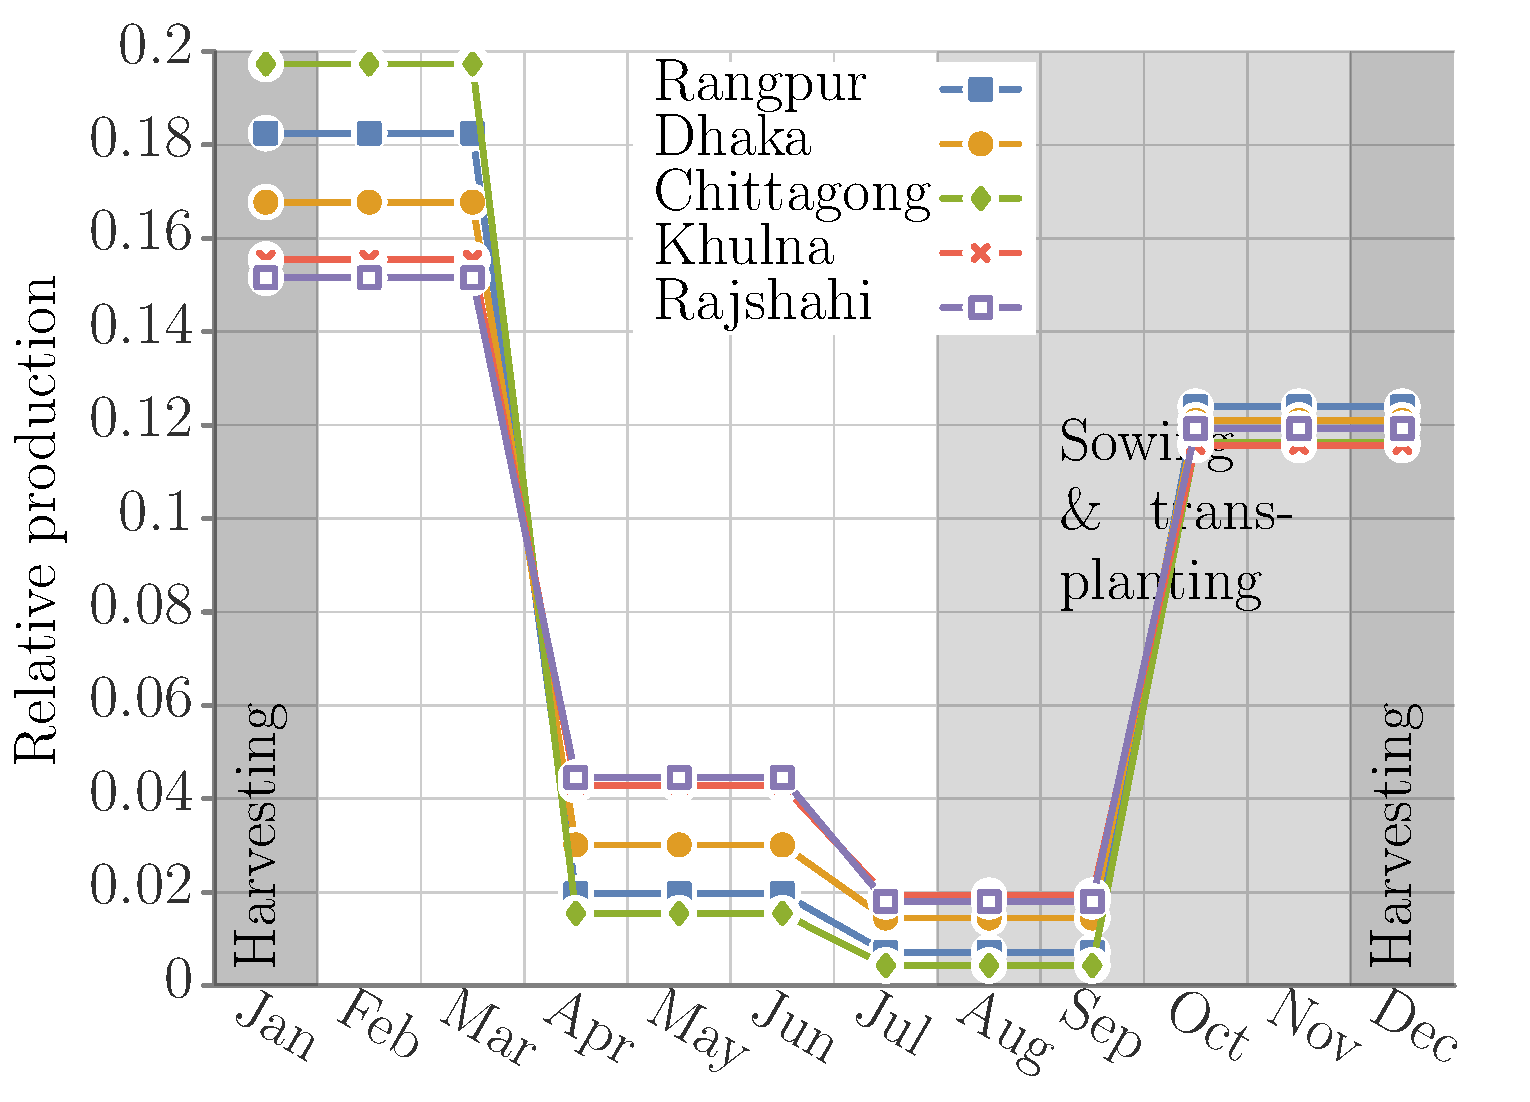
\includegraphics[width=\textwidth]{../production/results/prod_tomato_BGD.pdf}
\caption{Bangladesh tomato production compared with growing season
    information~\cite{bbs2017}}
\end{subfigure}
\begin{subfigure}[b]{.32\textwidth}
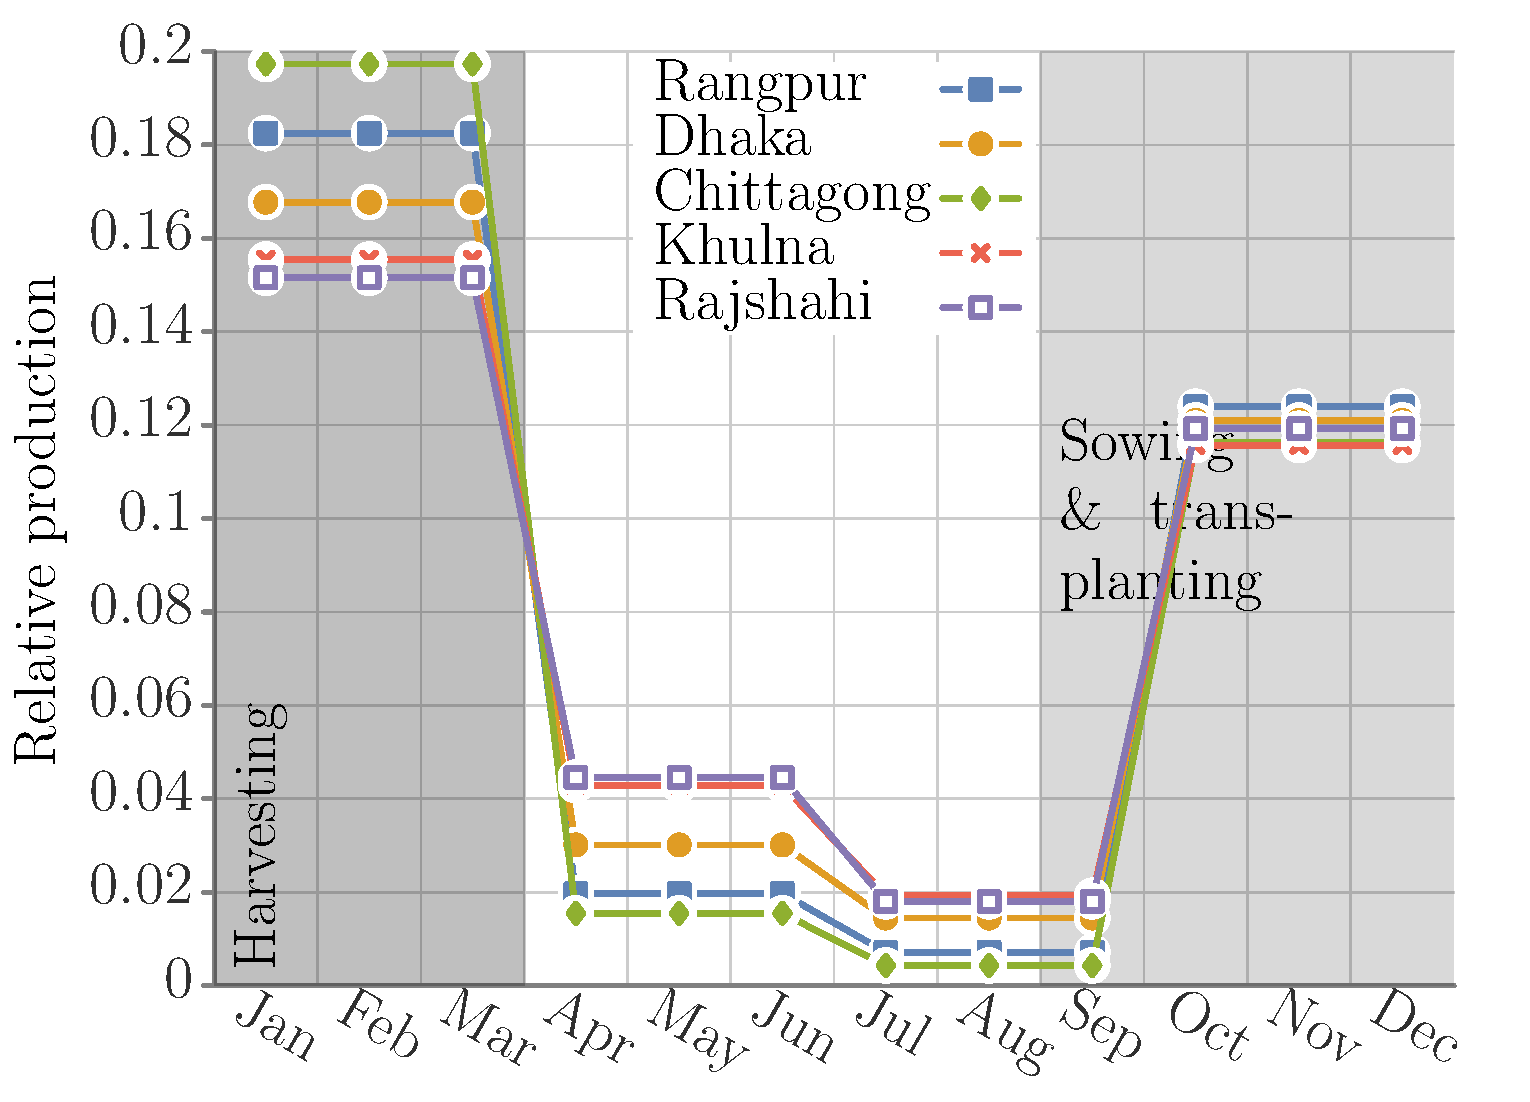
\includegraphics[width=\textwidth]{../production/results/prod_potato_BGD.pdf}
\caption{Bangladesh potato production compared with growing season
    information~\cite{bbs2017}}
\end{subfigure}
\begin{subfigure}[b]{.32\textwidth}
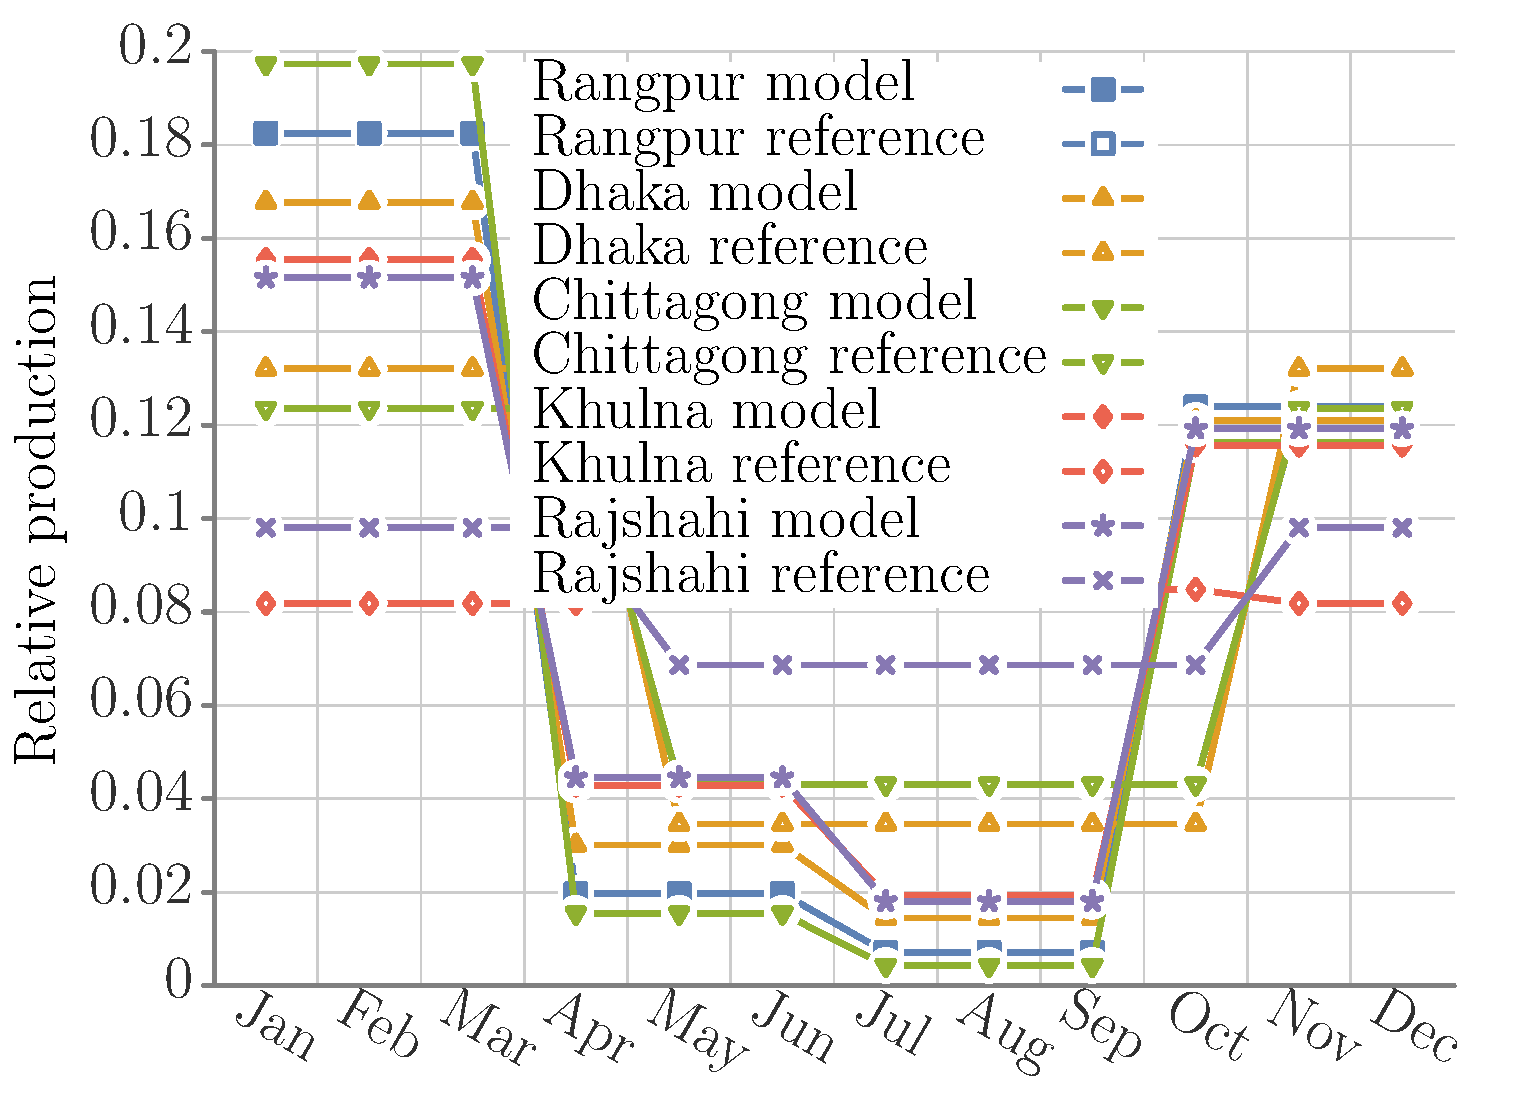
\includegraphics[width=\textwidth]{../production/results/prod_eggplant_BGD.pdf}
\caption{Bangladesh eggplant production compared with growing season
    information~\cite{bbs2017}}
\end{subfigure}
\begin{subfigure}[b]{.32\textwidth}
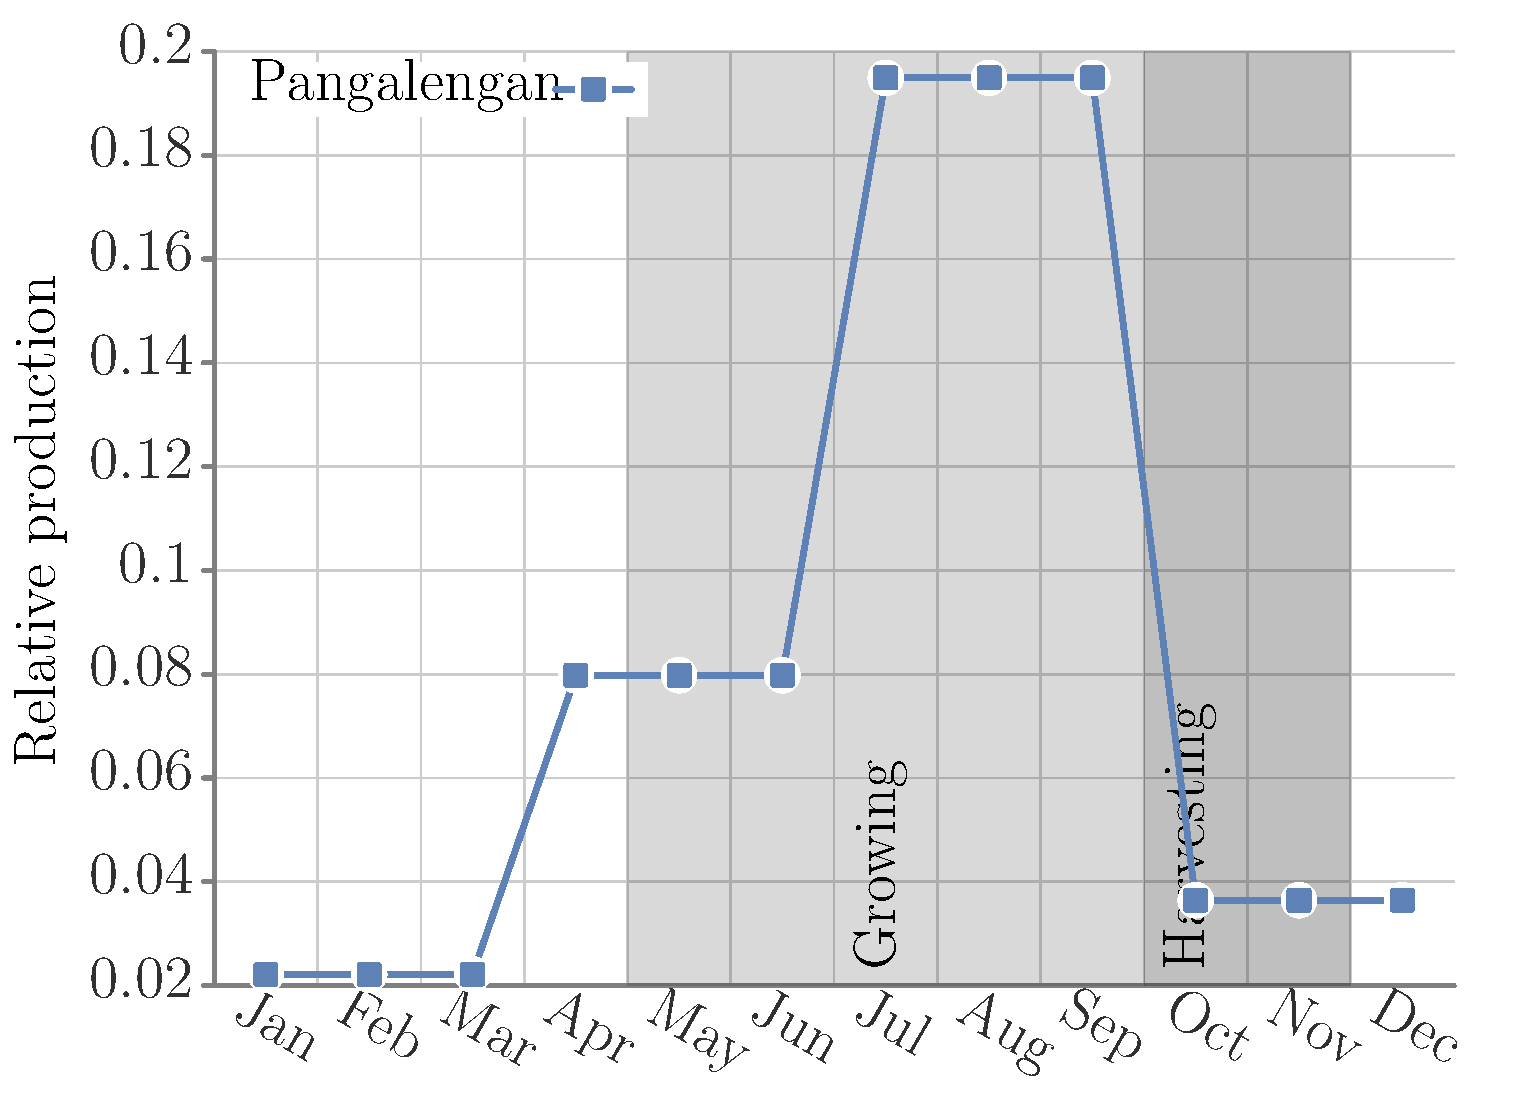
\includegraphics[width=\textwidth]{../production/results/prod_tomato_IDN.pdf}
\caption{Indonesia tomato production compared with growing season
    information~\cite{arsanti2015}}
\end{subfigure}
\begin{subfigure}[b]{.32\textwidth}
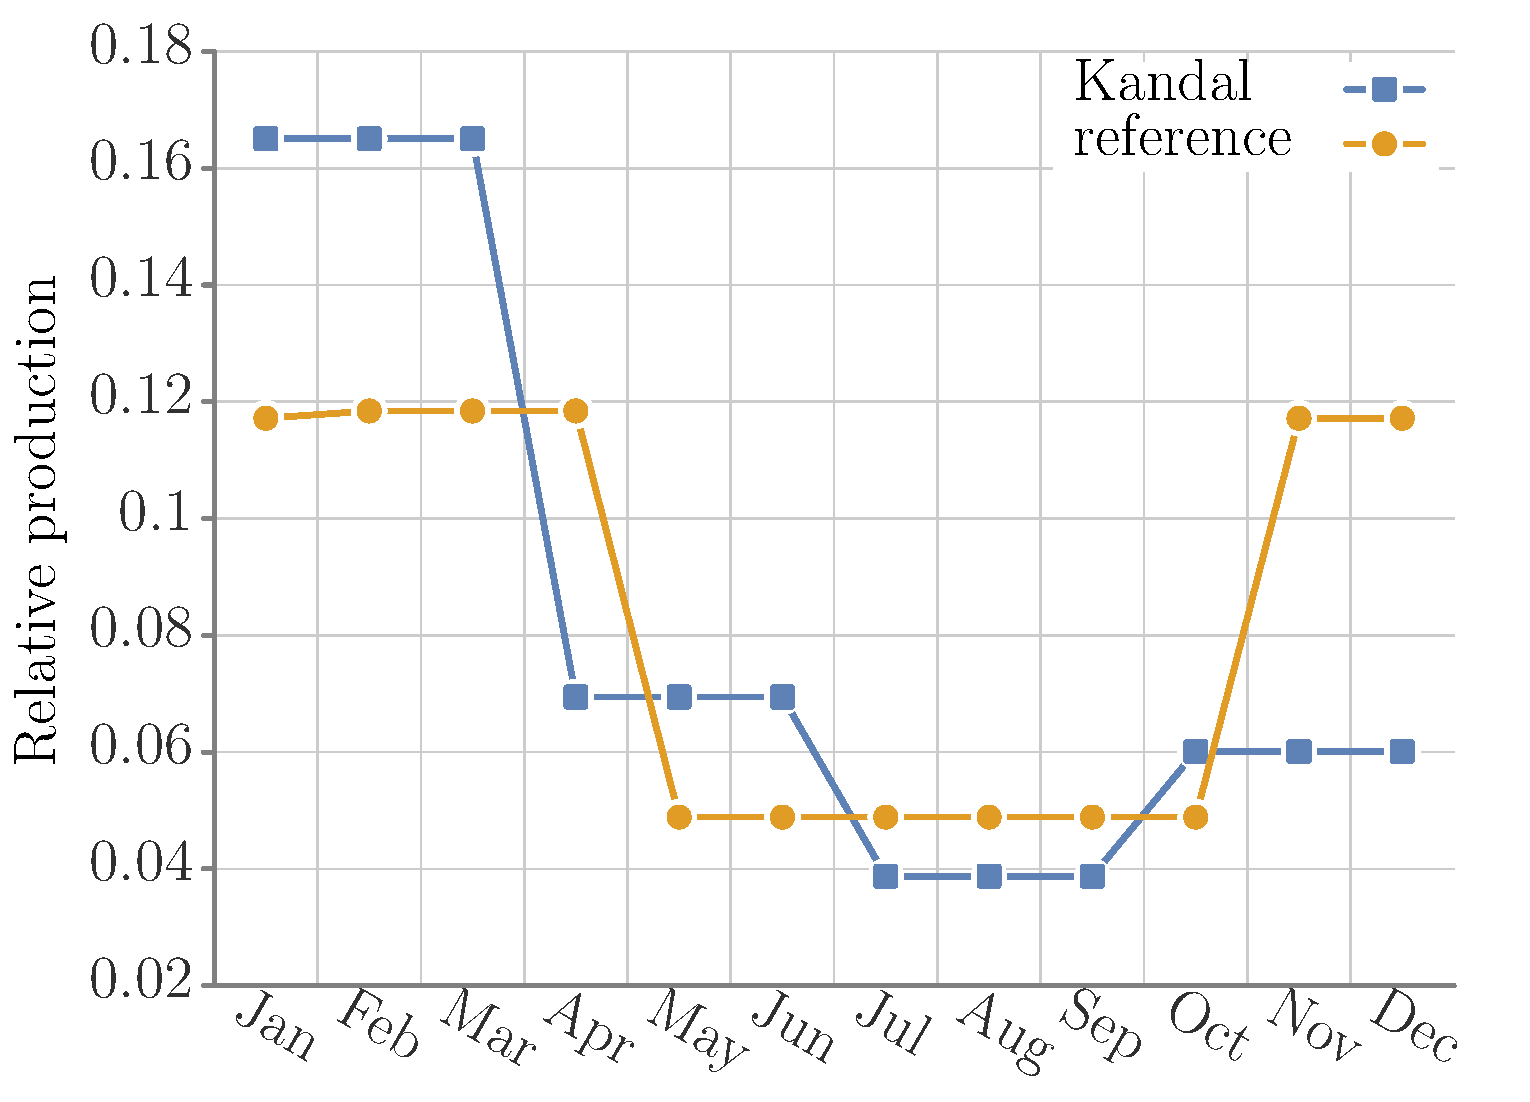
\includegraphics[width=\textwidth]{../production/results/prod_tomato_KHM.pdf}
\caption{Cambodia tomato production compared with seasonal production
    information~\cite{genova2006postharvest}}
\end{subfigure}
\begin{subfigure}[b]{.32\textwidth}
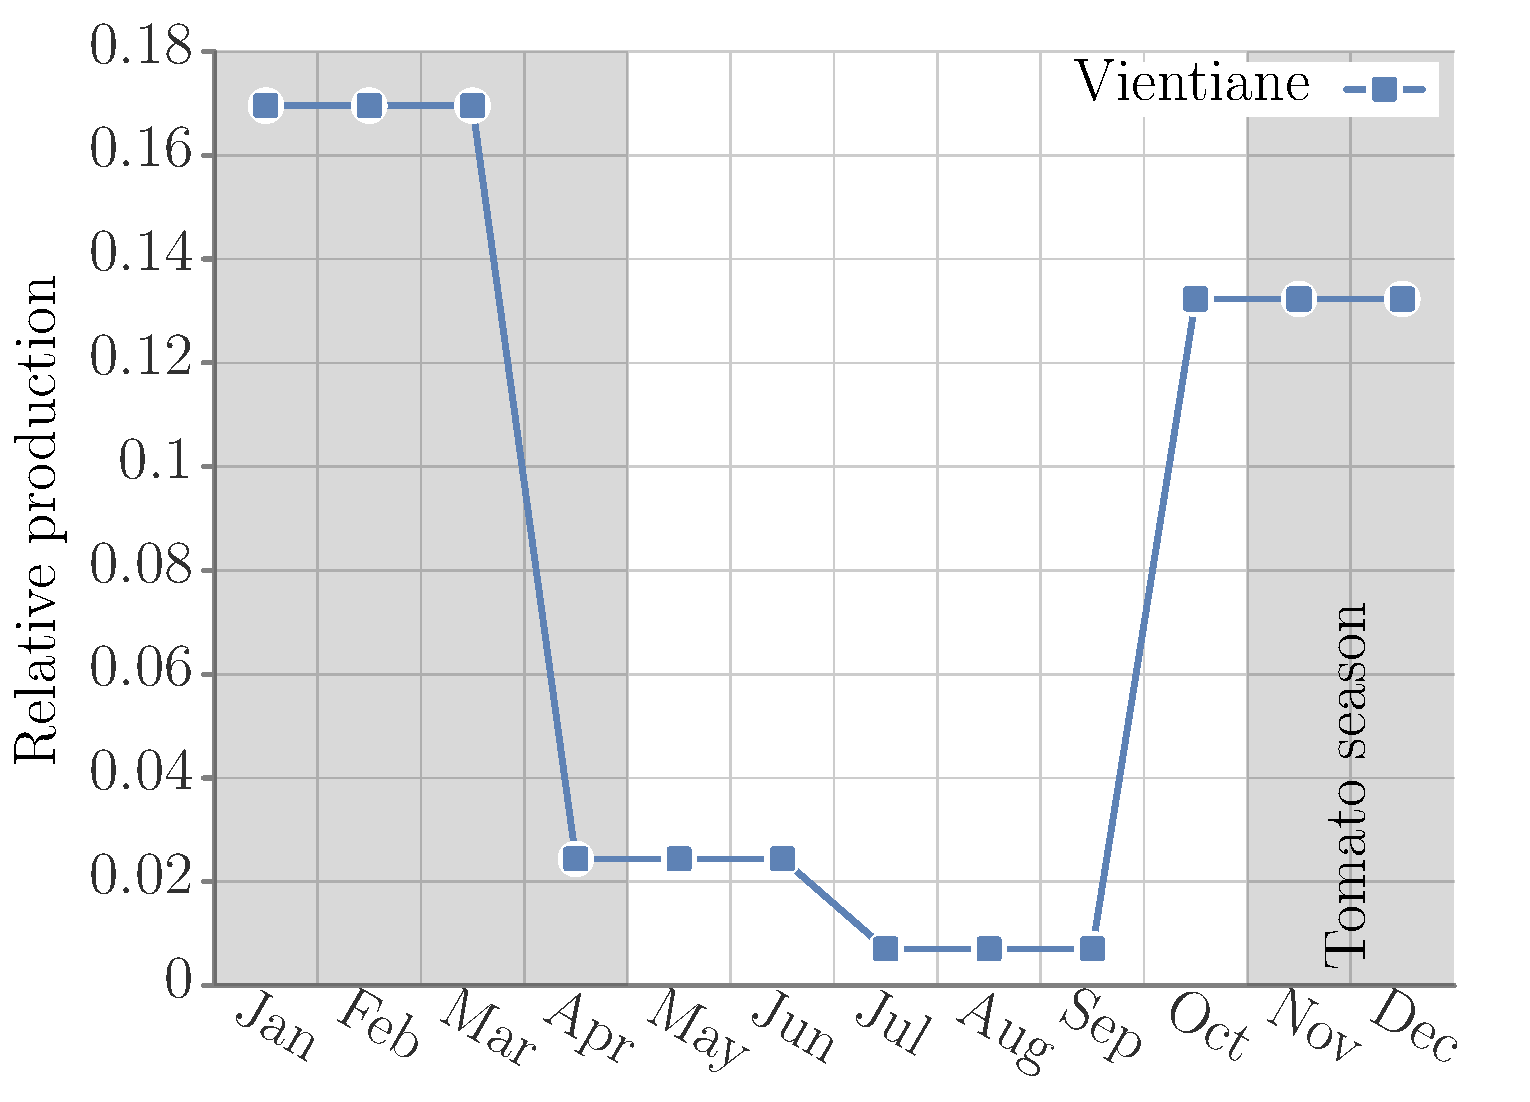
\includegraphics[width=\textwidth]{../production/results/prod_tomato_LAO.pdf}
\caption{Laos tomato production compared with growing season
    information~\cite{kethonga2004}}
\end{subfigure}
\begin{subfigure}[b]{.32\textwidth}
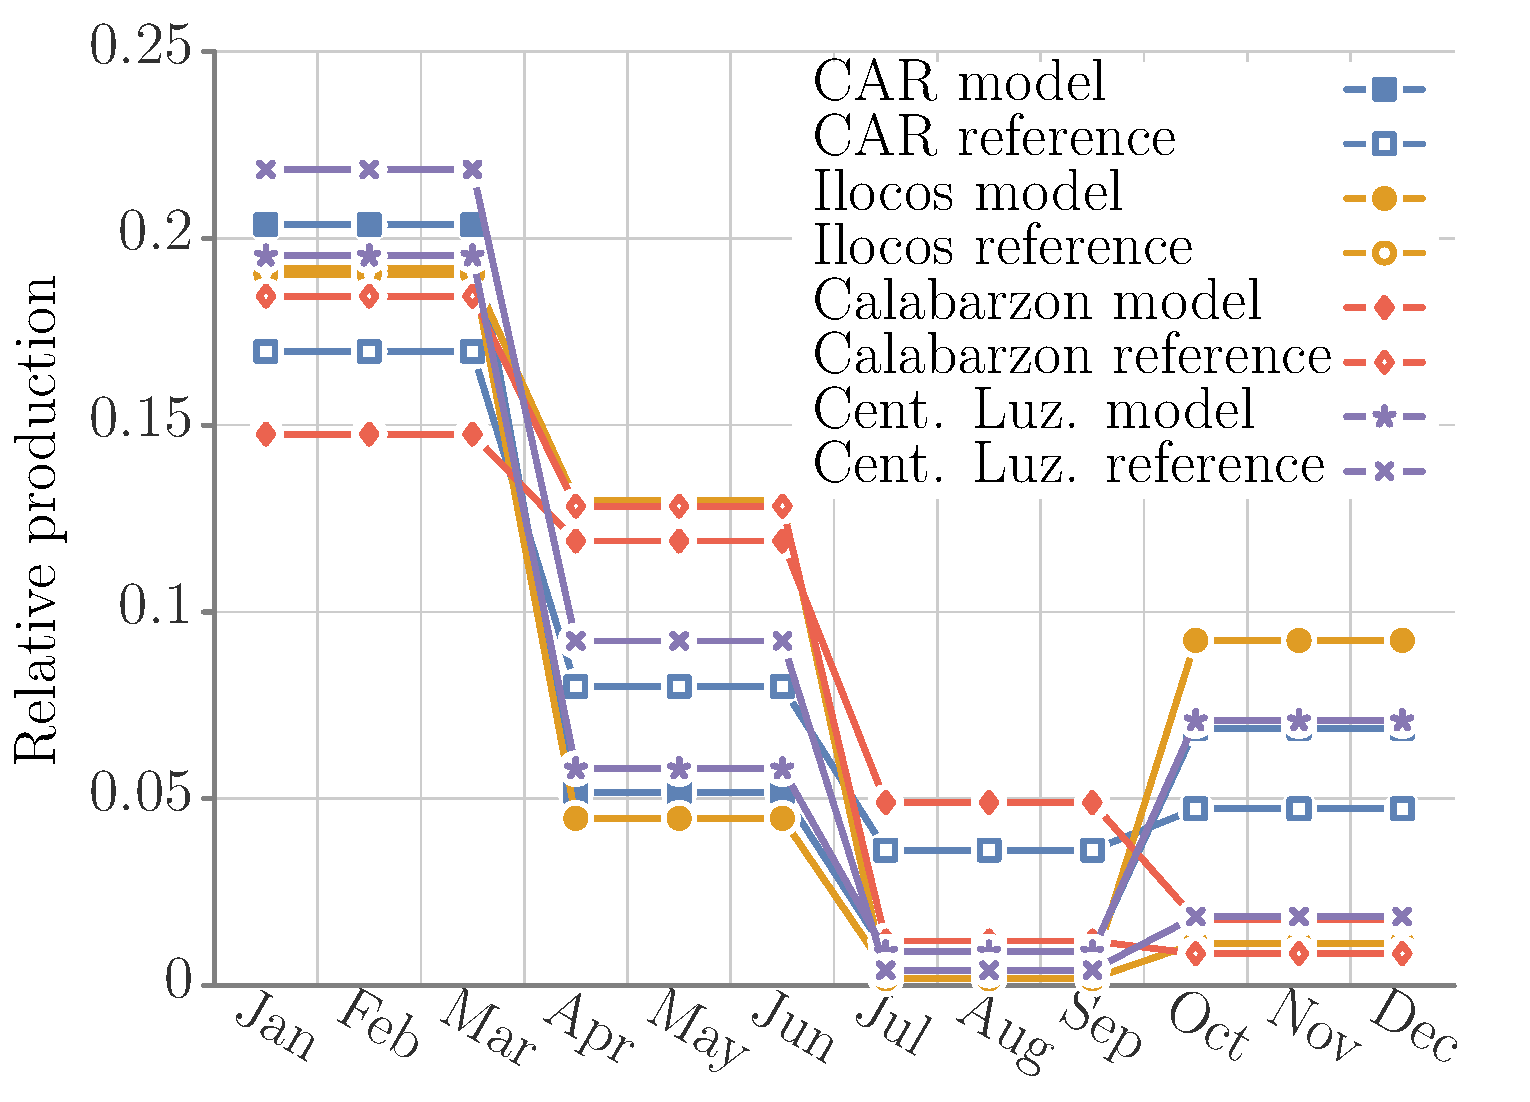
\includegraphics[width=\textwidth]{../production/results/prod_tomato_PHL_north.pdf}
\caption{Philippines tomato production compared with growing season
    information~\cite{psa2017} (North)}
\end{subfigure}
\begin{subfigure}[b]{.32\textwidth}
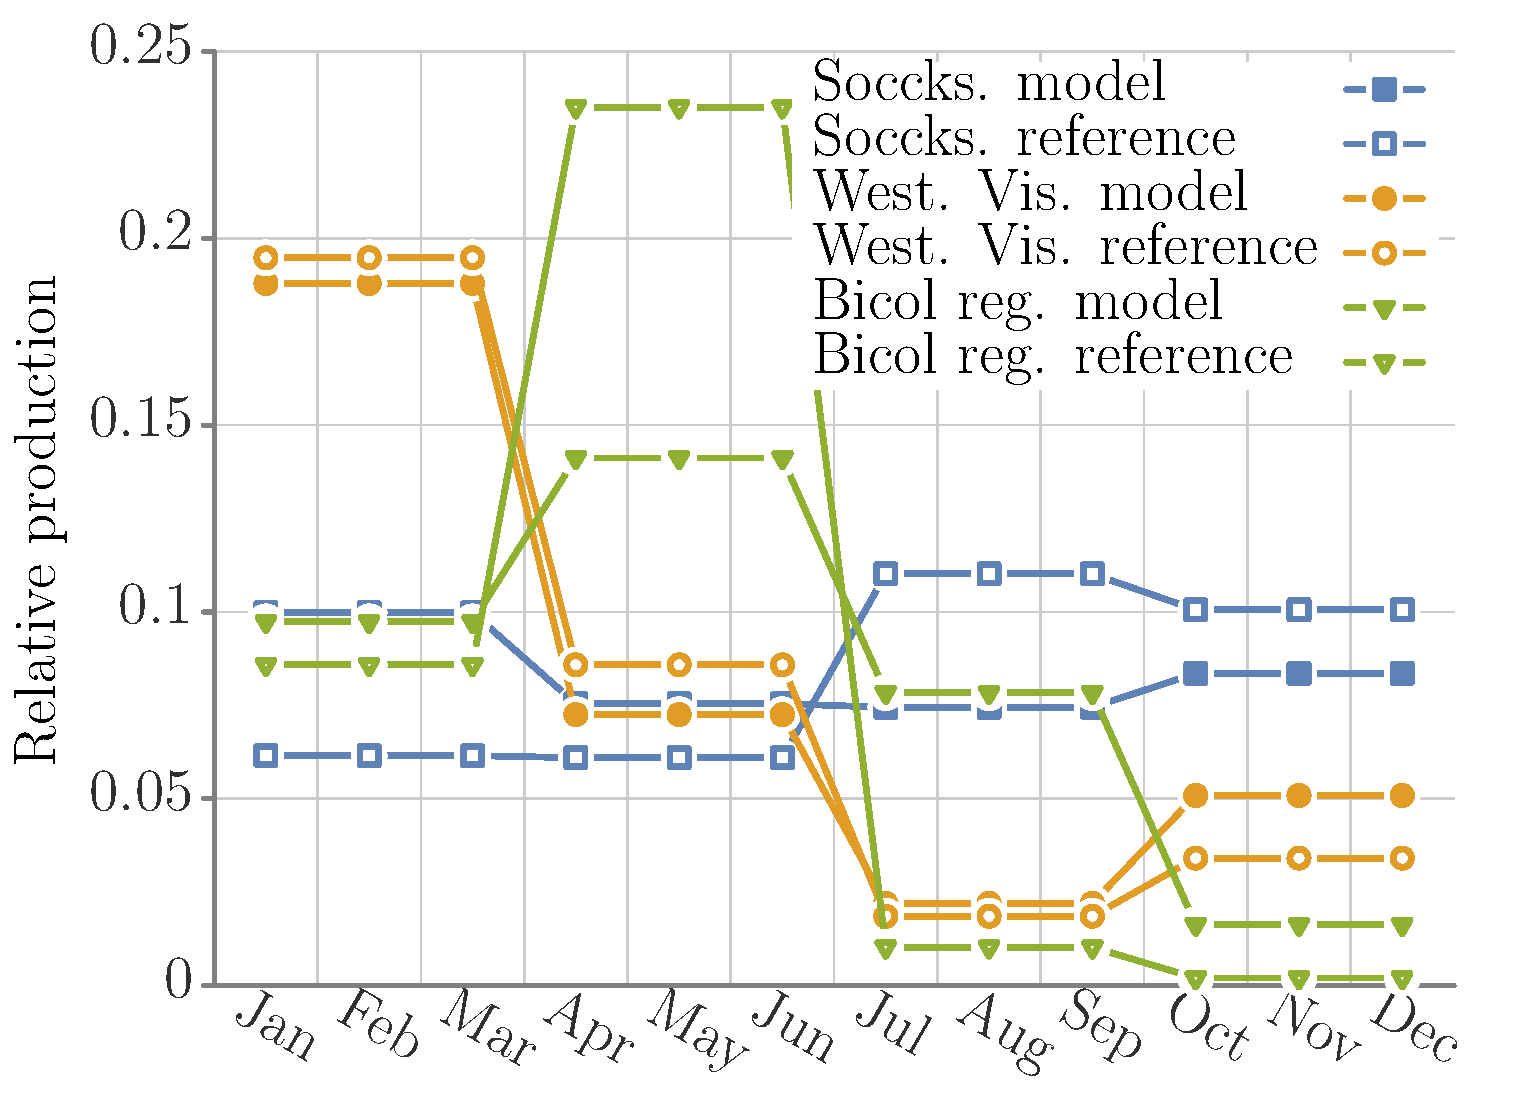
\includegraphics[width=\textwidth]{../production/results/prod_tomato_PHL_central.pdf}
\caption{Philippines tomato production compared with growing season
    information~\cite{psa2017} (Central and South)}
\end{subfigure}
\begin{subfigure}[b]{.32\textwidth}
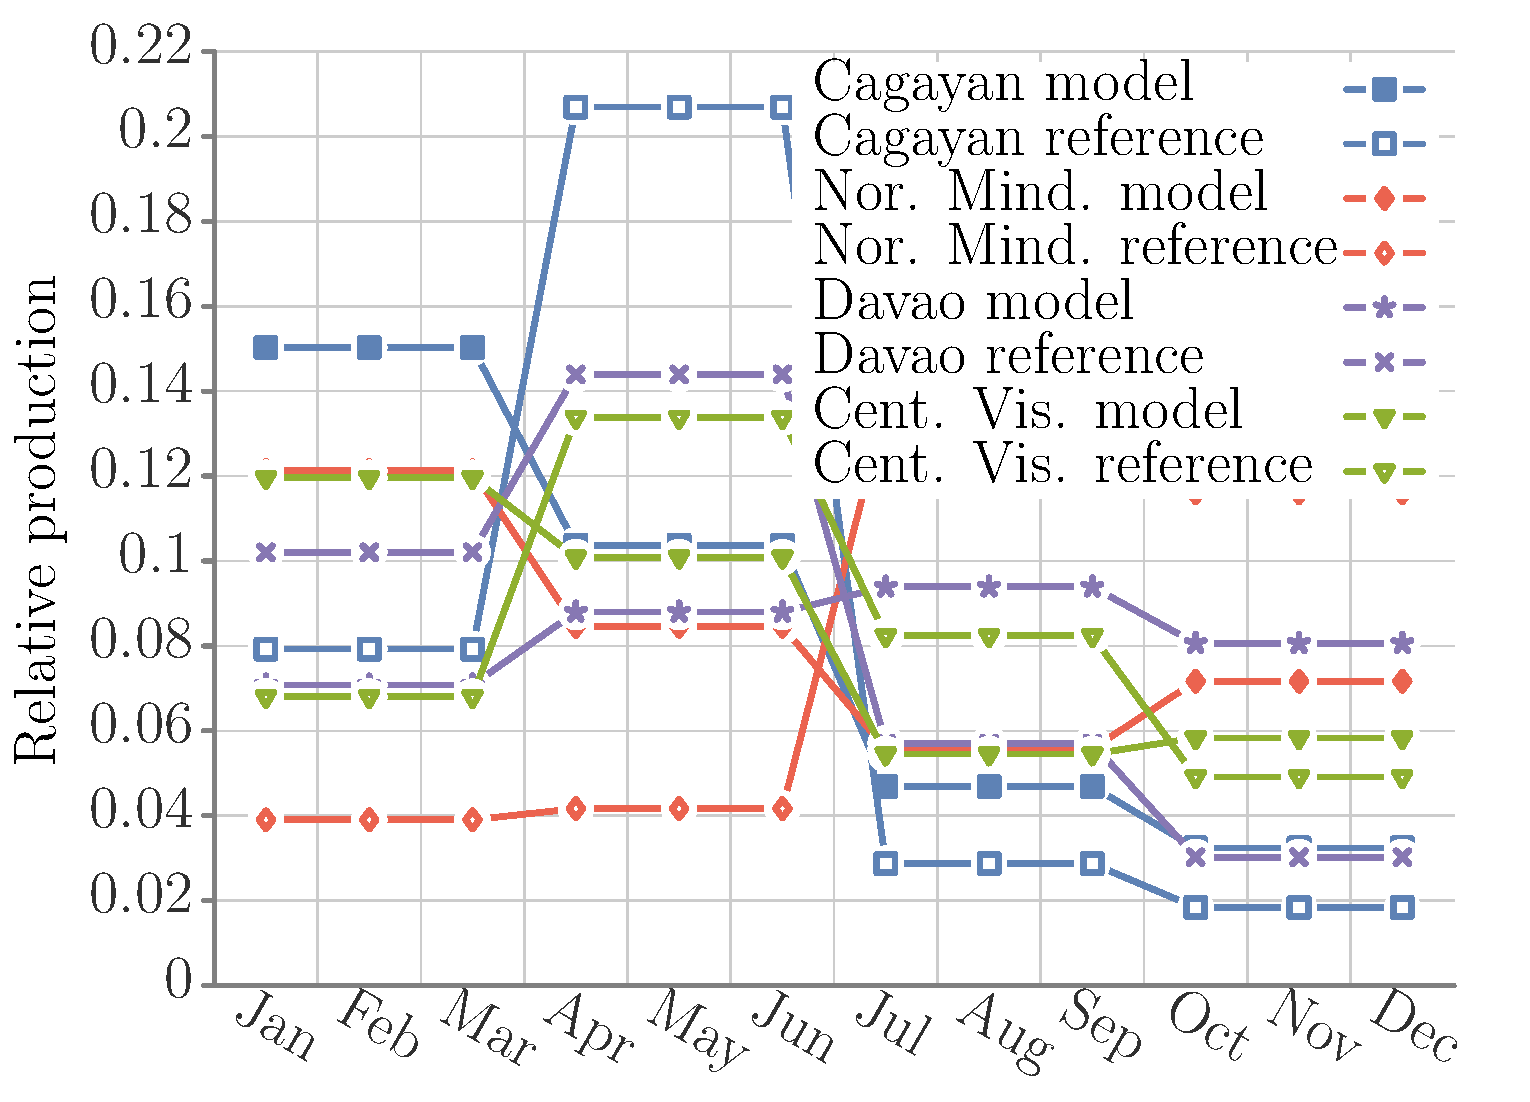
\includegraphics[width=\textwidth]{../production/results/prod_tomato_PHL_exceptions.pdf}
\caption{Philippines tomato production compared with growing season
    information~\cite{psa2017}: Regions with mismatch.}
\end{subfigure}
\caption{Comparing relative production as per the regression model with
quantitative/qualitative reports for different regions. For the plots
corresponding to the
regression model we chose representative cells for each administrative
region.
\label{fig:seasonalProd}}
\end{figure}
%%
%% \begin{figure}
%% \label{fig:sa}
%% \vspace{-5cm}
%% 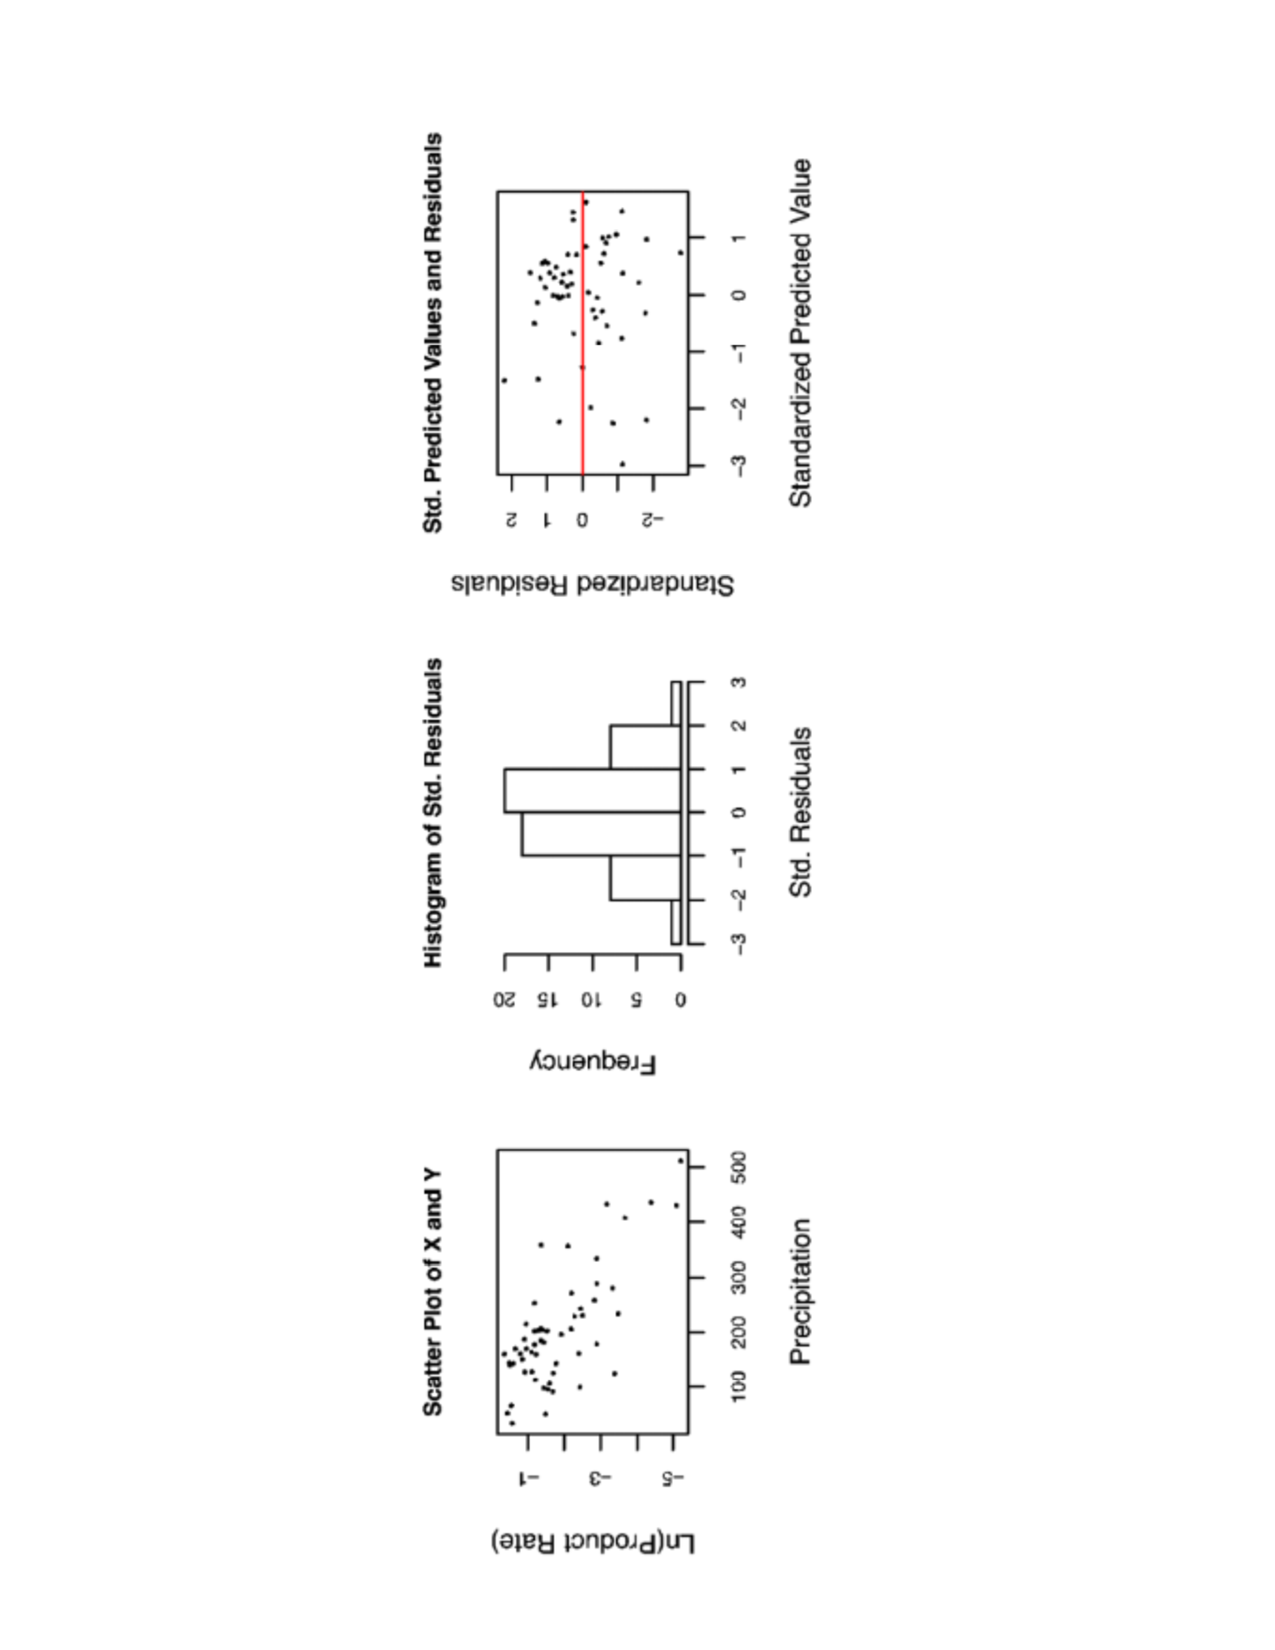
\includegraphics[width=0.8\textwidth,angle=-90,origin=c]{figs/SA_image.pdf}
%% \vspace{-7cm}
%% \caption{Validation of Linearity, Normality, and Homogeneity}
%
%\end{figure}
\subsection{Network construction}
\label{sec:netcon}
For each country, the domestic flow was estimated using a doubly
constrained gravity
model~\cite{venkatramanan2019modeling,kaluza2010complex}. For a city~$i$,
let~$O_i$ and~$I_i$ denote total outflow and total inflow respectively, and
$\locality(i)$ denotes all cells which are assigned to it.  The
flow~$F_{ij}$ from city~$i$ to city~$j$ is given by
%%
\(
   F_{ij}(t)=a_i(t)b_j(t)O_i(t)I_j(t)f(d_{ij}),
\)
%%
where, $d_{ij}$ is the time to travel from~$i$ to~$j$, and $f(\cdot)$ is
the \emph{distance deterrence function}:
$d_{ij}^{-\beta}\exp(-d_{ij}/\kappa)$, where~$\beta$ and~$\kappa$ are
tunable parameters. The coefficients~$a_i$ and~$b_j$ are computed through
an iterative process such that the total outflow and total inflow at each
node agree with the input values~\cite{kaluza2010complex}. Overall, we
have~12 networks representing flows for each month. The outflows and
inflows are calculated as follows:
%%
\begin{align}\label{eqn:flow}
    O_i(t)&=\produce(i,t)+\import(i,t)-\export(i,t)-\process(i,t),\\
    I_i(t)&=\consume(i)\,.
\end{align}
%%
Here,~$\produce(i,t)$ is the monthly production and~$\consume(i)$ is the
population of the locality as a surrogate to consumption. The latter is the
sum total of population in every cell that belong to the locality.
$\export$ and ~$\import$ are the monthly total export to and import from
outside the country respectively. $\process(i,t)$ is the tomato produced
for processing. Since for this purpose tomato is typically cultivated and
consumed locally, we subtract this volume from the outflow.
Country specific details of how locality attributes were estimated is in
Section~\ref{sec:locAttrib}.
%% We did not incorporate international trade as the volume is negligible compared to
%% domestic production with the exception of trade between Malaysia and Singapore. 
%% More details in this regard are provided in Section~\ref{S:sec:locAttrib}.

\subsection{Locality production, consumption, imports, exports and processing}
\label{sec:locAttrib}
Monthly tomato production (consumption) at a locality was obtained by
aggregating production (population) at all cells that belong to it.
Population data was obtained from Landscan (Table~\ref{tab:data}).  For
most countries, imports and exports are a small fraction of domestic
production. The main exceptions were the significant tomato imports from
India to Bangladesh and trade between Malaysia and Singapore. We identified
major routes of trade from India to Bangladesh~\cite{EIIndia2015} and the
total imports from India (FAOSTAT) was distributed uniformly between three
cities close to the border with India along these routes. Finally, these
imports were evenly distributed for the later half of the year since
Bangladesh imports mostly during the rainy season. To capture the
significant trade between Singapore and Malaysia, we included Singapore in
the domestic flow network of Malaysia as there is high interaction between
the two countries.  The resulting flow from the gravity model from Malaysia
to Singapore was obtained by aggregating network flows across months and
across edges with Singapore as destination. This flow was comparable to the
annual imports from Malaysia to Singapore. With the exception for
Thailand~\cite{mict2013}, Vietnam~\cite{wijk2007} and Cambodia (pers.
comm.), there is no information on the amount of tomato production consumed
by the processing industry even though there is evidence of processing
industry in Malaysia and Indonesia. For each locality in Thailand, we
scaled the monthly production by the ratio annual production of fresh
tomatoes over total annual production (fresh and processed).

For consumption, we used country-level
production~\cite{faostatConsumption}, which was available for half of the
countries. For Singapore, we estimated it as the difference between total
inflow (production and imports) and total outflow (exports) based on FAO
data. For Vietnam, Wijk~et~al.~\cite{wijk2007} provides this information.
For Myanmar, Cambodia and Laos, we found no information. We used median
consumption for the region. We also analysed consumption with respect to
per capita gross domestic product (GDP). However, we did not find any
correlation between GDP and consumption both globally as well as restricted
to the study region. In
Venkatramanan~et~al.~\cite{venkatramanan2019modeling}, consumption was
modelled as a function of population and Gross Domestic Product (GDP). In
the study region, analysing FAO data on
consumption~\cite{faostatConsumption} we did not find any relation between
GDP and consumption.

\subsection{Validation of domestic trade flows}
\label{sec:tradeFlows}
Since no market-to-market flow data is available for the region, we
searched the literature for evidence of tomato trade between cities or
regions for each country. Even this information is hardly
available. The next step was to further generalise the search by
considering the flow of vegetables. The results of our comparison of the
networks obtained using gravity flow model with literature are shown
Figure~\ref{fig:trade_flows}. Our general observations
as follows: (i)~To obtain good representation of trade flow, at minimum,
region/state level data of production is required; and (ii)~densely populated
urban pockets are a good representation of consumption centres. Some country
specific details follow.
%%
\begin{figure}[!ht]
\centering
\subcaptionbox{Bangladesh\label{fig:bgdFlow}}
{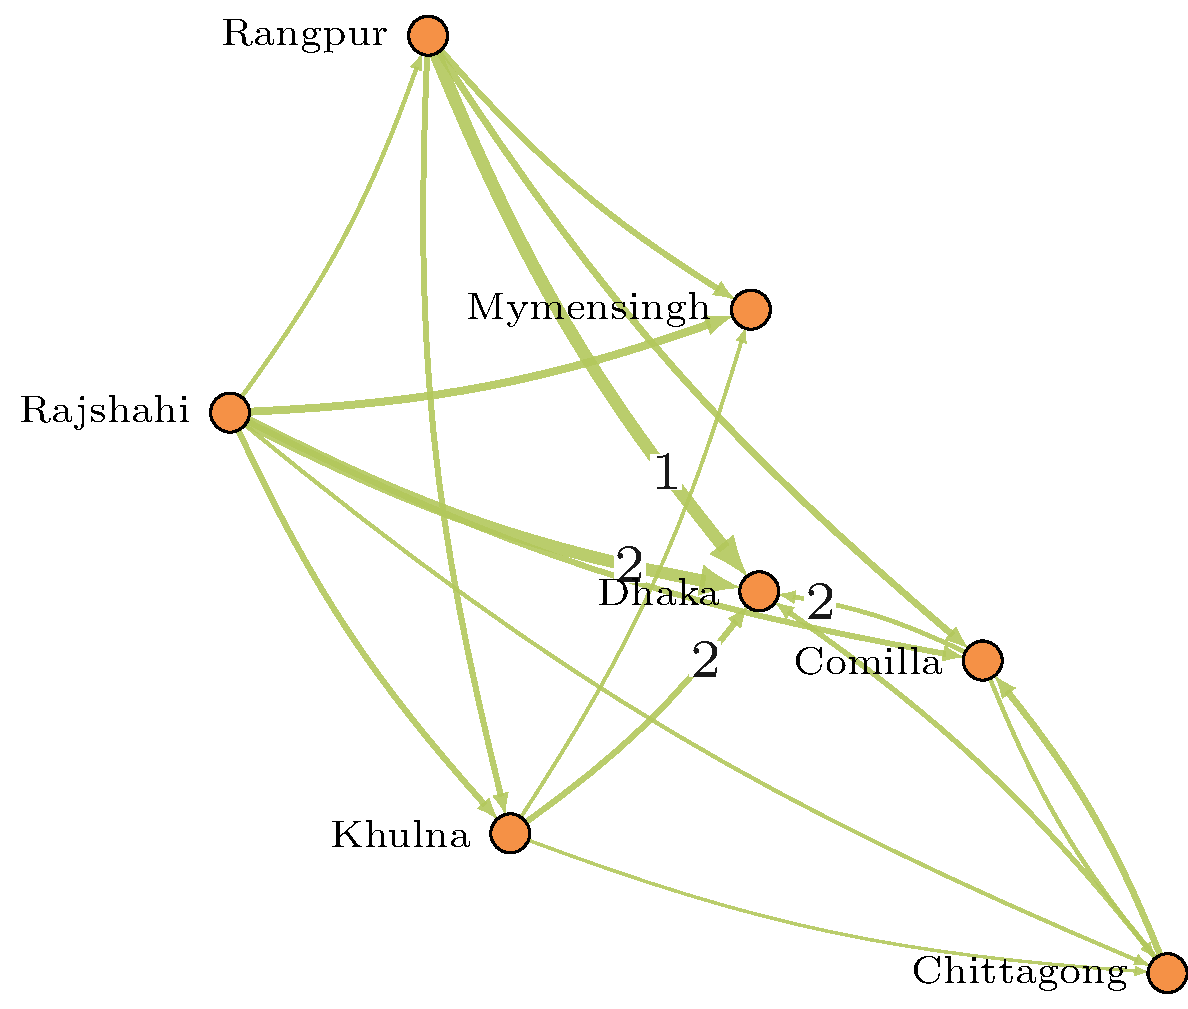
\includegraphics[width=.33\textwidth]{../long_distance/results/validation/BGD_flows_precip1_b2_k500.pdf}}
%%
\subcaptionbox{Myanmar\label{fig:mmrFlow}}
{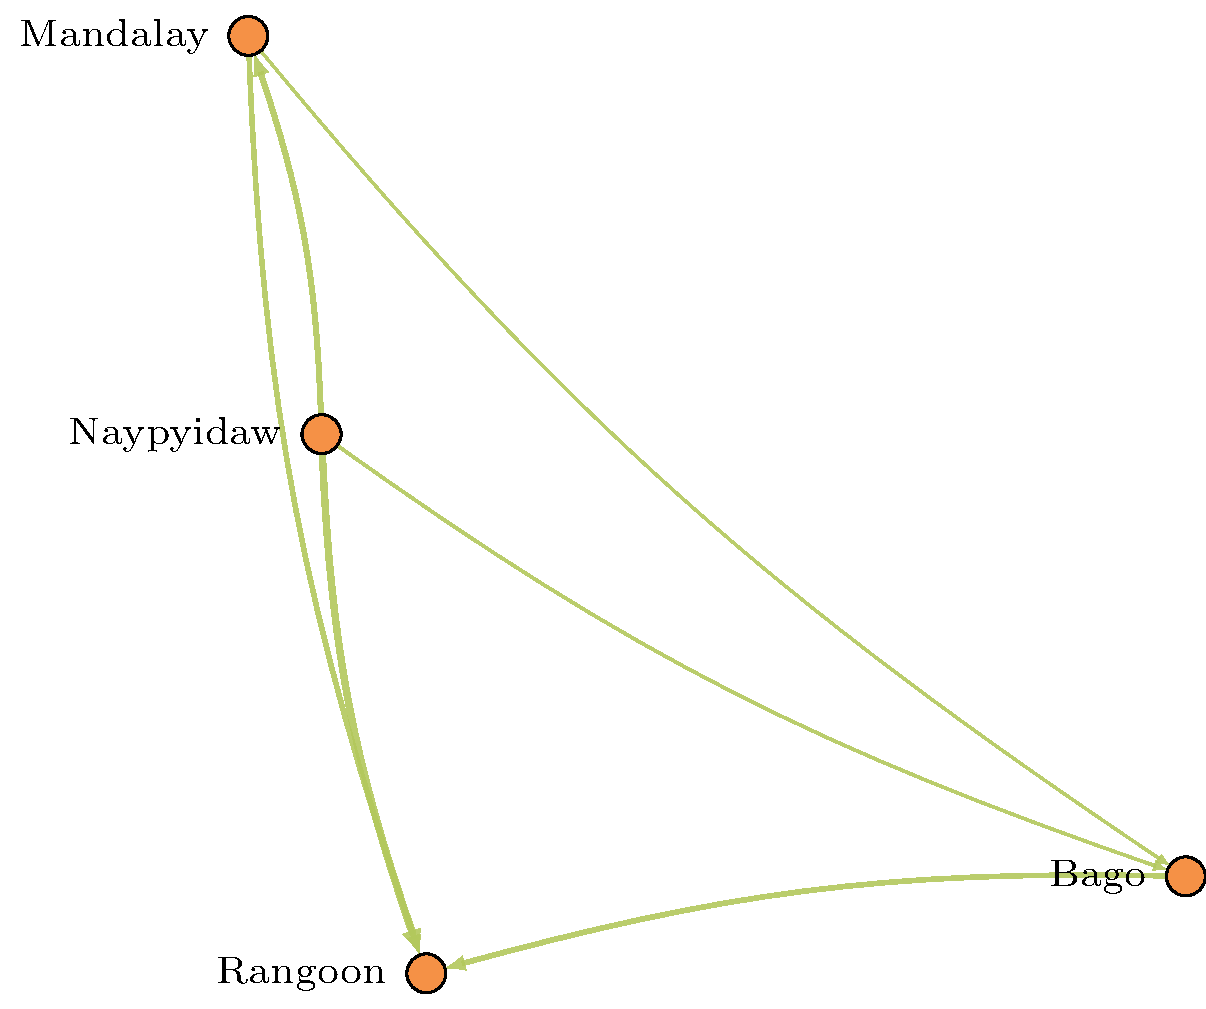
\includegraphics[width=.33\textwidth]{../long_distance/results/validation/MMR_flows_precip1_b2_k500.pdf}}
%%
\subcaptionbox{Thailand\label{fig:thaFlow}}
{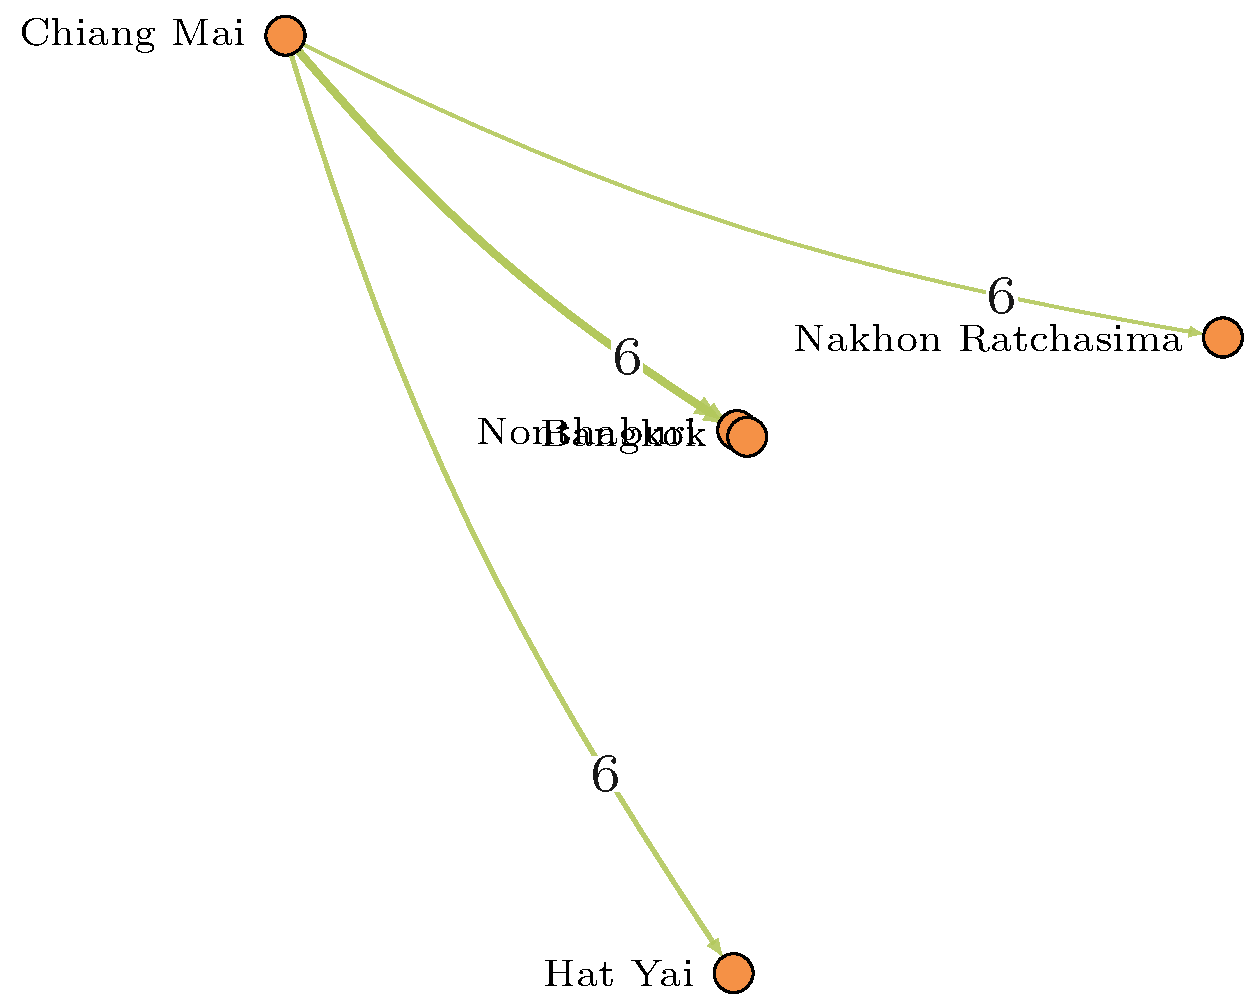
\includegraphics[width=.33\textwidth]{../long_distance/results/validation/THA_flows_precip1_b2_k500.pdf}}
%%
\subcaptionbox{Vietnam\label{fig:vnmFlow}}
{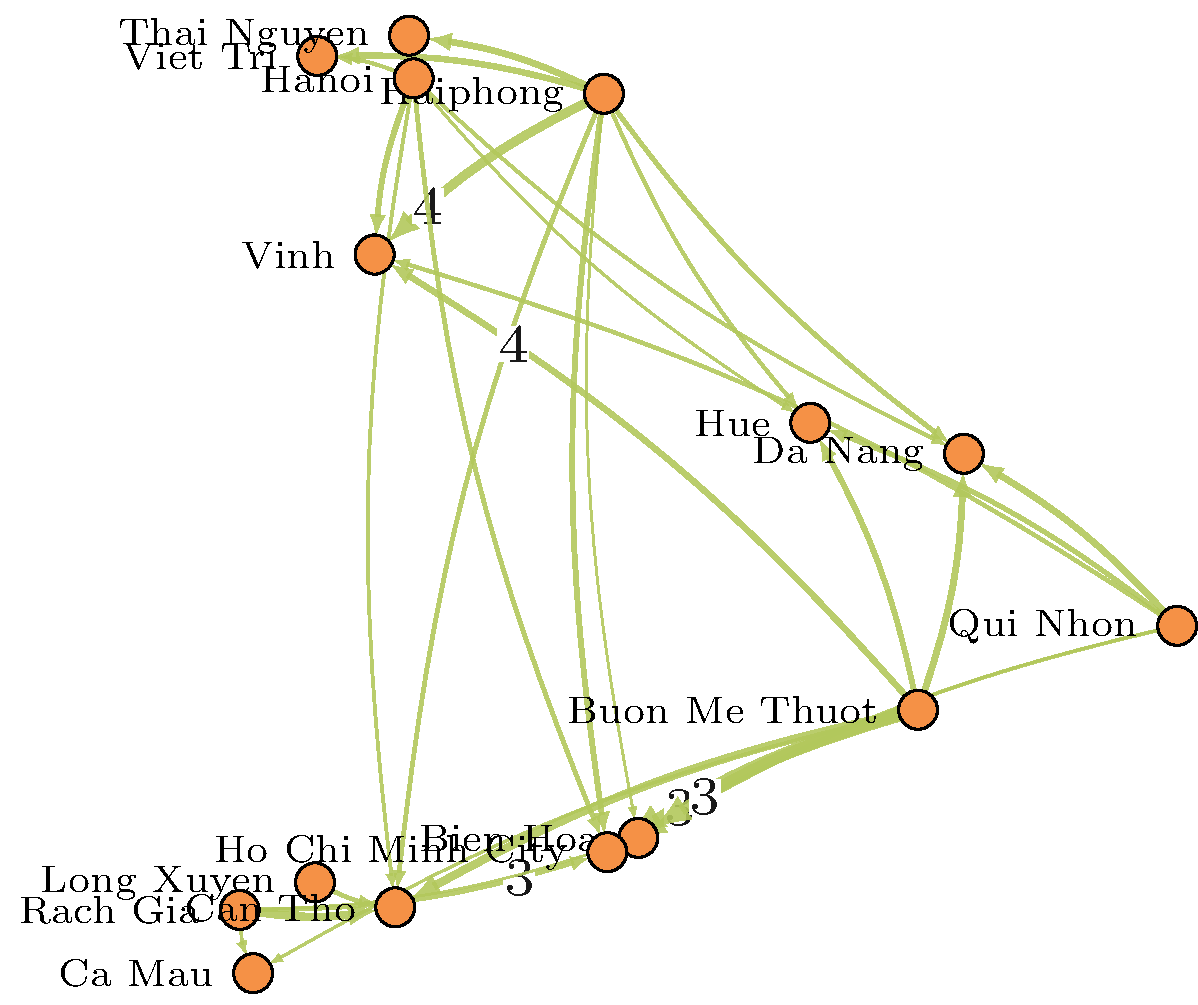
\includegraphics[width=.33\textwidth]{../long_distance/results/validation/VNM_flows_precip1_b2_k500.pdf}}
%%
\subcaptionbox{Malaysia and Singapore\label{fig:mysFlow}}
{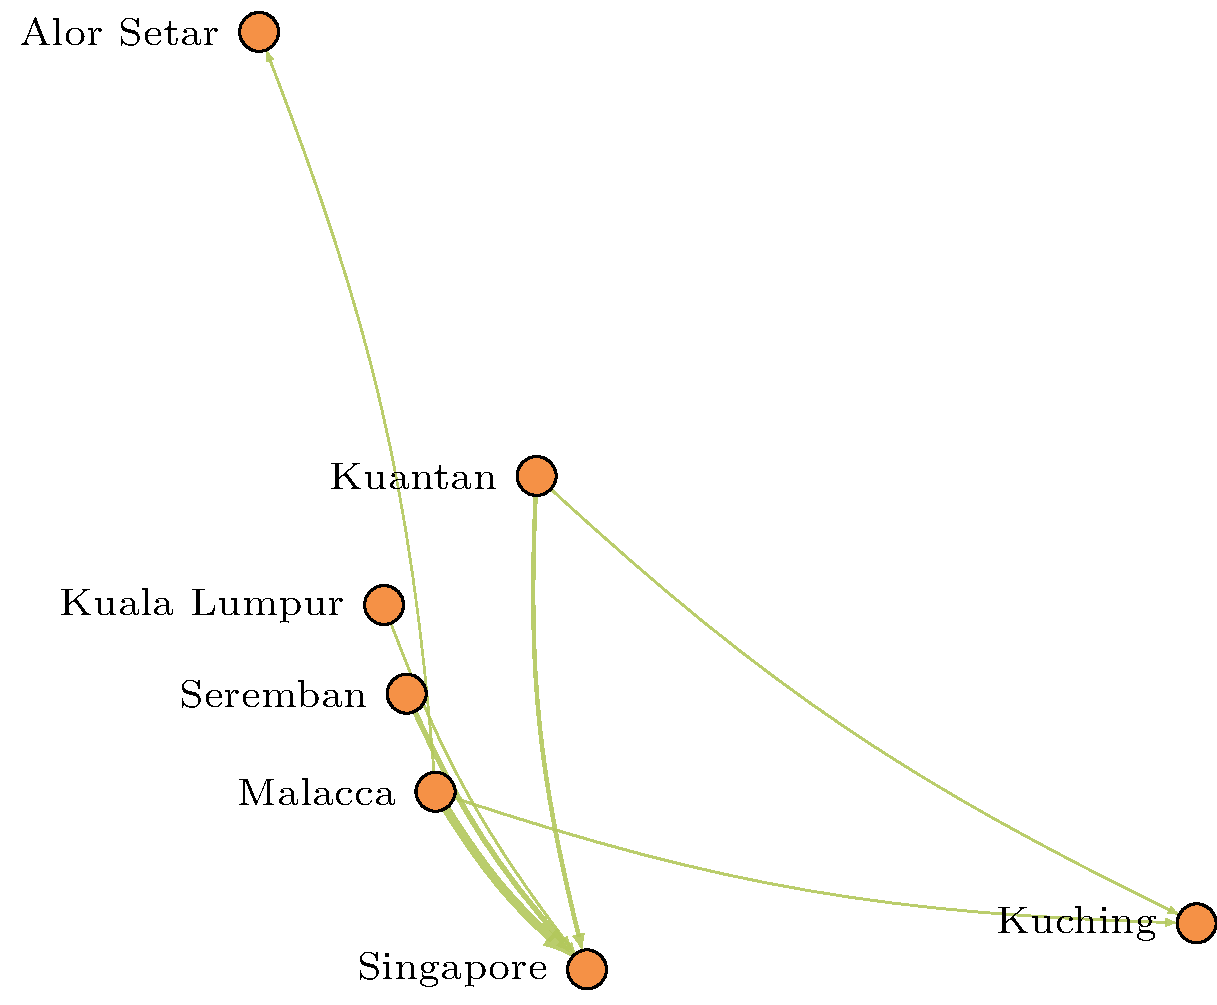
\includegraphics[width=.33\textwidth]{../long_distance/results/validation/MYS_flows_precip1_b2_k500.pdf}}
%%
\subcaptionbox{Indonesia\label{fig:idnFlow}}
{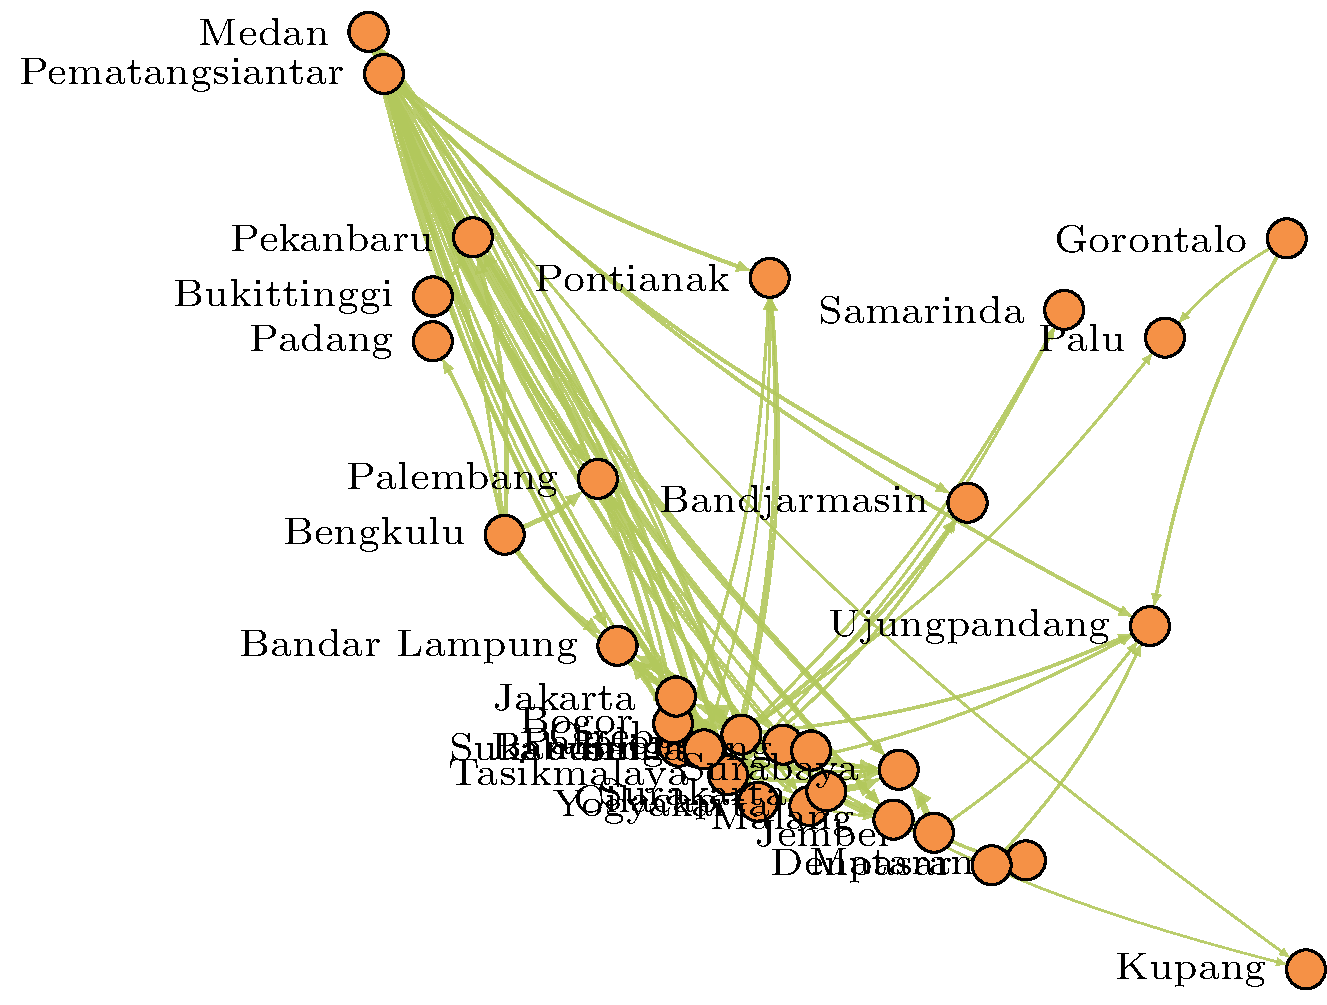
\includegraphics[width=.33\textwidth]{../long_distance/results/validation/IDN_flows_precip1_b2_k500.pdf}}
%%
\subcaptionbox{Philippines\label{fig:phlFlow}}
{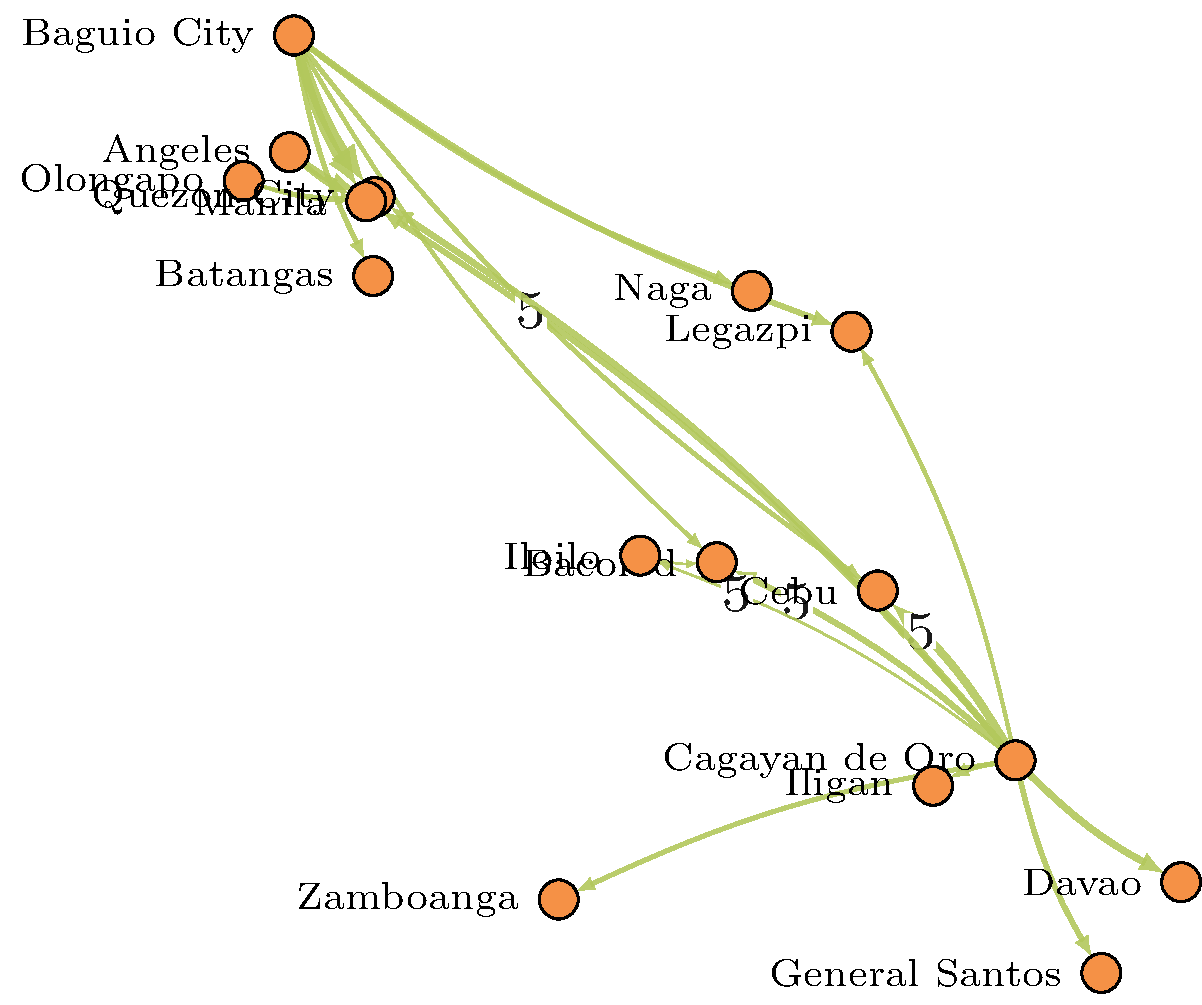
\includegraphics[width=.33\textwidth]{../long_distance/results/validation/PHL_flows_precip1_b2_k500.pdf}}
%%
\subcaptionbox{References corresponding to trade flow
evidence.}[.5\textwidth]{
    \small
\begin{tabular}{cl}
\hline
Index & Citation \\\hline
1 & Daily Sun 2018 \cite{dailysun2018}\\
2 & Karim et al. 2016 \cite{karim2016}\\
3 & Cadilhon et al. 2006 \cite{cadilhon2006}\\
4 & Wijk et al. 2007 \cite{wijk2007}\\
5 & Ledesma 2011 \cite{ledesma2011}\\
6 & Johnson et al. 2008 \cite{johnson2008}\\\hline
\end{tabular}
}
\caption{\textbf{Long-distance annual trade flows resulting from the gravity model.}
We combined monthly flows and to avoid clutter, we have displayed only major
    flows ($>500$). Some of the edges
    are labelled based on information from literature. The references
    corresponding to the labels are listed in (h). For Laos, Cambodia and
    Brunei, there are no flows as there is only one locality in each
    country. \label{fig:trade_flows}}
\end{figure}
%%
\paragraph{Bangladesh.}
There is evidence of vegetable flow from Rangpur region to Dhaka
particularly during winter~\cite{dailysun2018,independent2018}. The flow
from Southwest Bangladesh to Dhaka~\cite{karim2016} is captured by the edge
from Khulna to Dhaka (Figure~\ref{fig:bgdFlow}). We assigned import of
tomato from India to cities in the border based on information on important
trade routes~\cite{EIIndia2015}.  Since, there is no data on volume, we
distributed it evenly.
%%
\paragraph{Vietnam.}
There are primarily two consumption centres: Ho Chi Minh City in the south
supplied by Central Highlands and the Mekong River Delta, and
Hanoi-Haiphong urban centres in the north supplied by Red River Delta. For
Ho Chi Minh City, Lam Dong is the main district that supplies
vegetables~\cite{cadilhon2006}.  In our model (Figure~\ref{fig:vnmFlow}),
this flow is represented by Buon Me Thuot--a city in Central Highlands--to
Ho Chi Minh City. Buon Me Thuot is less than 100km away from the Lam Dong
province thus covering the production in the area. In the north, much of
the production surplus is assigned to the Haiphong locality, and therefore,
it acts as a big source for almost all localities in the north. Our network
also has some long distance edges from north to south. This is mostly due
to the large population in the south. There is not much evidence of this
flow and it could be a result of not accounting for heterogeneity in
consumption.
%%
\paragraph{Malaysia and Singapore.} We combined the locality corresponding
to Singapore with Malaysia, so that the flow between these two countries is
treated as a domestic flow as there is free movement of people and goods
between these countries. The gravity model flows from Malaysia to Singapore
is between 50,000--60,000 tonnes compared to $\approx30,000$ tonnes
according to FAOSTAT. However, our network does not capture the flow from
Cameron Highlands, major tomato producer to cities of Malaysia. This
shortcoming is mainly due to unavailability of state/province level tomato
production information.
%%
\paragraph{Philippines.} The major production centres are in Cagayan de Oro
and regions north of Manila. These are captured by our network
(Figure~\ref{fig:phlFlow}).

\subsection{Transmission probability}\label{trans}
At any given time~$t$, for a cell~$v$ and its neighbour~$v'$ corresponding
to the considered pathway, let $\infest(v',t)$ be the strength of
infestation at~$v'$. Let,~$\alpha$ be the transmission rate corresponding
to the pathway. Then, the probability that the pest will be introduced
to~$v$ from~$v'$ is given by~$1-\exp\big(-\alpha\infest(v',t)\big)$. The
function form is similar to that in~\cite{newman2002spread,meyers2007}, but with
contact time between two nodes replaced with strength of infestation. Also,~$\alpha$ can be interpreted as the transmission probability
per unit infestation. Since in our case production in the cell is used as a
surrogate for~$\infest(v',t)$, it can be interpreted as the
probability of infection per unit production. \\

This form of the infection probability function has been seen before in
epidemiological models
\cite{diekmann2000mathematical,hethcote1989periodicity,hethcote1994thousand},
both continuous and discrete time models. Diekmann~et~al.
\cite{diekmann2000mathematical} 
consider a continuous time SI model, and define the probability that an
individual will not be infected with a function which relates to the form
above, taking the exponent as an integral of the "force of infection". 
%% In \cite{cantor2003sas}, we see more complexity, but we also see some
%% derivation of this function form from the "proportional hazards model".
%% They similarly consider a continuous time model and an exponential
%% probability function of remaining susceptible.
In \cite{hethcote1994thousand}, we see a discrete time version of this
function form, with the probability of still being exposed after $t$ time
steps as: $P(t) = e^{-\epsilon t}$, where $\epsilon$ relates to the
"transfer rate". This function form was derived when considering
traditional SIR models mathematically in \cite{hethcote1989periodicity}.

\section{Parameterization and simulation}
\label{sec:cart}
For each parameter setting, we evaluated the model output by comparing it
with historical invasion data from Bangladesh using a similarity score
as defined in the main document (equation~(\ref{M:eqn:similarity})). Simulations
were run with 100 repetitions. From the output we computed the empirical
probability that a cell is in state~$I$ at time~$t$, which in turn was used
to compute similarity scores.  We applied Classification and Regression
Trees~(CART) to guide parameter space exploration. Initially, the parameter
space was coarsely sampled. The parameter values are listed in
Table~\ref{M:tab:param} in the main document. For each of these samples, simulations were run
and the similarity scores computed. With the model parameters as independent
variables and similarity score as the dependent variable, we analysed the results
using CART (see Figure~\ref{fig:cart}). We chose parameter subspaces with
high similarity score (5.5 or more) and rejected those with lower values.  For
each chosen parameter subspace, the process was repeated.
%%
\begin{figure}[!ht]
    \begin{subfigure}[b]{.45\textwidth}
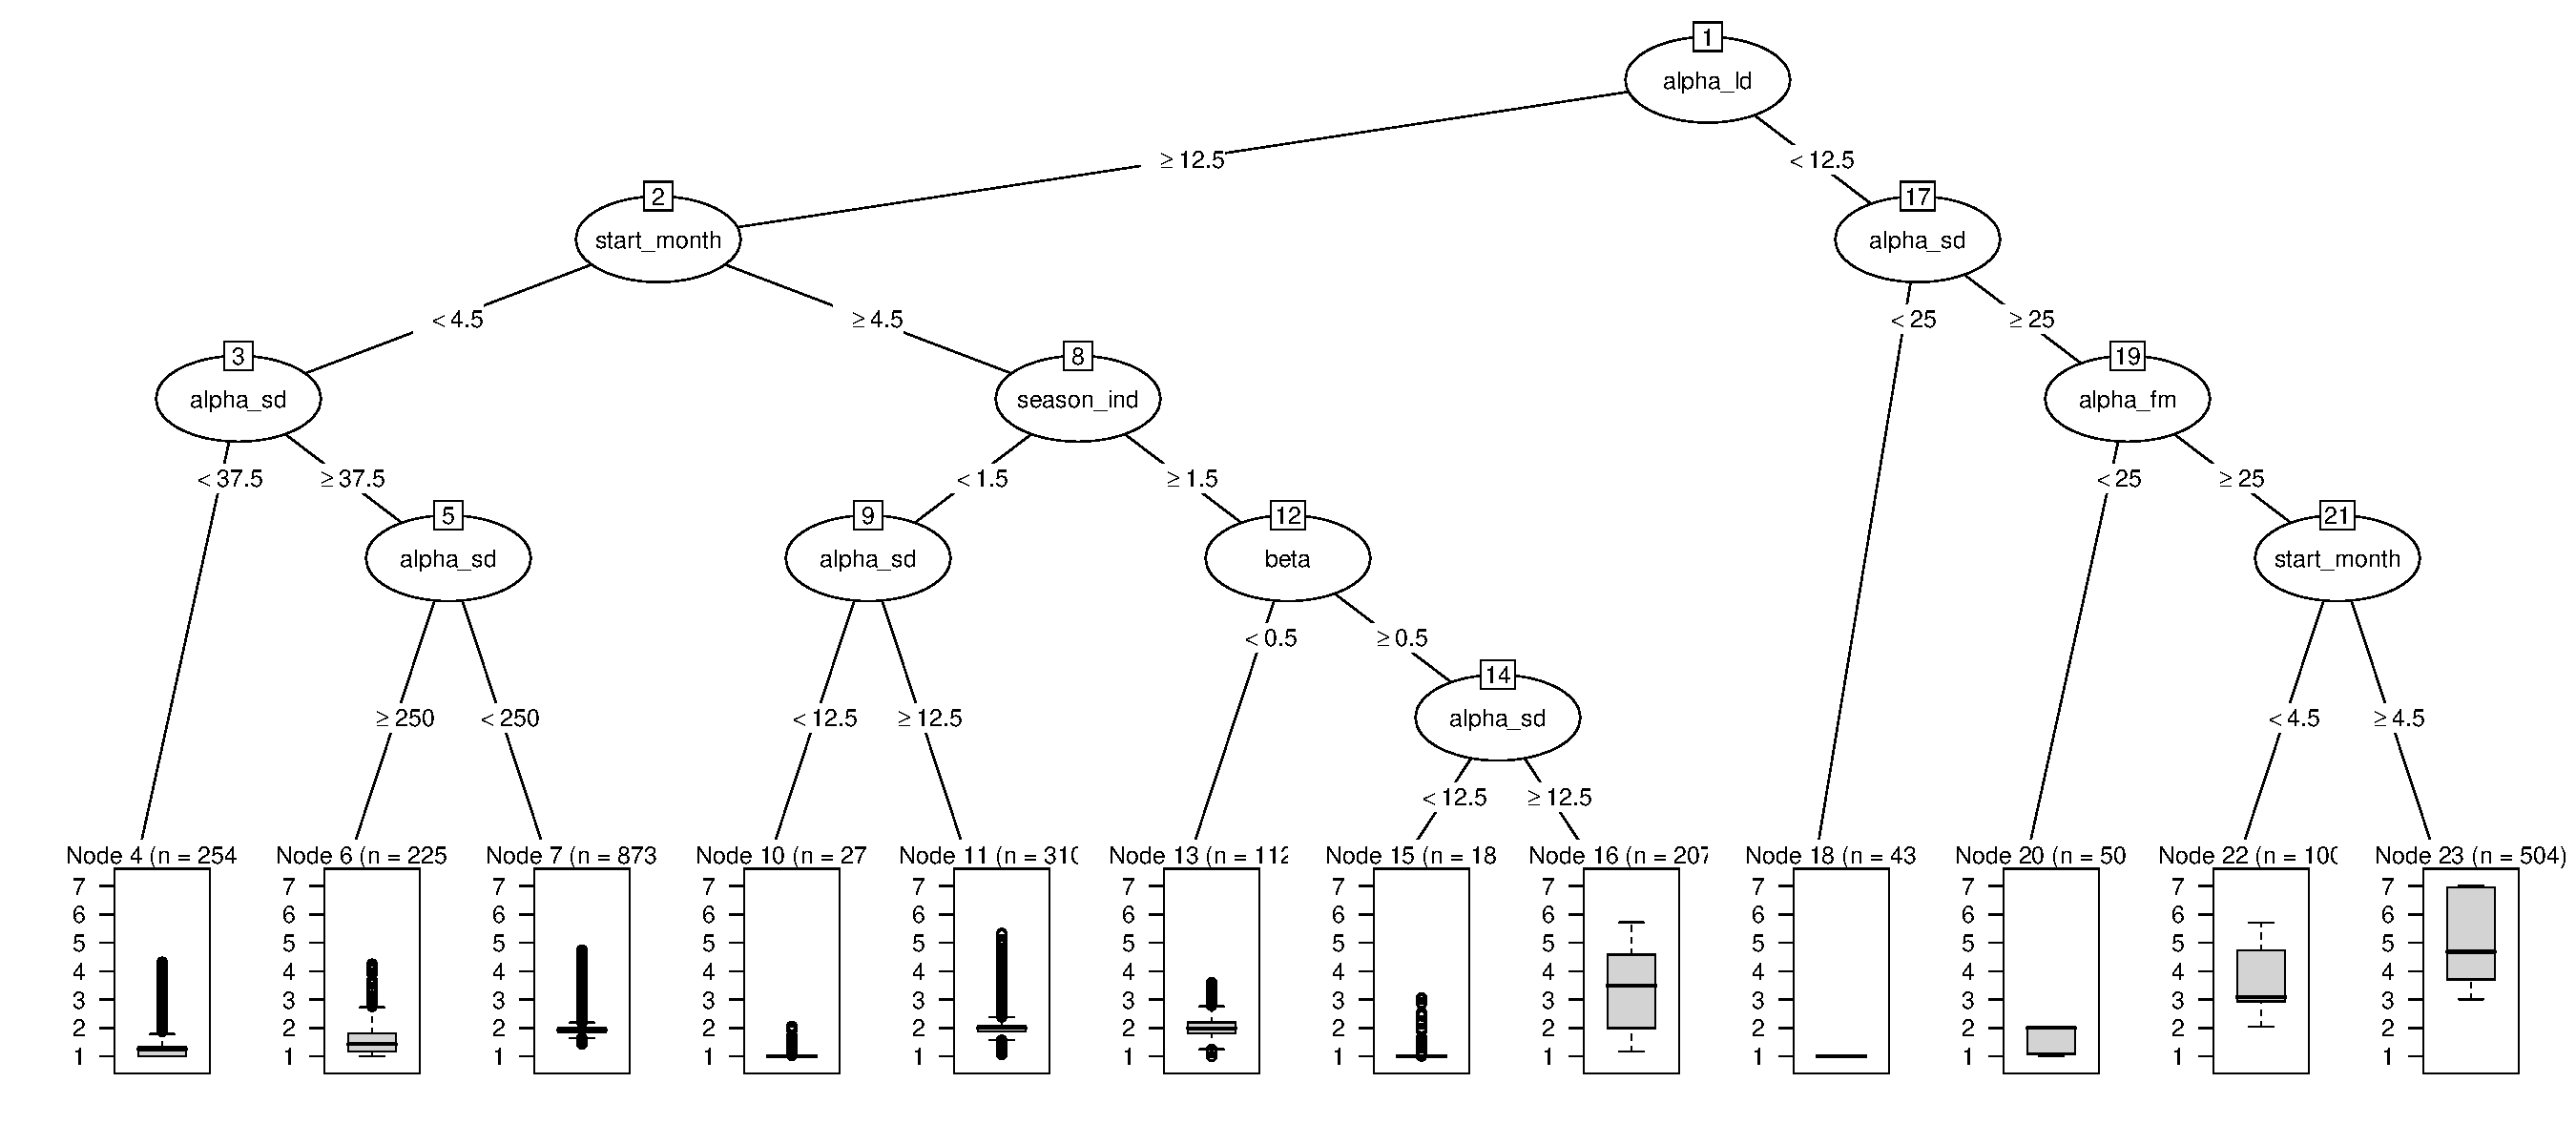
\includegraphics[width=\textwidth,trim={1cm 1cm 1cm 0cm},clip]{../cellular_automata/results/cart/m1_l1_tree.pdf}
\caption{$\mooreRange=1$, $\ell=1$}
    \end{subfigure}
    \begin{subfigure}[b]{.45\textwidth}
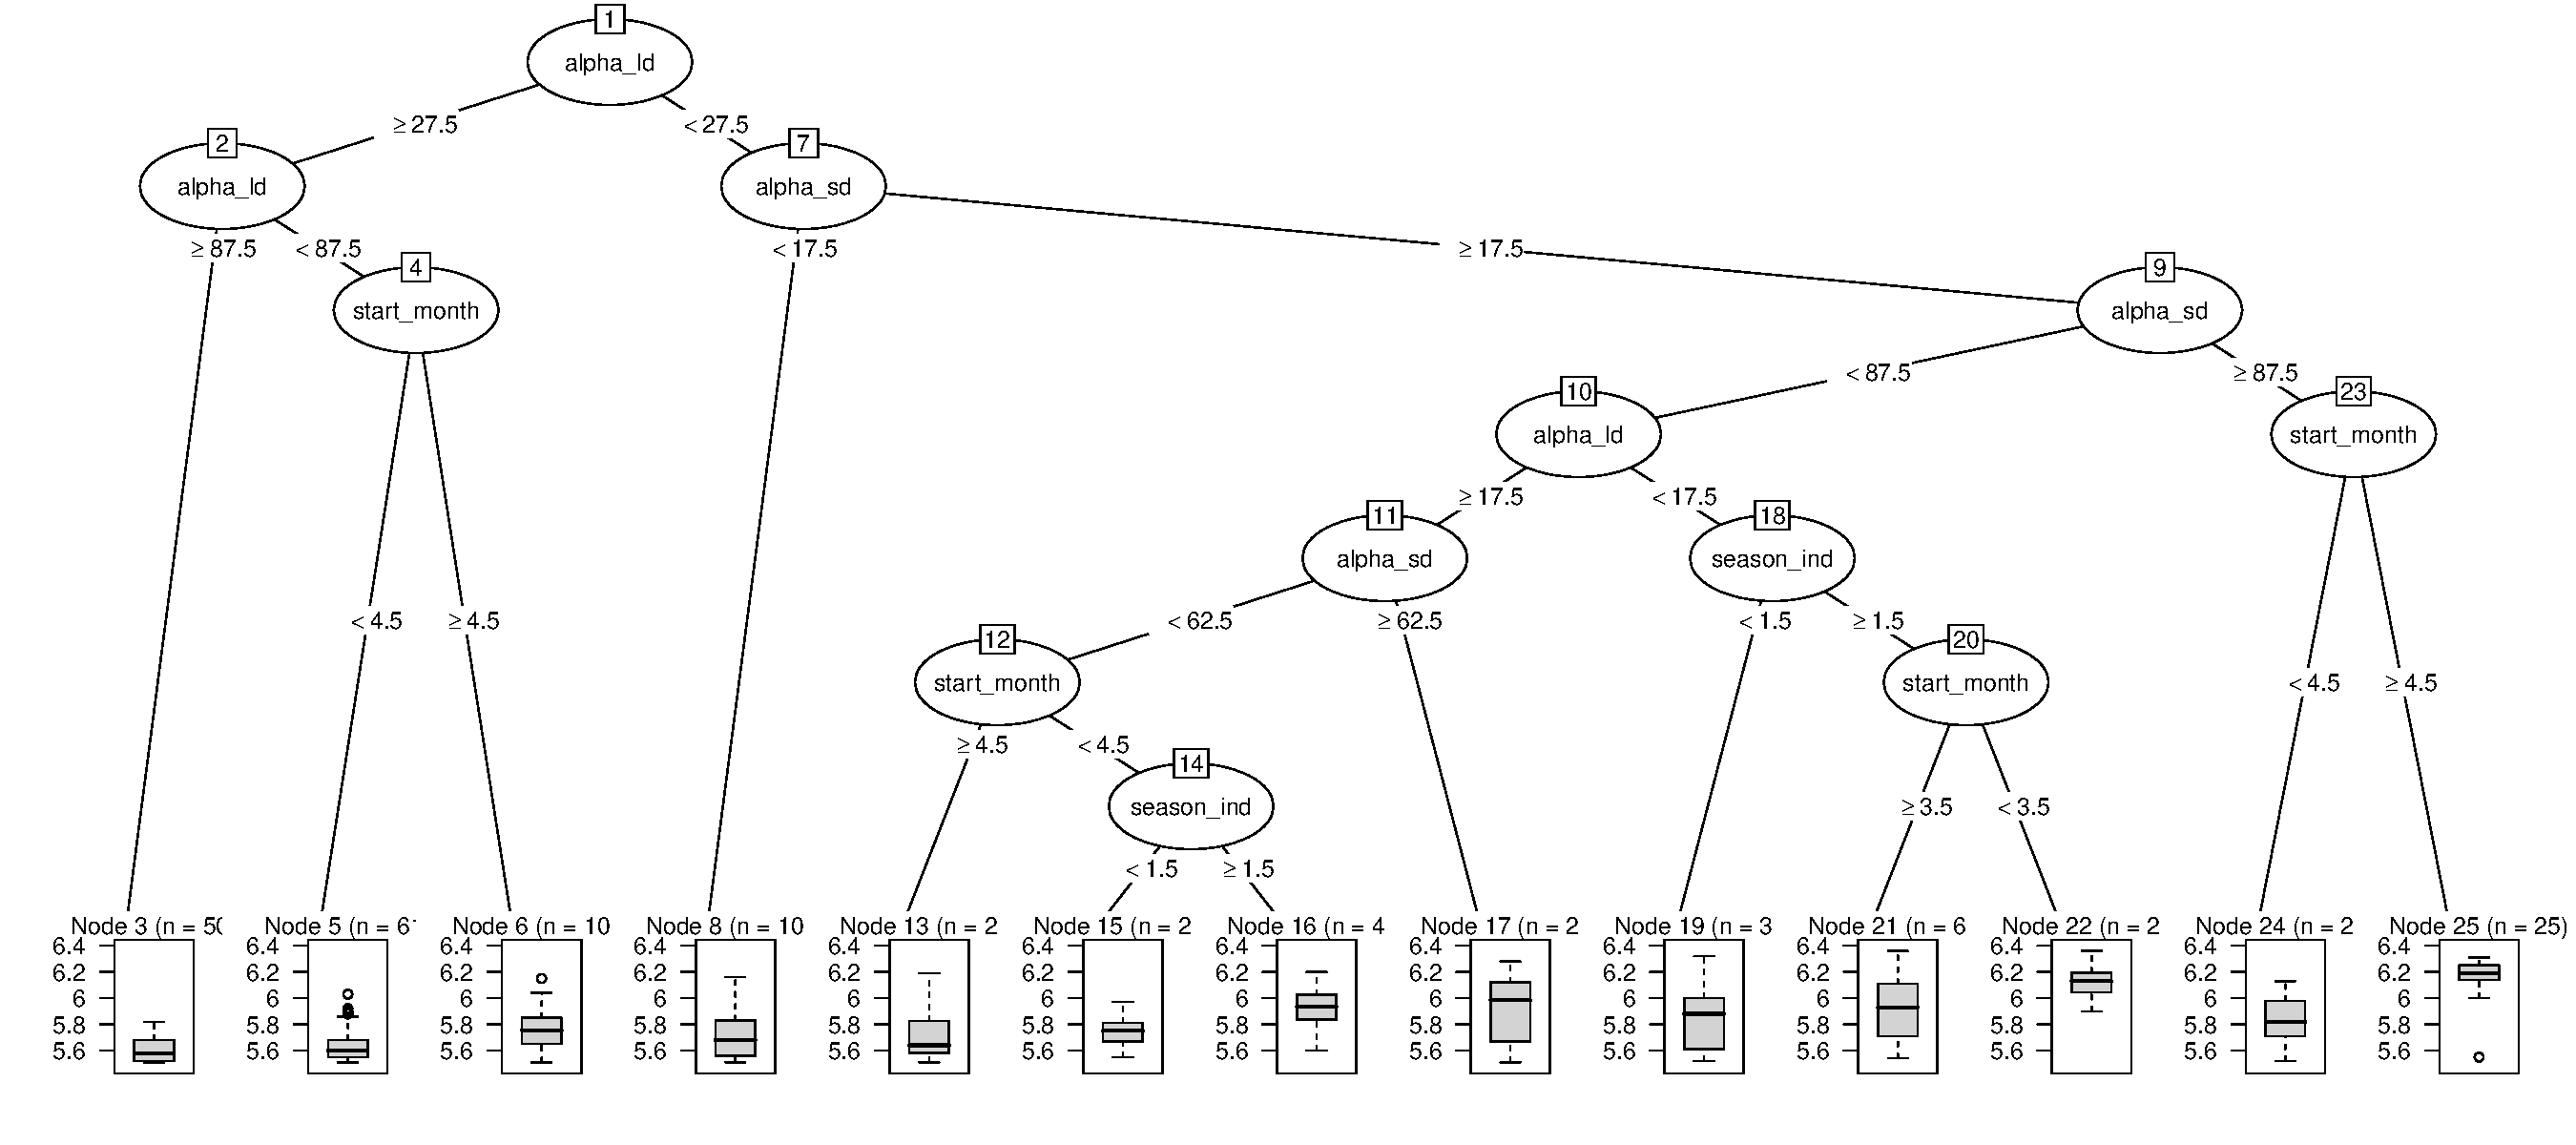
\includegraphics[width=\textwidth,trim={1cm 1cm 1cm 0cm},clip]{../cellular_automata/results/cart/m1_l2_tree.pdf}
\caption{$\mooreRange=1$, $\ell=2$}
    \end{subfigure}
    \begin{subfigure}[b]{.45\textwidth}
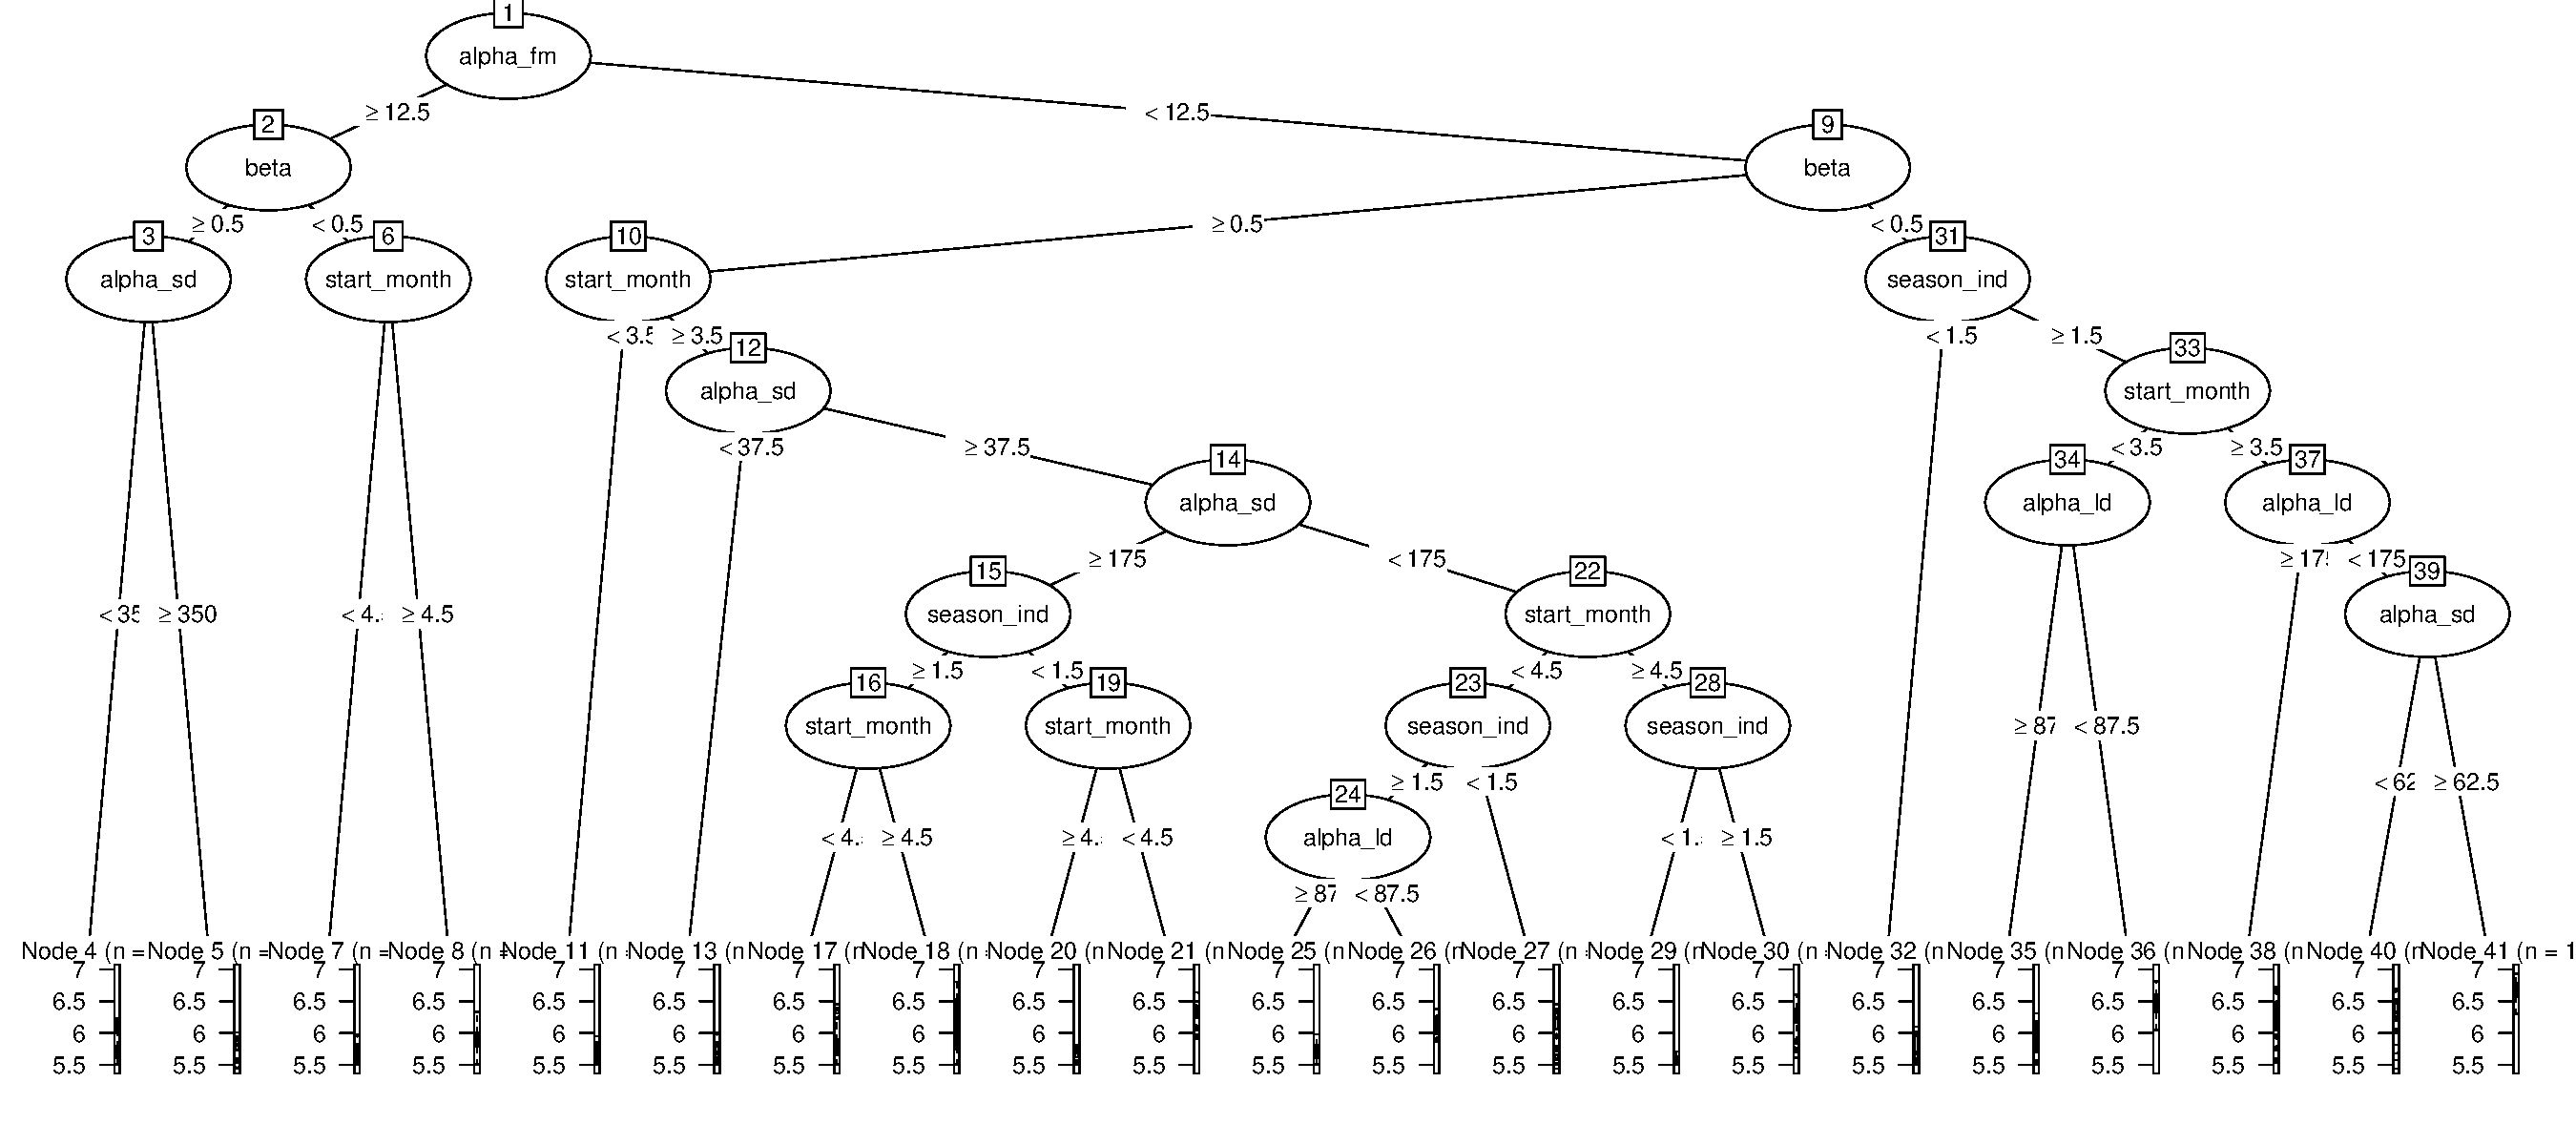
\includegraphics[width=\textwidth,trim={1cm 1cm 1cm 0cm},clip]{../cellular_automata/results/cart/m1_l3_tree.pdf}
\caption{$\mooreRange=1$, $\ell=3$}
    \end{subfigure}
    \begin{subfigure}[b]{.45\textwidth}
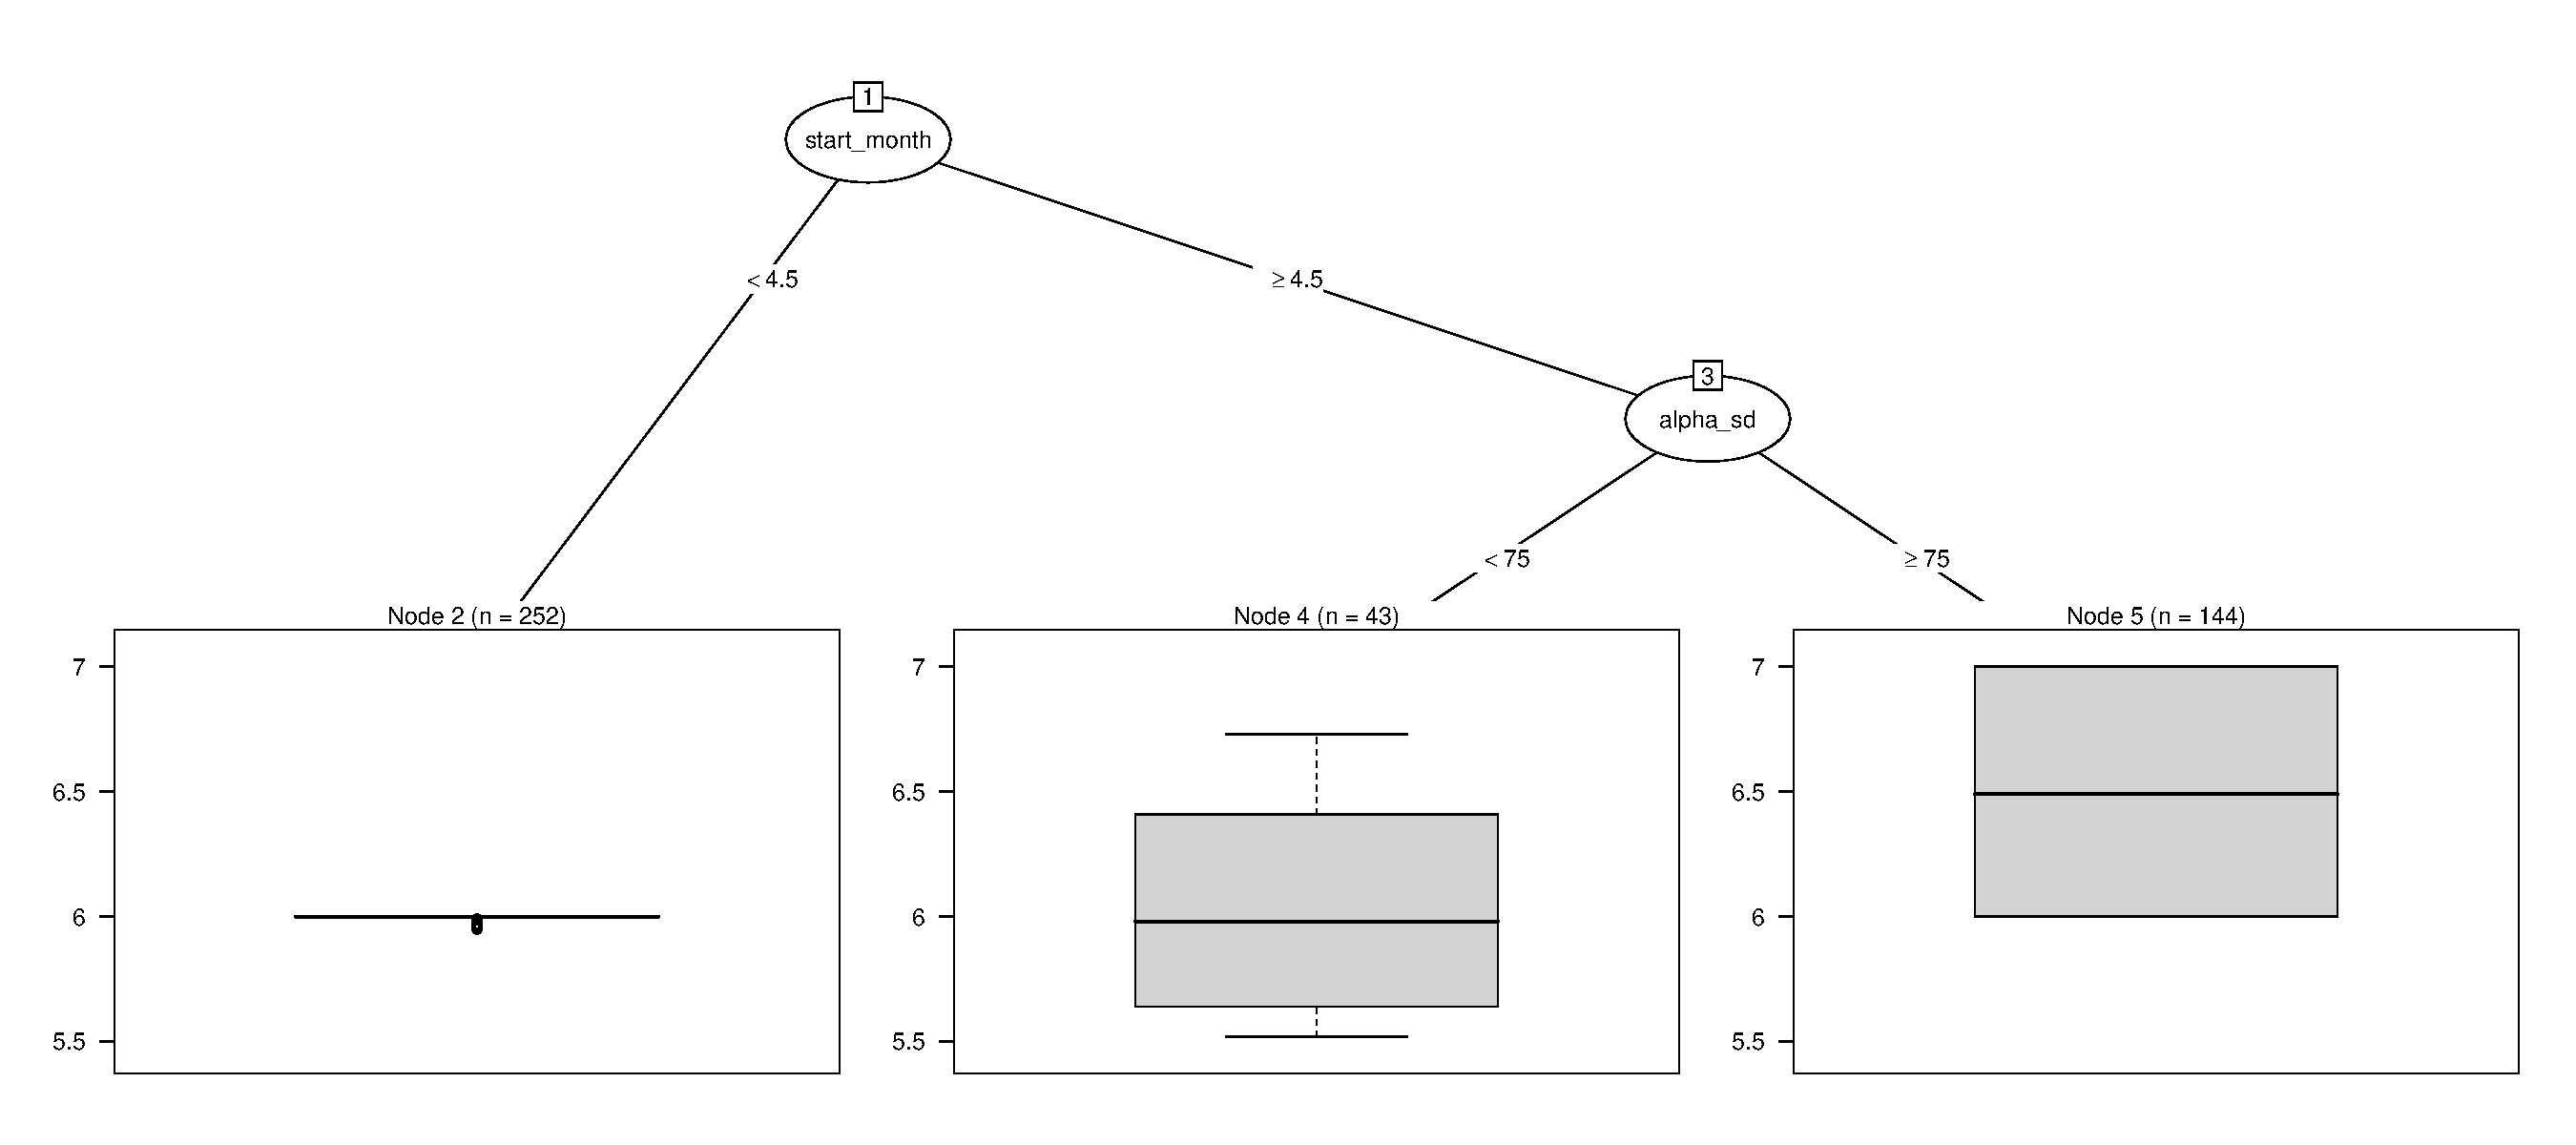
\includegraphics[width=\textwidth,trim={1cm 1cm 1cm 0cm},clip]{../cellular_automata/results/cart/m2_l1_tree.pdf}
\caption{$\mooreRange=2$, $\ell=1$}
    \end{subfigure}
    \begin{subfigure}[b]{.45\textwidth}
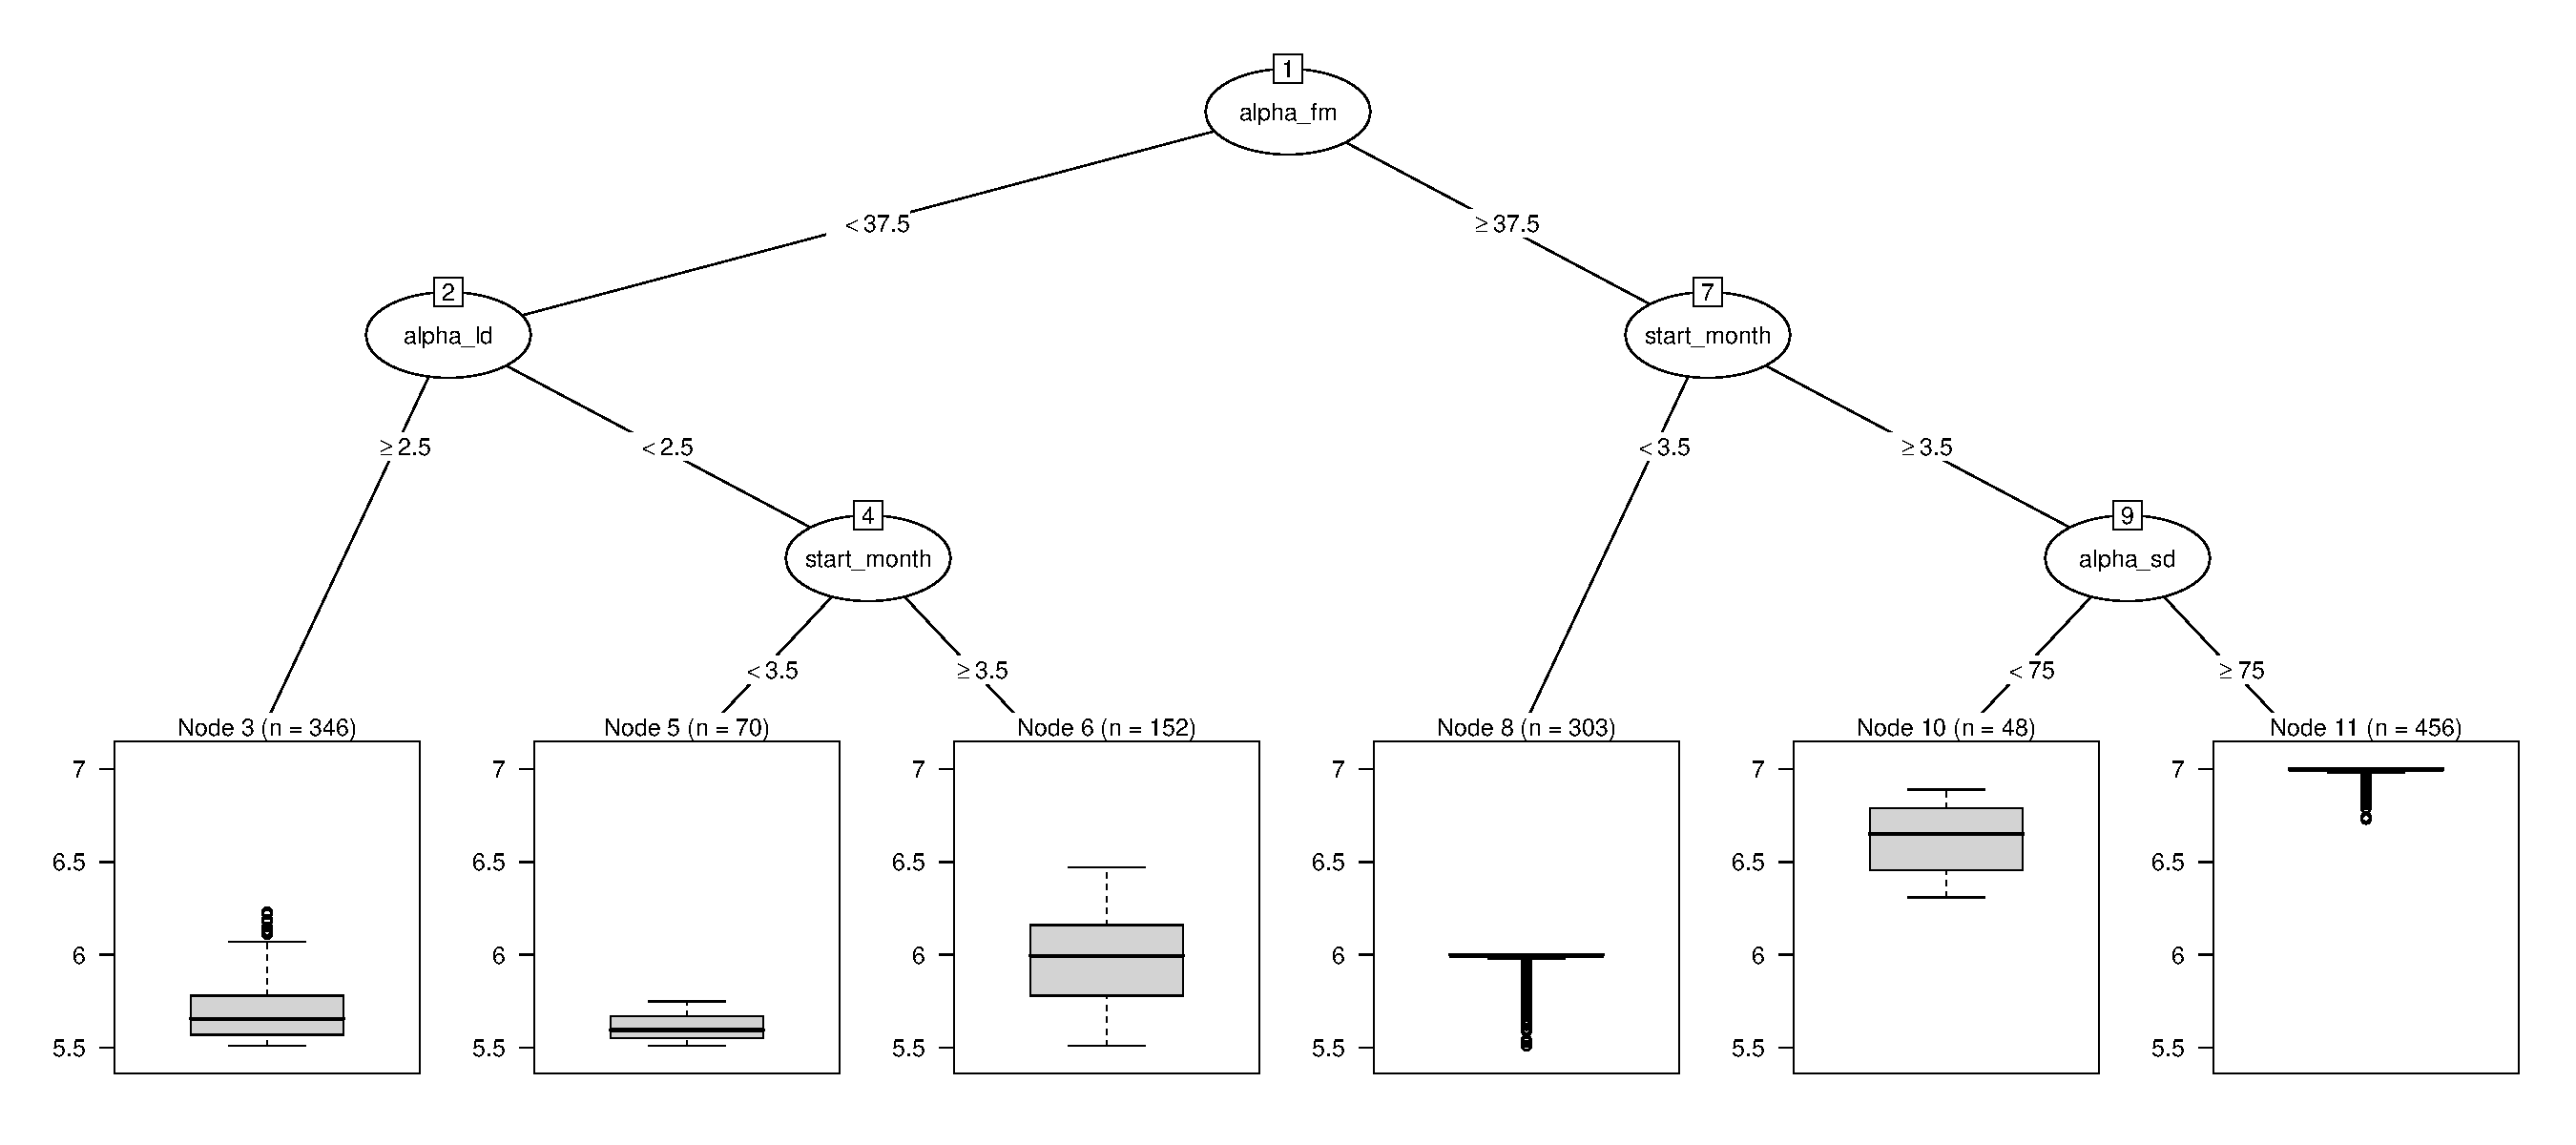
\includegraphics[width=\textwidth,trim={1cm 1cm 1cm 0cm},clip]{../cellular_automata/results/cart/m2_l2_tree.pdf}
\caption{$\mooreRange=2$, $\ell=2$}
    \end{subfigure}
    \begin{subfigure}[b]{.45\textwidth}
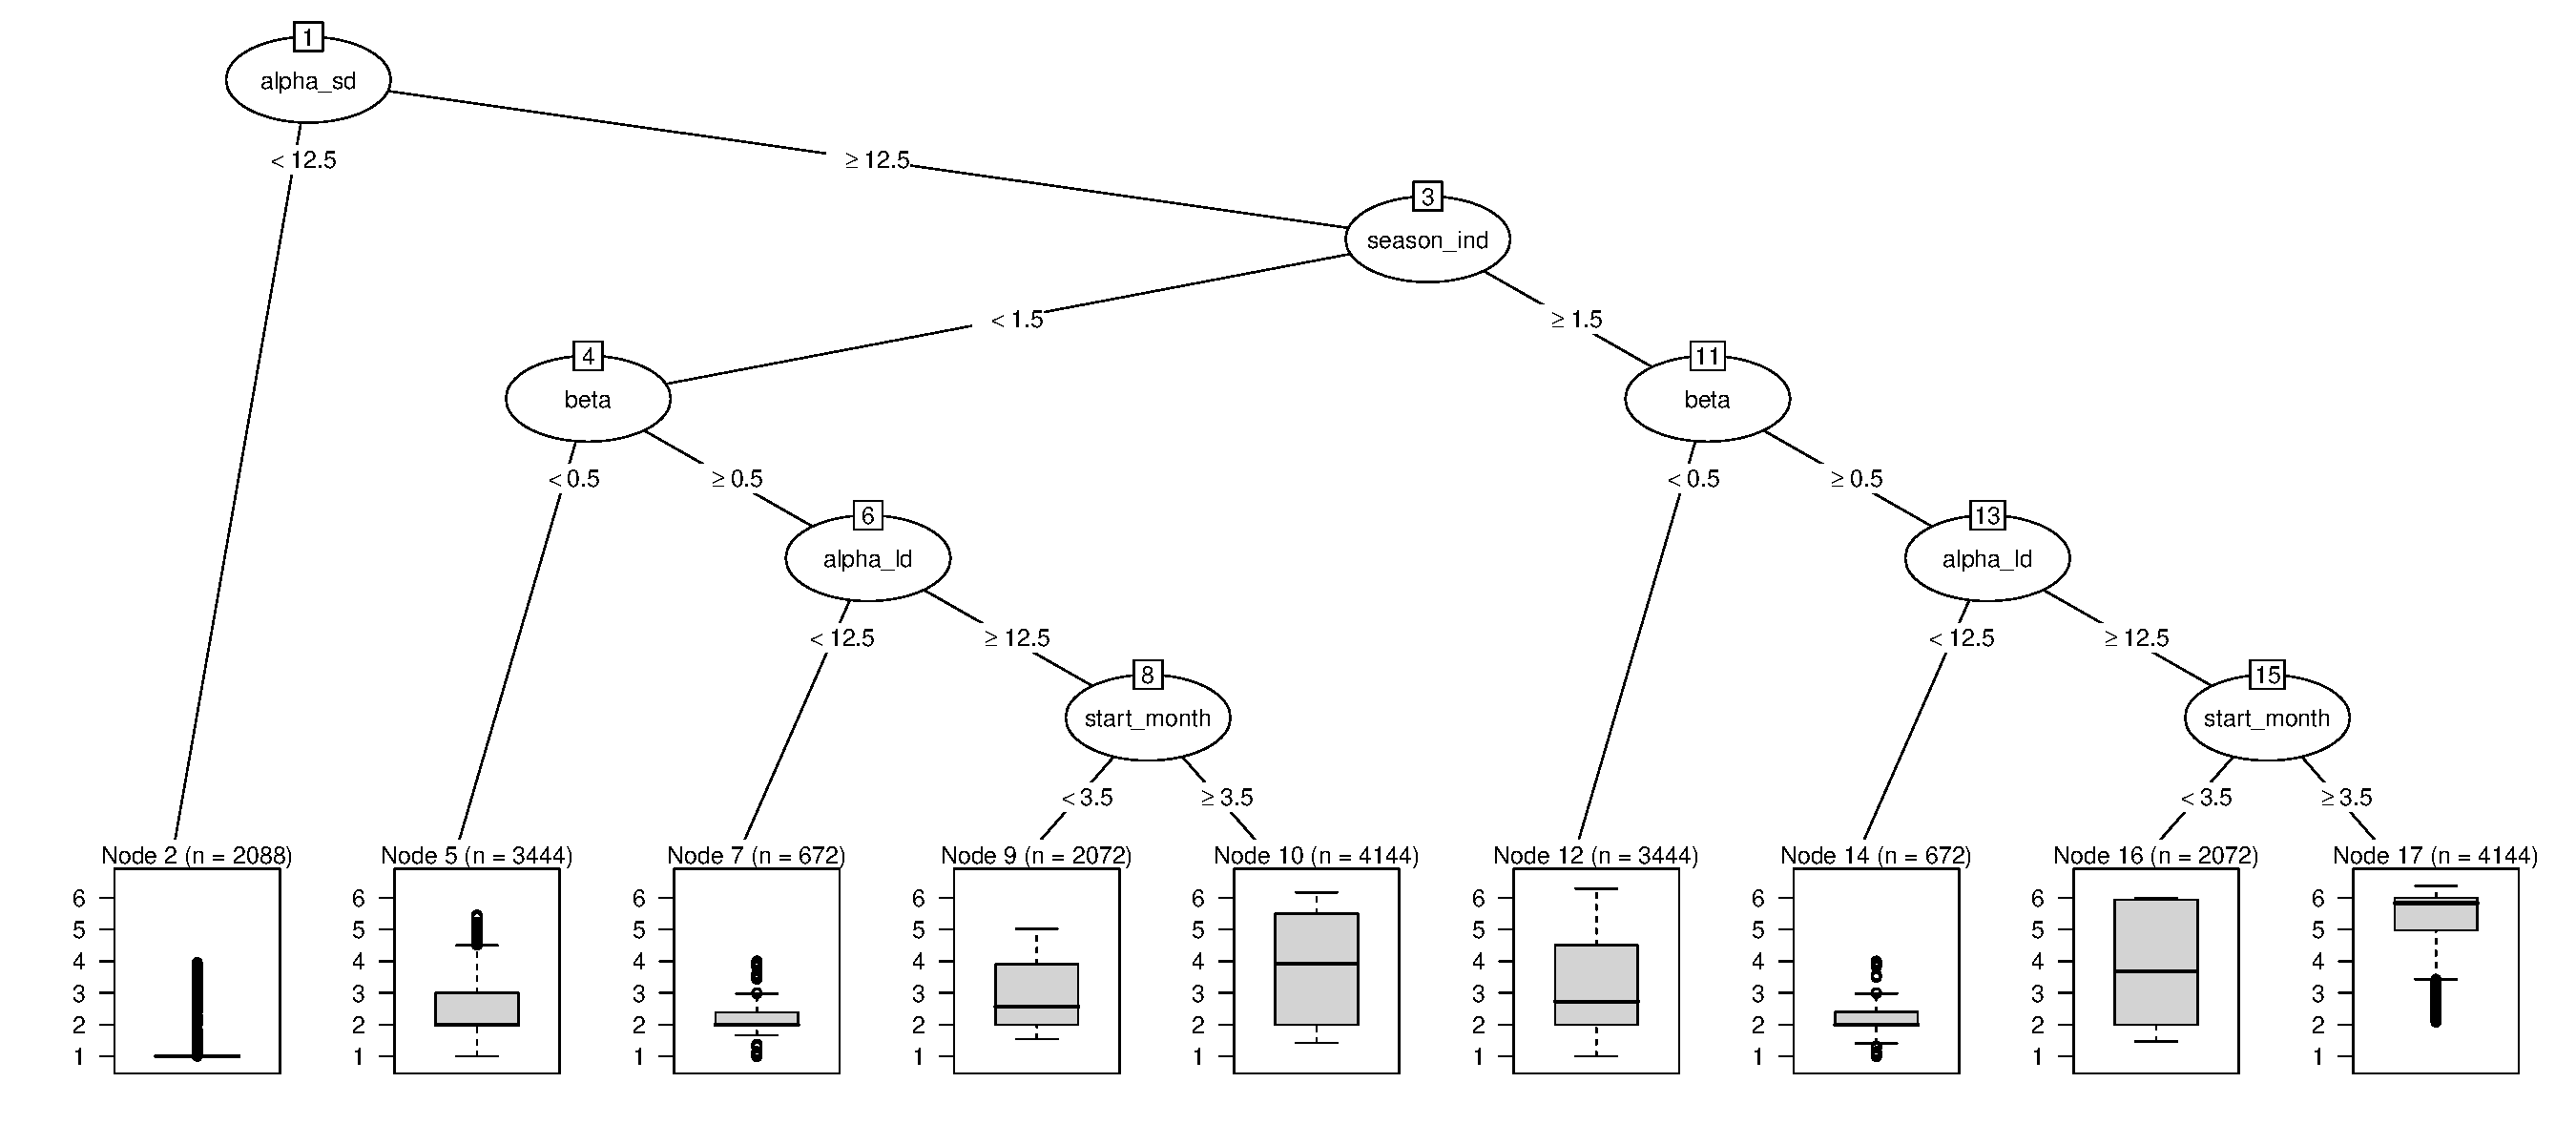
\includegraphics[width=\textwidth,trim={1cm 1cm 1cm 0cm},clip]{../cellular_automata/results/cart/m2_l3_tree.pdf}
\caption{$\mooreRange=2$, $\ell=3$}
    \end{subfigure}
%%     \begin{subfigure}[b]{.45\textwidth}
%% 
\includegraphics[width=\textwidth,trim={1cm 1cm 1cm 0cm},clip]{../cellular_automata/results/cart/m3_l1_tree.pdf}
%% \caption{$\mooreRange=3$, $\ell=1$}
%%     \end{subfigure}
    \begin{subfigure}[b]{.45\textwidth}
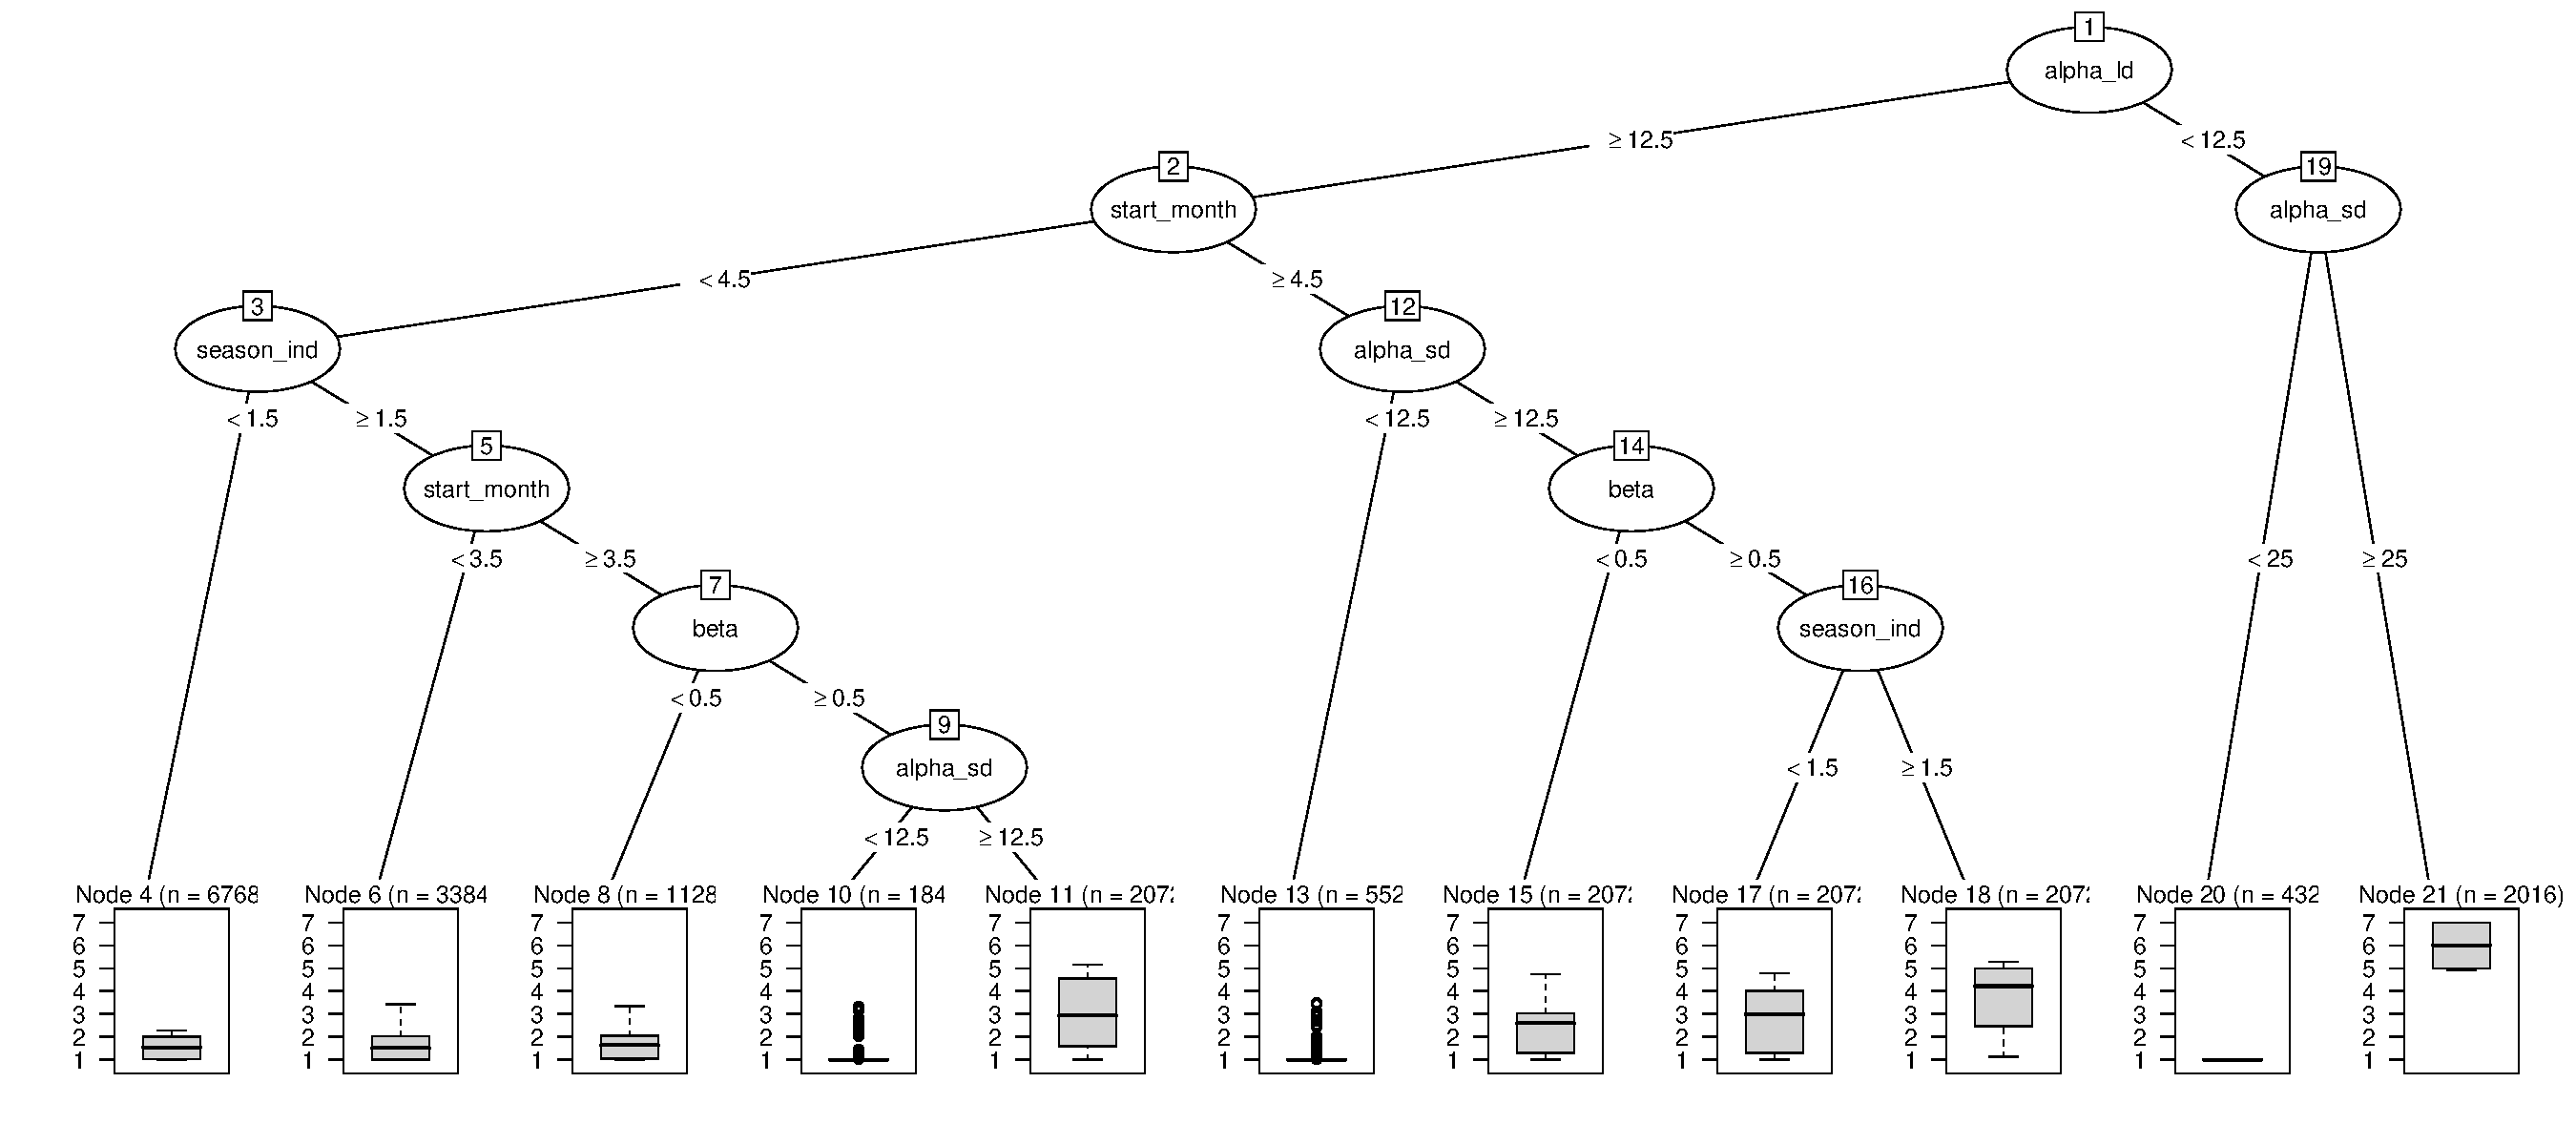
\includegraphics[width=\textwidth,trim={1cm 1cm 1cm 0cm},clip]{../cellular_automata/results/cart/m3_l2_tree.pdf}
\caption{$\mooreRange=3$, $\ell=2$}
    \end{subfigure}
    \begin{subfigure}[b]{.45\textwidth}
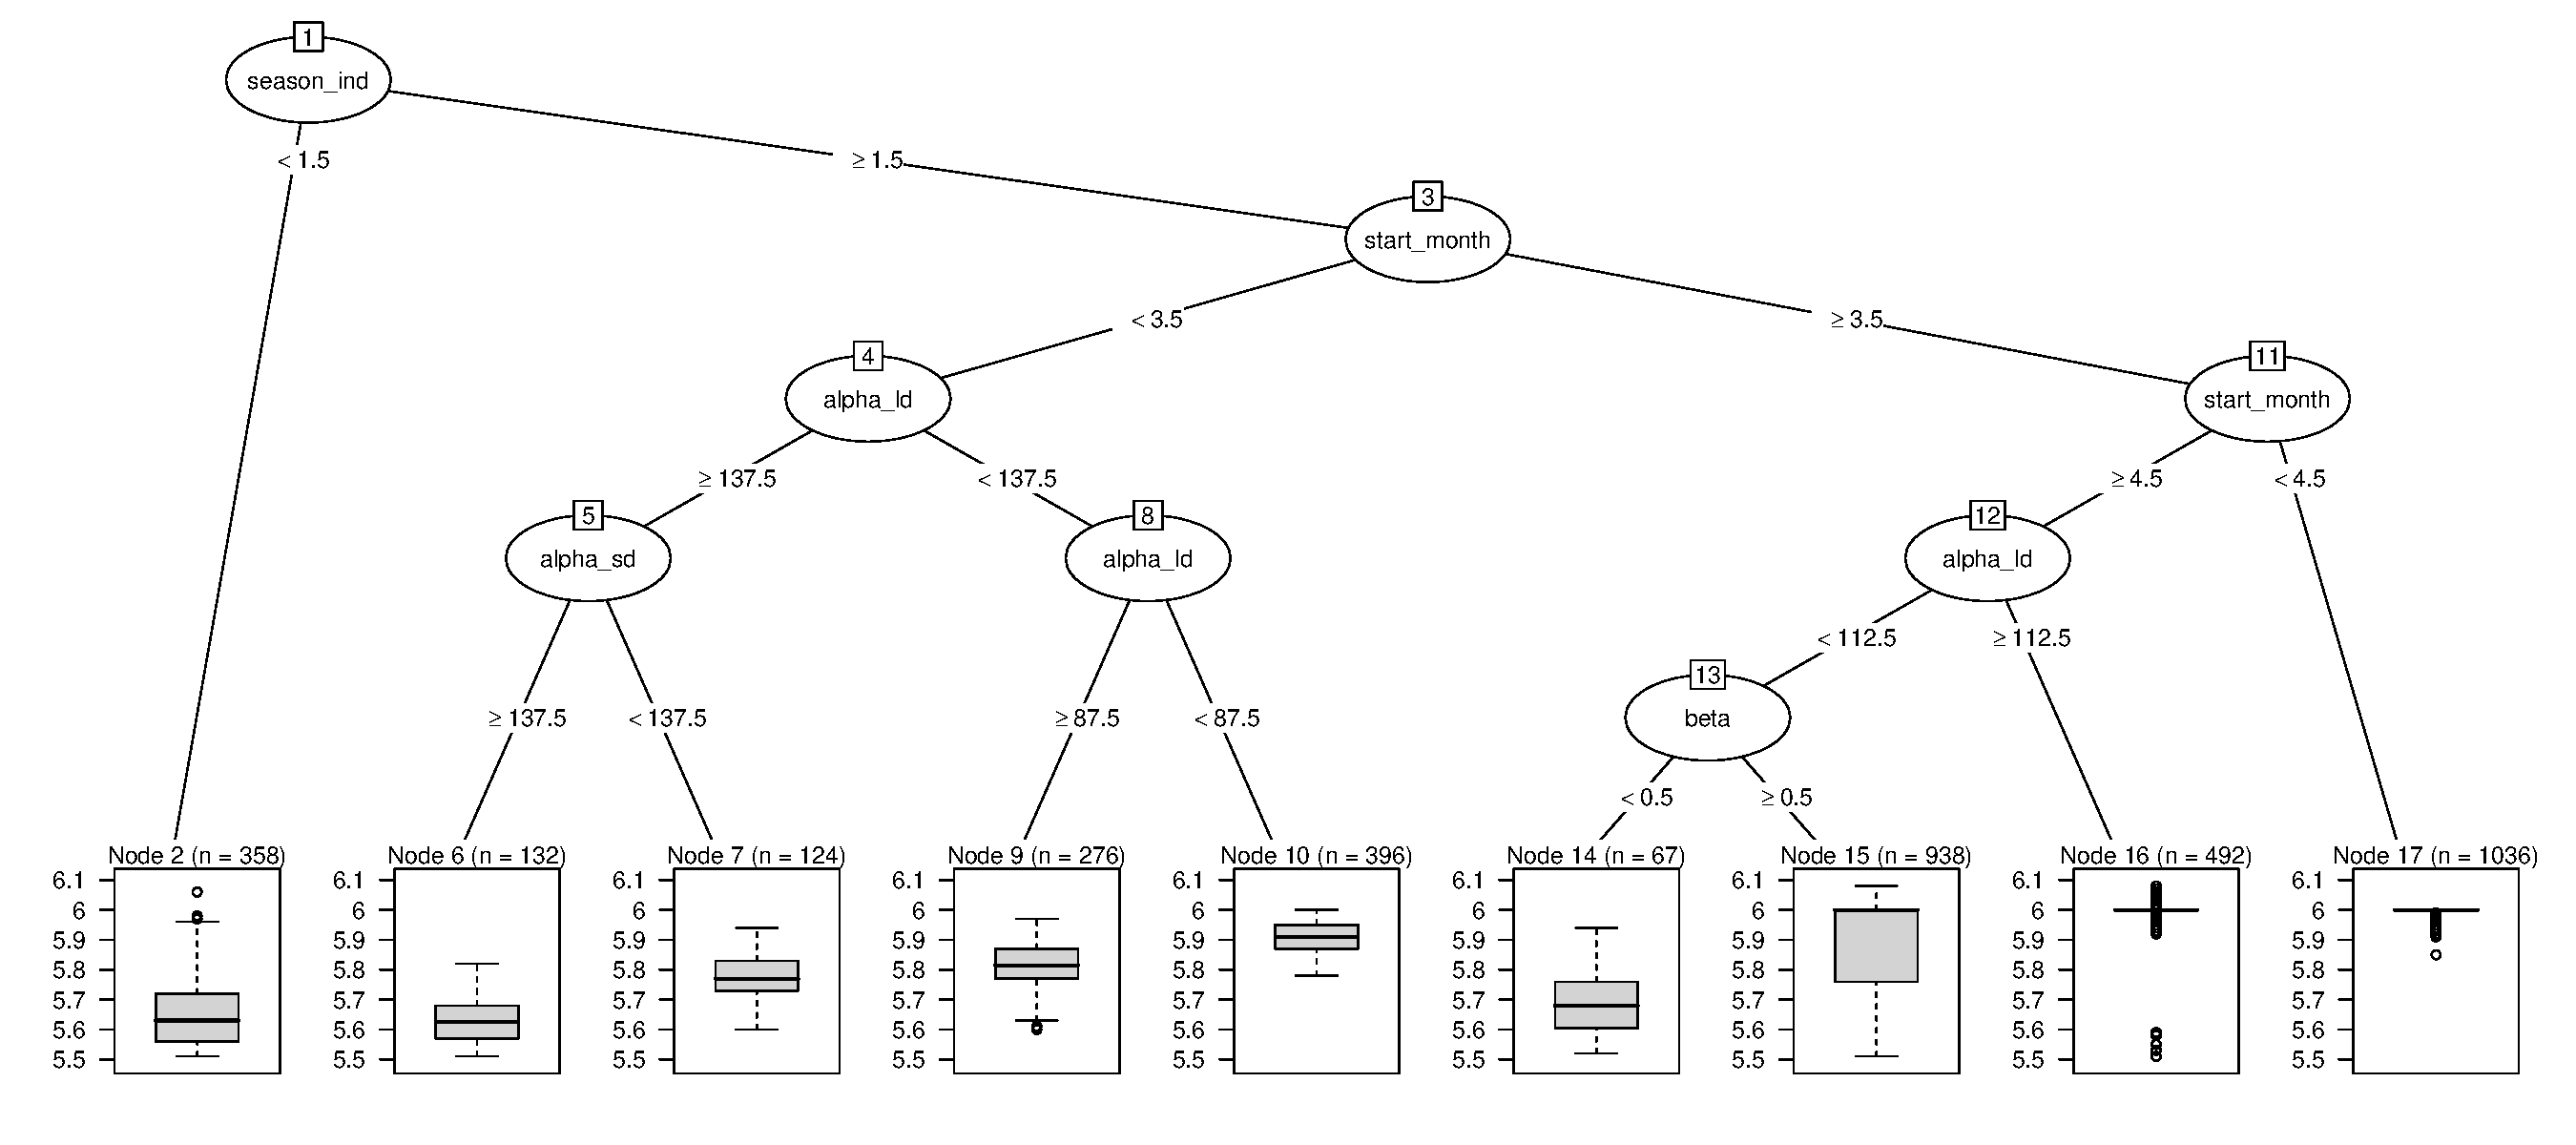
\includegraphics[width=\textwidth,trim={1cm 1cm 1cm 0cm},clip]{../cellular_automata/results/cart/m3_l3_tree.pdf}
\caption{$\mooreRange=3$, $\ell=3$}
    \end{subfigure}
    \caption{CART analysis of the parameter space: The models with
        similarity score~$\ge5.5$ were partitioned based on the Moore
    range~$\mooreRange$ and latency period~$\ell$ tuple and analysed. For
 the case~$(\mooreRange=3$, $\ell=1)$, there were no instances with
 similarity score~$\ge5.5$ among the sampled instances. 
    \label{fig:cart}}
\end{figure}

We recall that the emergent outcome of the model can be classified into two
classes: Class~A and Class~B. In Figure~\ref{fig:cart}, we show the results
of CART analysis on the parameter sets which yielded a similarity score of
$\ge5.5$. The chosen set is partitioned by Moore range~$\mooreRange$ and
latency period~$\ell$. For $(\mooreRange,\ell)$ values that permit rapid
range expansion through short-distance spread over the contiguous
landscape, including long-distance spread leads to faster spread than
observed leading to lower score. Hence, for those regimes, we
observe only Class~A spread. The corresponding~$(\mooreRange,\ell)$ values
are~$(1,1)$, $(2,1)$, $(2,2)$ and $(3,1)$. For the regime~$(3,1)$ we did
not observe any instance with score~$>5.5$.

\subsection{Seeding scenarios}
\label{sec:seeds}
During the model evaluation phase, to account for both spatial and temporal
observation noise, we considered six seeding scenarios: The locations
Bangladesh~1 and Bangladesh~2 (see Table~\ref{tab:seeds}) and start times
March, April or May (the month \tuta{} was reported).  For the prediction
phase, we constructed three different seeding scenarios reflecting three
different possible introductions to the region. The first corresponds to
spread from Bangladesh through northeast Myanmar. This region represents a
possible pathway of \tuta{} should it spread radially through the border
with Bangladesh. The second scenario we considered is the region of Johor
in Malaysia - including Singapore. This region contains major ports in
Malaysia including Tanjung Pelepas \cite{khalid2005}, and Singapore is also
a major trading hub for Bangladesh. We considered two scenarios of
introduction for Philippines. The first is motivated by the fact that there
is a large migrant Filipino worker population travelling to and from
infested countries. We seeded the port of Masinloc in this scenario as it
processes many of these travellers. The second was the introduction to
Northern Mindanao region, one of the major tomato production areas in the
country. We conducted country-specific experiments in the case of Thailand
and Vietnam. The seed locations were determined by spread observed from
both Class~A and Class~B models.
%% Scenario C seeded the region of
%% Putrajaya, which is the region which includes the largest port in Malaysia
%% \cite{khalid2005}. Scenario D seeded the region of Penang, which is also a
%% major port \cite{khalid2005}. 
%% Scenario E seeded Sarawak which is one of the
%% Malaysia districts not in the mainland. This district contains another
%% major port: Bintulu \cite{khalid2005}. When seeded in the mainland, the
%% Sarawak region is not reached with a Moore range of 2 or 3.This reflects
%% the natural spread of \tuta{} across the border of Myanmar. In this case we
%% seeded all cells northeast of a given boundary line, this is due to
%% uncertainty of the current distribution of the pest as well as likely
%% movement. The second scenario is an introduction through Singapore due to
%% trade. 
%%
\begin{table}[ht]
    \caption{Seeding scenarios\label{tab:seeds}}
    \centering
    \small
    \begin{tabular}{p{4cm} p{10cm}}
    	\hline
    	Region seeded & Description \\
    	\hline
    	\hline
        Bangladesh 1 & Parameterization phase: The cell corresponding to the location of first
        report was seeded. \\
        Bangladesh 2 & Parameterization phase: The cells corresponding to the location of first
        report and its adjacent cells (Moore neighbourhood~1) were seeded. \\
    	\hline
	Bangladesh and Northeastern Myanmar & This seeding is the estimated
	current range of \tuta{} in the study region. It is used to study
	the spread in the rest of the region.\\
    	\hline
    	Singapore and southern (mainland) Malaysia & This reflects possible introduction through trade, as Singapore is a major port.\\
    	\hline
    	Philippines 1 & This reflects the possibility of \tuta{} being
        introduced through workers travelling to and from India, and other
        countries, which have reported the pest. The port of Masinloc was
        seeded.\\
    	Philippines 2 & Northern Mindanao region\\
    	Thailand & Northwestern region: informed by observed spread in
        Mainland Southeast Asia.\\
    	Vietnam & Northwester region: Informed by observed spread in
        Mainland Southeast Asia.\\
    	\hline
    	\end{tabular}
\end{table}
\subsection{Software and Computational aspects.} The model was implemented
in Python~2.7. For data management and processing, we used PostGreSQL and
SQlite.  Statistical analysis was done using Python, R~3.4.3 and SPSS~24.0.
The experiments were run using Discovery, a high performance computing
cluster with 232 nodes (16-core Sandy Bridge-EP E5-2670 2.60GHz (3.30GHz
Turbo) Dual Processor (8 Cores per Processor) nodes with 32 GB of Memory
and 500 GB Internal Hard Drive) in the Biocomplexity Institute of Virginia~Tech.

\section{Clustering analysis of the spread pattern}
\label{sec:cluster}
We recall that each simulation output has the following format. Suppose,
the simulations were run for $T$ time steps. For every~$v$,~$p(v,t)$ is the
empirical probability  that cell $v$ is infected at time~$t$. Each
simulation output can be viewed as a matrix of size~$n\times T$, where~$n$
is the number of cells. To normalise each matrix, we introduced an extra
index~$T+1$ which carries the residual probability, i.e.,
$p(v,T+1)=\sum_{t=1}^Tp(v,t)$. The simulation outputs for models with
similarity $\similarity\ge6$ were thus processed and clustered using two
algorithms: hierarchical
agglomerative clustering (SPSS 24.0) and $k$-means algorithm (using
Pyclustering~\cite{andrei_novikov_2018_1491324}). In each case, the number of
clusters considered ranged from~$k=1$ to~$10$. 

To discover relationships between model parameters and cluster membership,
we cast it as a classification problem. With configurations as features and
cluster index as labels, we applied CART. The resulting decision tree was
used to interpret the relationship between parameters and cluster
membership. The results are in Figures~\ref{fig:cartAgglomerative}
(hierarchical) and~\ref{fig:cartkmeans} ($k$-means).

%%
\begin{figure}[pht]
\centering
\begin{subfigure}[b]{.6\textwidth}
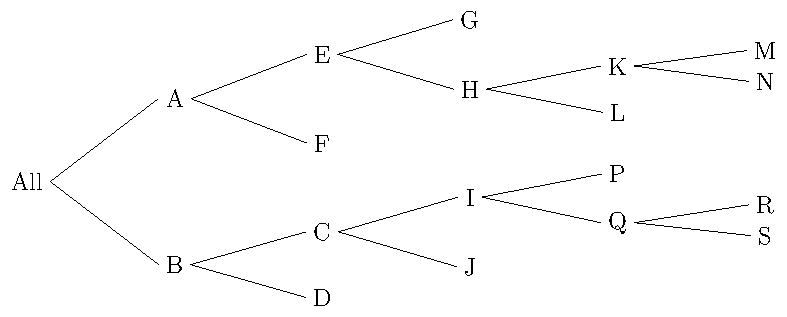
\includegraphics[width=\textwidth]{../clustering/results/agglomerative/hierarchy_agglomerative.pdf}
\caption{Hierarchy}
\end{subfigure}
%%
\begin{subfigure}[b]{.32\textwidth}
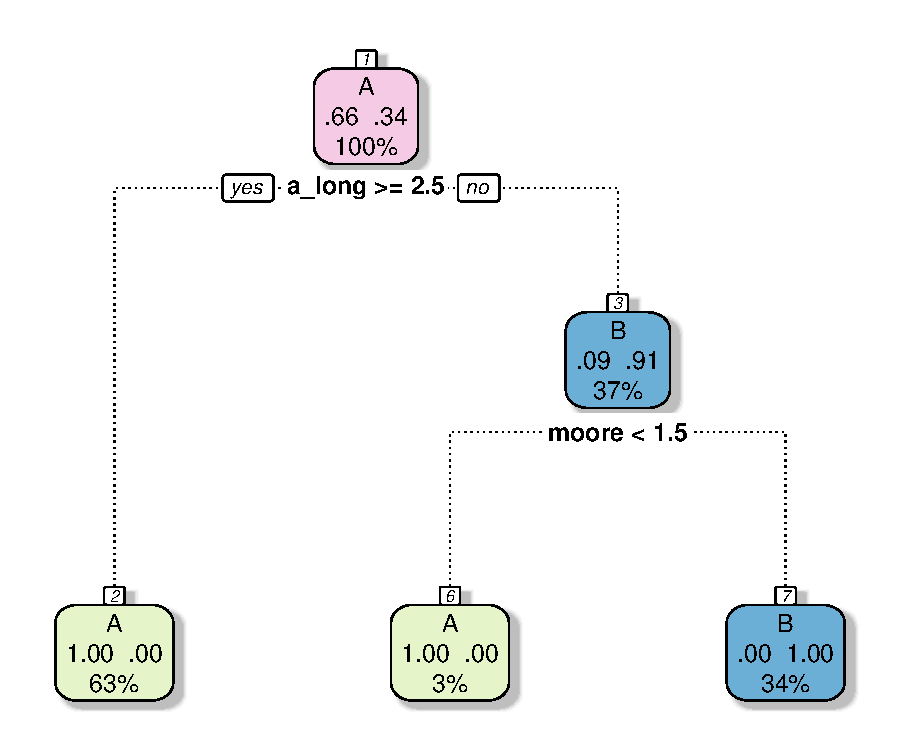
\includegraphics[width=\textwidth]{../clustering/results/agglomerative/cart_cAB_agg.pdf}
\caption{$k=2$}
\end{subfigure}
%%
\begin{subfigure}[b]{.32\textwidth}
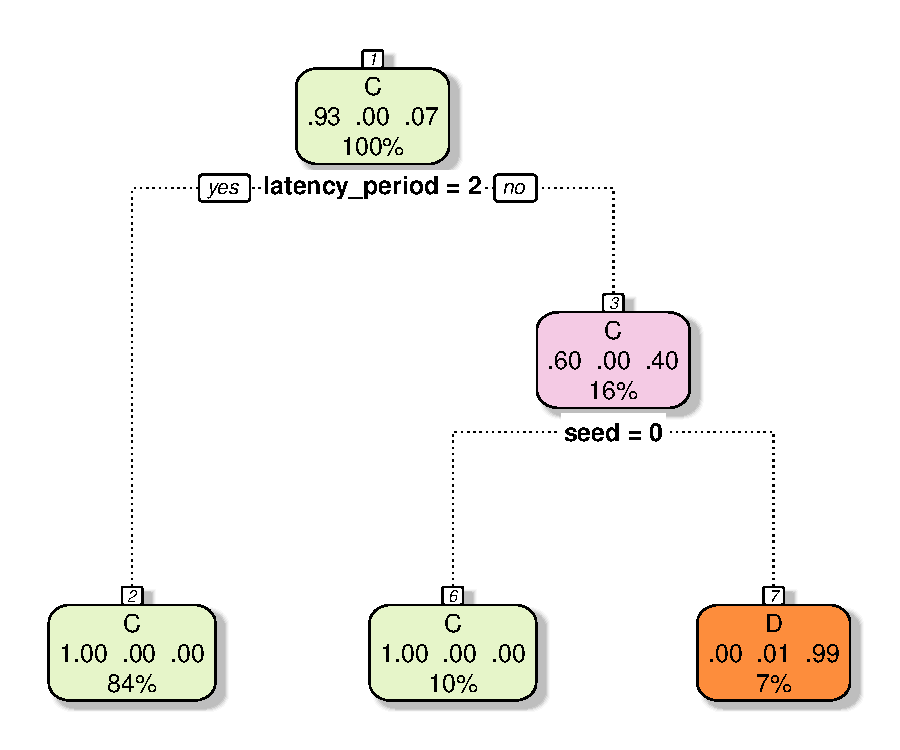
\includegraphics[width=\textwidth]{../clustering/results/agglomerative/cart_cCD_agg.pdf}
\caption{$k=3$}
\end{subfigure}
%%
\begin{subfigure}[b]{.32\textwidth}
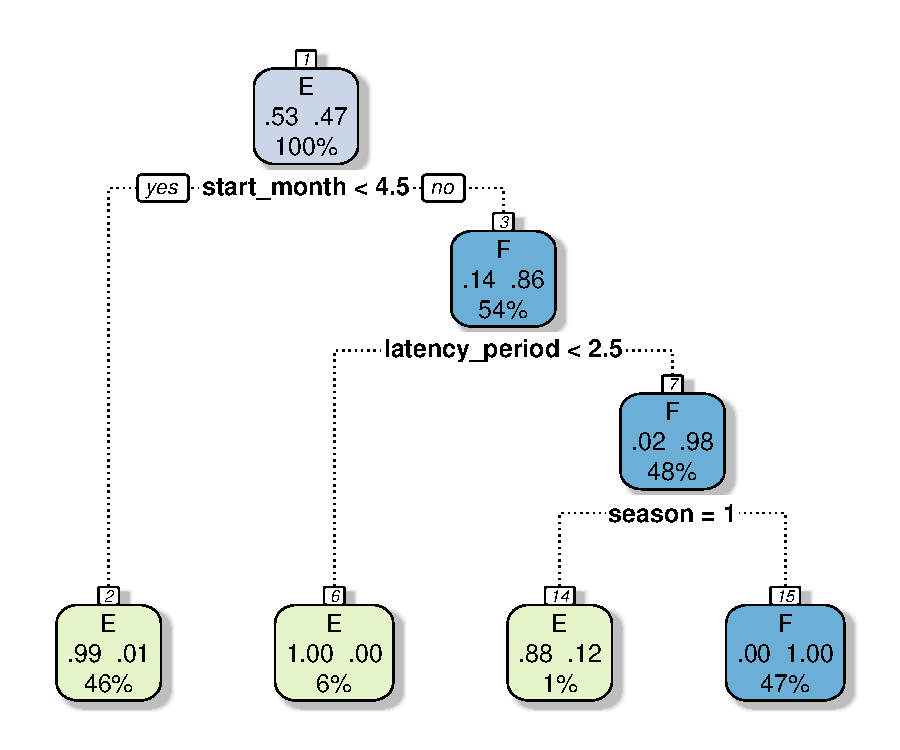
\includegraphics[width=\textwidth]{../clustering/results/agglomerative/cart_cEF_agg.pdf}
\caption{$k=4$}
\end{subfigure}
%%
\begin{subfigure}[b]{.32\textwidth}
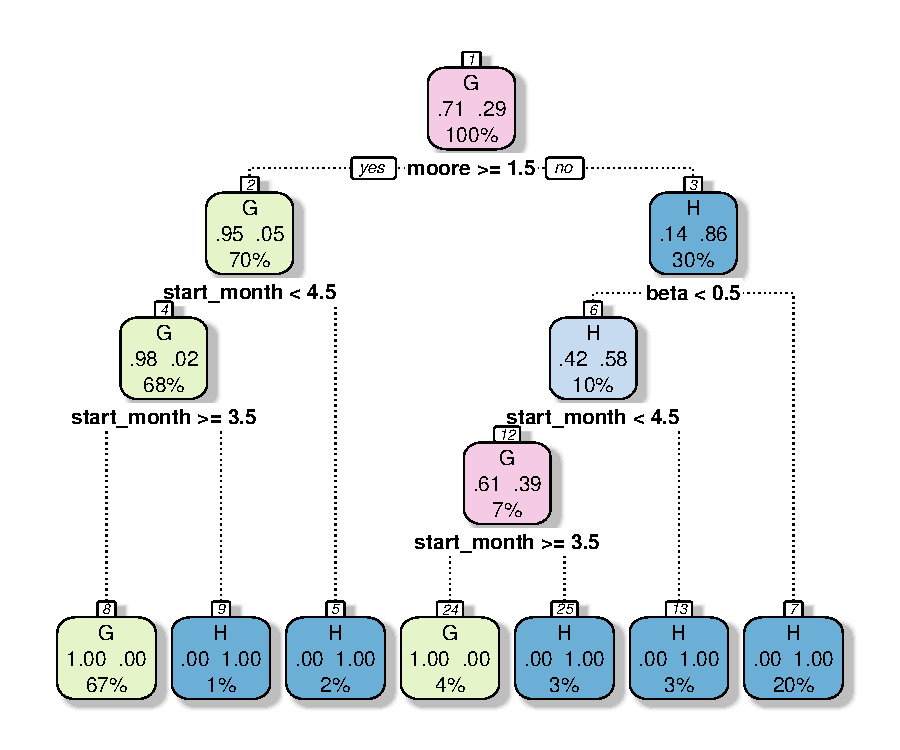
\includegraphics[width=\textwidth]{../clustering/results/agglomerative/cart_cGH_agg.pdf}
\caption{$k=5$}
\end{subfigure}
%%
\begin{subfigure}[b]{.32\textwidth}
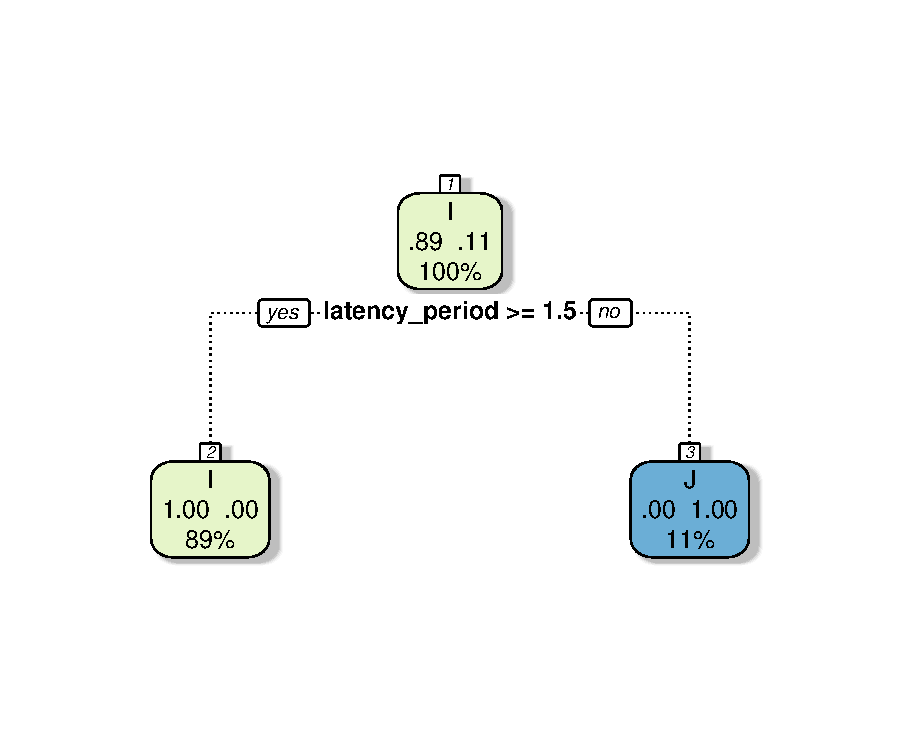
\includegraphics[width=\textwidth]{../clustering/results/agglomerative/cart_cIJ_agg.pdf}
\caption{$k=6$}
\end{subfigure}
%%
\begin{subfigure}[b]{.32\textwidth}
\includegraphics[width=\textwidth]{../clustering/results/agglomerative/cart_cKL_agg.pdf}
\caption{$k=7$}
\end{subfigure}
%%
\begin{subfigure}[b]{.32\textwidth}
\includegraphics[width=\textwidth]{../clustering/results/agglomerative/cart_cMN_agg.pdf}
\caption{$k=8$}
\end{subfigure}
%%
\begin{subfigure}[b]{.32\textwidth}
\includegraphics[width=\textwidth]{../clustering/results/agglomerative/cart_cPQ_agg.pdf}
\caption{$k=9$}
\end{subfigure}
%%
\begin{subfigure}[b]{.32\textwidth}
\includegraphics[width=\textwidth]{../clustering/results/agglomerative/cart_cRS_agg.pdf}
\caption{$k=10$}
\end{subfigure}
%%
\caption{\textbf{Agglomerative clustering of simulation outputs.} The
9-level hierarchy of the clusters is shown in (a). At each level, we
applied CART to understand which parameter was significantly influencing
the split. Here, \texttt{a\_long} corresponds to $\ald$,
\texttt{latency\_period} is~$\ell$ and \texttt{moore} is $\mooreRange$.
\label{fig:cartAgglomerative}}
\end{figure}

%%
\begin{figure}[pht]
\centering
%%
\begin{subfigure}[b]{.47\textwidth}
\includegraphics[width=\textwidth]{../clustering/results/kmeans/cart_kmeans_2.pdf}
\caption{$k=2$}
\end{subfigure}
%% %%
%% \begin{subfigure}[b]{.32\textwidth}
%% \includegraphics[width=\textwidth]{../clustering/results/kmeans/cart_kmeans_3.pdf}
%% \caption{$k=3$}
%% \end{subfigure}
%% %% %%
%% \begin{subfigure}[b]{.32\textwidth}
%% \includegraphics[width=\textwidth]{../clustering/results/kmeans/cart_kmeans_4.pdf}
%% \caption{$k=4$}
%% \end{subfigure}
%% %%
\begin{subfigure}[b]{.47\textwidth}
\includegraphics[width=\textwidth]{../clustering/results/kmeans/cart_kmeans_5.pdf}
\caption{$k=5$}
\end{subfigure}
%% %%
%% \begin{subfigure}[b]{.32\textwidth}
%% \includegraphics[width=\textwidth]{../clustering/results/kmeans/cart_kmeans_6.pdf}
%% \caption{$k=6$}
%% \end{subfigure}
%% %%
%% \begin{subfigure}[b]{.32\textwidth}
%% \includegraphics[width=\textwidth]{../clustering/results/kmeans/cart_kmeans_7.pdf}
%% \caption{$k=7$}
%% \end{subfigure}
%% %%
%% \begin{subfigure}[b]{.32\textwidth}
%% \includegraphics[width=\textwidth]{../clustering/results/kmeans/cart_kmeans_8.pdf}
%% \caption{$k=8$}
%% \end{subfigure}
%% %%
%% \begin{subfigure}[b]{.32\textwidth}
%% \includegraphics[width=\textwidth]{../clustering/results/kmeans/cart_kmeans_9.pdf}
%% \caption{$k=9$}
%% \end{subfigure}
%%
\begin{subfigure}[b]{.6\textwidth}
\includegraphics[width=\textwidth]{../clustering/results/kmeans/cart_kmeans_10.pdf}
\caption{$k=10$}
\end{subfigure}
%%
\caption{\textbf{$k$-means clustering of simulation outputs.} For each $k$,
the number of clusters, we applied CART to understand which parameter was
significantly influencing the split. Here, \texttt{a\_long} corresponds to
$\ald$, \texttt{latency\_period} is~$\ell$ and \texttt{moore} is
$\mooreRange$.
\label{fig:cartkmeans}}
\end{figure}
\section{More results}
\subsection{International trade} \label{sec:tomnet}
Figure~\ref{fig:tomnet} shows the annual tomato trade for the study region. The
network was constructed using data from FAOSTAT Trade matrix
(Table~\ref{tab:data}).  The trade within the focus region is represented
by green edges. Imports from \tuta{} affected countries categorised by
region is represented by red edges, and the blue edges correspond to
exports from the focus region to countries yet to report the presence of
the pest. The edge thickness is a function of the trade volume. We note
that with the exception of Philippines, there is considerable trade
activity among countries in the focus region. However, the majority of
trading happens between neighbouring countries and except for a few flows,
the volume is negligible compared to production within. Most significant
flow is from Malaysia to Singapore ($\approx30,000$ tonnes), India to
Bangladesh ($\approx20,000$ tonnes), and Thailand and Vietnam to Malaysia
(between $1000$ to $2,000$ tonnes). Philippines does not report any fresh
tomato trade with other countries.  We also analysed how the network
structure evolved across years. While we did not observe much variation in
the network structure, there is some change in the countries importing to
and exporting from this region
%%
\begin{figure}[ht]
\centering
%%
\begin{subfigure}[b]{.47\textwidth}
\includegraphics[width=\textwidth]{../international_trade/results/network_plots/sea_2013_tomato.pdf}
\caption{Tomato trade in the focus region (2013).\label{fig:tomnet}}
\end{subfigure}
%%
\begin{subfigure}[b]{.47\textwidth}
\includegraphics[width=\textwidth]{../international_trade/results/stat_plots/trends.pdf}
\caption{General trends of overall production and trade in the region over
a decade based on FAOSTAT 2013.  \label{fig:trends}}
\end{subfigure}
%%
\begin{subfigure}[b]{\textwidth}
\includegraphics[width=.32\textwidth]{../international_trade/results/network_plots/sea_2011_tomato.pdf}
\includegraphics[width=.32\textwidth]{../international_trade/results/network_plots/sea_2012_tomato.pdf}
\includegraphics[width=.32\textwidth]{../international_trade/results/network_plots/sea_2013_tomato.pdf}
\caption{Evolution over years 2011, 2012, 2013. \label{fig:tradeYears}}
\end{subfigure}

\end{figure}

\paragraph{General trends.} Figure~\ref{fig:trends} shows the evolution of
trade and production volume over time. The total tomato production in
the study region obtained by summing the production for all countries is
plotted for each year between~2004 to~2013 (blue). We computed the total
tomato import volume per year (green) from outside the study region using
FAOSTAT Trade Matrix (Table~\ref{tab:data}). This was obtained by
aggregating imports where the importing country belongs to the study region
and the exporting country is outside the region. Similarly export volume
per year to outside the study region (red) is shown. Finally, the amount of
tomato traded within the study region was obtained by aggregating tomato
trade between countries in the region for each year (orange). In order to
compare these plots, each plot was normalised by dividing by the
corresponding maximum value across all years.
There is a steady
increase in the production and amount of internal trade, with comparable
rate of change for both quantities.  In comparison, the export of tomato to
outside of the focus region (plot ``Exports'') has risen steeply in the
recent years (after 2011), while the imports generally indicate a downward trend (plot
``Imports''). Recent efforts to increase production and trade
infrastructure in these countries support these 
trends~\cite{huong2013,buntong2013,moustier2007}.
Under these circumstances, \tuta{}'s invasion can have a high negative
impact on the economy and livelihood of the people in this region.


\subsection{Localities, production and trade}
\label{sec:locality_flows}
We identified 102 localities representing urban and production centres. For
the purpose of this discussion, a \emph{major source} (\emph{major sink})
is a locality with net outflow (inflow) at least 10~Kilo tonnes. Among
these, less than 20\% of the localities have net outflow of at least
10~Kilo tonnes in the gravity model derived trade network, indicating that
there are few major sources (Figure~\ref{fig:prod_netout}).  We also note
that there are a few high sinks which have production comparable to some of
the major sources.  These are regions not only vulnerable to attacks, but
also potentially sustain a huge negative impact due to loss in production.

To predict seasonal production, we used linear regression to model the
production rate as a function of precipitation, temperature, and elevation
using seasonal production data from different regions of Philippines. The
results showed that precipitation was a statistically significant predictor
($p<0.001$). More details are in Section~\ref{sec:prod} in the supplement.
To study the effect of seasonality on monthly flows, we accumulated the net
flow per month by directionality. For a locality~$i$, let~$F_i(m)$ denote
the net flow in month~$m$ (positive means outflow, else inflow). The
accumulated outflow is $F_i^+=\sum_{m=1}^{12} I\big(F_i(m)>0\big)F_i(m)$,
where~$I(\cdot)$ is the indicator function. Corresponding definition of
accumulated inflow is $F_i^-=\sum_{m=1}^{12} I\big(F_i(m)<0\big)F_i(m)$.
The results in Figure~\ref{fig:monthly_in_out} show that there are very few
localities which switch from the role of source to sink and vice versa.
This is unlike what is observed in Nepal by
Venkatramanan~et~al.~\cite{venkatramanan2019modeling}. The flow between
high altitude regions and low altitude regions switches direction according
to season.  Here, while the intensity of flows vary between seasons, we do
not see such a switch in roles.

%%
\begin{figure}[ht]
    \centering
\begin{subfigure}[b]{.47\textwidth}
    \includegraphics[width=\textwidth]{../long_distance/results/prod_netout_flows_precip1_b2_k500.pdf}
    \caption{Net annual production and outflow\label{fig:prod_netout}}
\end{subfigure}\hspace{.5cm}
\begin{subfigure}[b]{.47\textwidth}
    \includegraphics[width=\textwidth]{../long_distance/results/monthly_in_out_flows_precip1_b2_k500.pdf}
    \caption{Effect of seasonality on monthly flows\label{fig:monthly_in_out}}
\end{subfigure}
\caption{\textbf{Production, inflow and outflow at localities.} These are
results for $\beta=2$ and $\kappa=500$ (i) \label{fig:tradeProps}}
\end{figure}
%% %%   
%%
\begin{figure}[t]
\centering
\begin{subfigure}[b]{\textwidth}
    \includegraphics[width=0.47\textwidth]{../cellular_automata/results/rf/rf_importance_all_mdi.pdf}
    \includegraphics[width=0.47\textwidth]{../cellular_automata/results/rf/rf_importance_all_mse.pdf}
    \caption{Similarity score ($\similarity$) based evaluation. \label{fig:rfA}}
\end{subfigure}
\begin{subfigure}[b]{\textwidth}
    \includegraphics[width=0.47\textwidth]{../clustering/results/agglomerative/rf_k_agglomerative_mse.pdf}
    \includegraphics[width=0.47\textwidth]{../clustering/results/agglomerative/rf_k_agglomerative_mdg.pdf}
    \caption{Agglomerative clustering\label{fig:rfA}}
\end{subfigure}
\begin{subfigure}[b]{\textwidth}
    \includegraphics[width=0.47\textwidth]{../clustering/results/kmeans/rf_k_kmeans_mse.pdf}
    \includegraphics[width=0.47\textwidth]{../clustering/results/kmeans/rf_k_kmeans_mdg.pdf}
    \caption{$k$-means clustering\label{fig:rfA}}
\end{subfigure}
\caption{\textbf{Parameter importance.}\label{fig:rf}}
\end{figure}
%%
\subsection{Cellular automata model from Guimapi~et~al}
\label{sec:guimapi}
Guimapi~et~al.~\cite{guimapi2016modeling} use a cellular automata approach
to model the spread of \tuta{} through the study region of Africa, Spain, and Portugal. 
Here, we implemented and applied the model to study the spread in the focus
region.
%%
\paragraph{Methodology.}
Each cell in the automata is of size $25\mathrm{km}\times25\mathrm{km}$ induced by a
grid overlayed on the study region. Both square and hexagonal cell
configurations are considered, but square cells (Moore neighbourhood) were
chosen in order to cover a larger area per cell.
Each cell can be in one of three states: S, E and I with very similar
definitions as in our model.
The spread is modelled as follows:
For an infected cell to spread to another, each cell within its moore
neighbourhood of respective distance is considered in each time step (one month). If this neighbour cell is
suitable, it will change states. The suitability of a cell for pest
establishment depends on temperature, humidity, NDVI, and tomato production
in that cell at the given time step.
%\aacomment{Need to say what each time step corresponds to} 
Two Moore neighbourhoods were
considered, one with a range of 50 km and another with a range of 75 km.
%\aacomment{I don't think they claim that theirs is a natural spread model.
%Correct me if I am wrong.}

Given a cell within the Moore neighbourhood of an infected cell, its state
in the next time step depends on the following rules.
\begin{itemize} 
\item If NDVI $\ge$ NDVI threshold 1, then state becomes "Exposed".
\item If NDVI $\ge$ NDVI threshold 1 and temperature $>=$ temperature threshold and humidity $>=$ humidity threshold, then state becomes "Invaded".
\item If NDVI $\ge$ NDVI threshold 2 and tomato production high or very high, then state becomes "Invaded".
\item Otherwise the state remains unchanged
\end{itemize}

%\aacomment{refer to figure in paper, remove figure from here}.
%\noindent
%% Figure 2 in \cite{guimapi2016modeling} gives these rules for changing states.
%\begin{figure}[ht]
%        \centering
%        \includegraphics[width=\textwidth]{figs/Guimapi_fig.png}
%        \caption{Rules for changing states}
%        \label{Guimapi_rules}
%\end{figure}
Temperature, humidity, and NDVI data is at the level of the cell, while
production data is at the country-level. The temperature threshold is 22
degrees Celsius and humidity threshold is 55\%. The NDVI threshold 1 is
0.1, and threshold 2 is 0.3. The production yield threshold is 10
tons/hectare to be considered high or very high. Thus if a cell is within a
country with high or very high yield, that cell would be classified at high
or very high yield.
\paragraph{Results.}
We applied the seeding scenarios described in Table~\ref{tab:seeds}. Each
scenario was simulated with Moore neighbourhoods of~2 and~3.  The results
are shown in Figure~\ref{fig:baselineMyanmar}.  The model predicts a rapid
radial spread in this region as vegetation and temperature are generally
favourable throughout this region.  The tomato production yield in each
country in the focus region is in the high or very high categories, and
thus did not limit the spread.  Generally, the predicted range expansion is
much faster compared to our models, particularly in the case where Moore
range is~3.

\begin{figure}[ht]
    \begin{subfigure}[b]{.48\textwidth}
\centering
\includegraphics[width=\textwidth]{figs/plot_Myanmar2.pdf}
\caption{Moore neighbourhood of 2}
\end{subfigure}
\begin{subfigure}[b]{.48\textwidth}
\centering
\includegraphics[width=\textwidth]{figs/plot_Myanmar3.pdf}
\caption{Moore neighbourhood of 3, baseline model}
\end{subfigure}
\caption{Guimapi~et~al.~\cite{guimapi2016modeling} model results: 
Here the region of Chin in northeast Myanmar was seeded.
    \label{fig:baselineMyanmar}}
\end{figure}
\begin{figure}[htb]
%% \begin{subfigure}[b]{.47\textwidth}
%%     \includegraphics[width=\textwidth]{../cellular_automata/results/dist_inf_plots/dist_prob_B_moore.pdf}
%%     \caption{Model~A\label{fig:spreadRateMooreA}}
%% \end{subfigure}
%% %%
%% \begin{subfigure}[b]{.47\textwidth}
%%     \includegraphics[width=\textwidth]{../cellular_automata/results/dist_inf_plots/dist_prob_B_moore.pdf}
%%     \caption{Model~B\label{fig:spreadRateMooreB}}
%% \end{subfigure}
%% %%
\begin{subfigure}[b]{.47\textwidth}
    \includegraphics[width=\textwidth]{../cellular_automata/results/dist_inf_plots/dist_prob_A_box.pdf}
    \caption{Class~A\label{fig:spreadRateA}}
\end{subfigure}
%%
\begin{subfigure}[b]{.47\textwidth}
    \includegraphics[width=\textwidth]{../cellular_automata/results/dist_inf_plots/dist_prob_B_box.pdf}
    \caption{Class~B\label{fig:spreadRateB}}
\end{subfigure}
\caption{\textbf{Spread in Mainland Southeast Asia with respect to distance
from origin.} The cells are binned based on their distance from the origin
of infection (Northern Myanmar). Given time step~$t$ (60 or five years from
time of start in this case), let $\Pr(v,\le t)$ be the probability that
cell~$v$ is in state~$I$ by time~$t$. For each parameter instance, we
computed the ``total infection'' for every bin at time~$t$ by
aggregating~$\Pr(v,\le t)$ for each~$v$ in the bin. Configurations were
grouped by model class and Moore range ($\mooreRange$). The average total
infection for each group are plotted.  The red points referred to as
``max'' correspond to the total number of cells in each bin, which is also
the maximum possible accumulated probability for that bin. We observe that
even though the models exhibit similar spread for Bangladesh, there is high
variance in spread rate in both classes for spread in in the case of he
spread rate when applied to the rest of the region. Also, the range of
expansion is influenced by Moore range~$\mooreRange$.
\label{fig:spreadRate}
}
\end{figure}
%%
\bibliographystyle{plain}
\bibliography{refs}
\begin{figure}[!ht]
\begin{subfigure}[b]{.28\textwidth}
\includegraphics[width=\textwidth]{../cellular_automata/results/contour/BD_model-B_precip1_m1_l3.pdf}
\caption{Bangladesh: without intervention\label{fig:bgdBContour}}
\end{subfigure}
\begin{subfigure}[b]{.28\textwidth}
\includegraphics[width=\textwidth]{../cellular_automata/results/contour/TH_model-B_precip1_m1_l3.pdf}
\caption{Thailand: without intervention\label{fig:thaBContour}}
\end{subfigure}
\begin{subfigure}[b]{.28\textwidth}
\includegraphics[width=\textwidth]{../cellular_automata/results/contour/VN_model-B_precip1_m1_l3.pdf}
\caption{Vietnam: without intervention\label{fig:vnmBContour}}
\end{subfigure}
%%
\begin{subfigure}[b]{.28\textwidth}
\includegraphics[width=\textwidth]{../cellular_automata/results/contour/BD_model-B_precip1-out-100_m1_l3.pdf}
\caption{Bangladesh: with intervention (100\%)\label{fig:bgdBContourInt}}
\end{subfigure}
\begin{subfigure}[b]{.28\textwidth}
\includegraphics[width=\textwidth]{../cellular_automata/results/contour/TH_model-B_precip1-out-100_m1_l3.pdf}
\caption{Thailand: with intervention (100\%)\label{fig:thaBContourInt}}
\end{subfigure}
\begin{subfigure}[b]{.28\textwidth}
\includegraphics[width=\textwidth]{../cellular_automata/results/contour/VN_model-B_precip1-out-100_m1_l3.pdf}
\caption{Vietnam: with intervention\label{fig:vnmBContourInt}}
\end{subfigure}
%%
\begin{subfigure}[b]{.32\textwidth}
\includegraphics[width=\textwidth]{../cellular_automata/results/dist_inf_plots/BD_dist_prob_B_box.pdf}
\caption{Bangladesh: spread intensity and distance with respect to origin\label{fig:bgdBContourBox}}
\end{subfigure}
\begin{subfigure}[b]{.32\textwidth}
\includegraphics[width=\textwidth]{../cellular_automata/results/dist_inf_plots/TH_dist_prob_B_box.pdf}
\caption{Thailand: spread intensity and distance with respect to origin\label{fig:thaBContourBox}}
\end{subfigure}
\begin{subfigure}[b]{.32\textwidth}
\includegraphics[width=\textwidth]{../cellular_automata/results/dist_inf_plots/VN_dist_prob_B_box.pdf}
\caption{Vietnam: spread intensity and distance with respect to
origin\label{fig:vnmBContourBox}}
\end{subfigure}
\caption{\textbf{Interventions.} This is a continuation of
    Figure~\ref{M:fig:spread} from the main document. The results of intervention for three
    other countries are shown. \label{fig:intervene}}
\end{figure}
\end{document}

pending:
- Production validation figures: keys need to be corrected
- seeding scenarios to be explained better
- calibration phase needs to be explained
